%  This LaTeX template is based on T.J. Hitchman's work which is itself based on Dana Ernst's template.  
% 
% --------------------------------------------------------------
% Skip this stuff, and head down to where it says "Start here"
% --------------------------------------------------------------
 
\documentclass[12pt]{article}
 
\usepackage[margin=1in]{geometry} 
\usepackage{amsmath,amsthm,amssymb}
\usepackage{tikz}
\usetikzlibrary{calc}
\usepackage{listings}
\usepackage{graphicx}
\usepackage{bbm}
\usepackage{dsfont}
\usepackage{makecell}
\usepackage{hyperref}
\usepackage{siunitx}
\usepackage{multirow}
\usepackage{ mathrsfs }
\usepackage{circuitikz}
\usetikzlibrary{calc}
\usetikzlibrary{shapes}
\usetikzlibrary{shapes.callouts}


\newenvironment{statement}[2][Statement]{\begin{trivlist}
\item[\hskip \labelsep {\bfseries #1}\hskip \labelsep {\bfseries #2.}]}{\end{trivlist}}

\newcommand{\diffn}[1]{\,\mathrm{d}{#1}}
\newcommand{\fdiffn}[2]{\frac{\diffn{#1}}{\diffn{#2}}}
\newcommand{\parens}[1]{\left({#1}\right)}
\newcommand{\shrug}[1][]{%
\begin{tikzpicture}[baseline,x=0.8\ht\strutbox,y=0.8\ht\strutbox,line width=0.125ex,#1]
\def\arm{(-2.5,0.95) to (-2,0.95) (-1.9,1) to (-1.5,0) (-1.35,0) to (-0.8,0)};
\draw \arm;
\draw[xscale=-1] \arm;
\def\headpart{(0.6,0) arc[start angle=-40, end angle=40,x radius=0.6,y radius=0.8]};
\draw \headpart;
\draw[xscale=-1] \headpart;
\def\eye{(-0.075,0.15) .. controls (0.02,0) .. (0.075,-0.15)};
\draw[shift={(-0.3,0.8)}] \eye;
\draw[shift={(0,0.85)}] \eye;
% draw mouth
\draw (-0.1,0.2) to [out=15,in=-100] (0.4,0.95); 
\end{tikzpicture}}
\begin{document}
 
% --------------------------------------------------------------
%
%                         Start here
%
% --------------------------------------------------------------
 
\title{Info Theory 1 Notes} % replace with the problem you are writing up
\author{Grant Yang and Rohan Ramkumar} % replace with your name
\maketitle
\tableofcontents
\newpage

\section{Counting \& Probability}

\subsection{Intro \& Counting (2024.08.19)}
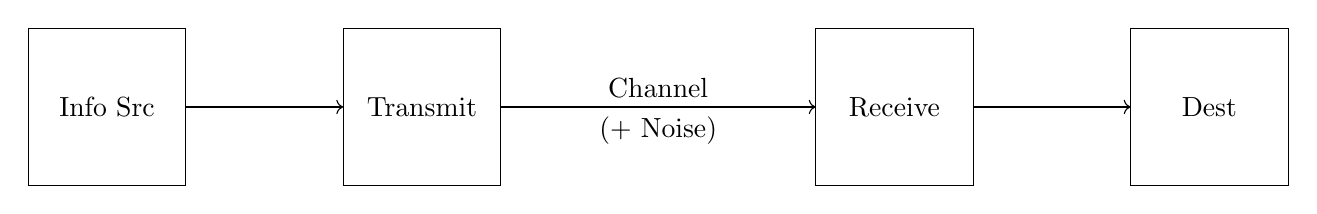
\begin{tikzpicture}[scale=2]
\draw[black] (-4, 0) rectangle (-3, 1) (-2, 0) rectangle (-1, 1) (1, 0) rectangle (2, 1) (3, 0) rectangle (4, 1);
\draw[->] (-3, 0.5) -- (-2, 0.5);
\draw[->] (-1, 0.5) -- (1, 0.5);
\draw[->] (2, 0.5) -- (3, 0.5);
\draw (-3.5, 0.5) node[anchor=center] {Info Src}
    (-1.5, 0.5) node[anchor=center] {Transmit}
    (1.5, 0.5) node[anchor=center] {Receive}
    (3.5, 0.5) node[anchor=center] {Dest}
    (0, 0.5) node[anchor=south] {Channel}
    (0, 0.5) node[anchor=north] {(+ Noise)};
\end{tikzpicture}

\begin{itemize}
\item Infor\textbf{m}ation sources can be m\textbf{o}deled as random variables, probability distributions (LLMs and Chat\textbf{G}PT model language this way).
\item \textbf{Fundamental Counting Principle} (for consec\textbf{u}tive choices): If one event can occur in $n$ ways and a 2nd event can happen in $m$ ways after event one, there are $m \times n$ total possibilitie\textbf{s}.
\item{\textbf{Subsets of a set}: A set of $n$ elements contains $2^n$ subsets.
    \begin{itemize}
        \item For each element of a set, it can either be in the subset or not. 2 possibilities for each of the $n$ elements results in $2^n$ possibilities.
    \end{itemize}
}
\item{\textbf{Permutations}: There are $n!$ permutations of a set of $n$ elements.}
\item{\textbf{Distinguishable Permutations}: Suppose a set of $n$ objects has $k$ distinguishable kinds of objects (e.g. a set of 4 As, 2 Bs, etc.), such that there are $n_1, n_2,\dots n_k$ items in each of the $k$ groups, respectively, with $n_1+n_2+\cdots+n_k=n$ Then the number of ways to arrange the objects is 
\[\frac{n!}{n_1!n_2!\cdots n_k!}\]}

\item \[P(n, r) = \frac{n!}{(n-r)!}\]
\item{\[C(n,k) = \binom{n}{k} = \frac{n!}{k! (n-k)!}\]}
\item Additional reading: Stirling Numbers of the Second Kind
\end{itemize}

\newpage
\subsection{Probability (2024.08.21)}

\paragraph{Sample Space:}
Set of all possible outcomes called $\mathcal{S}$.

\paragraph{Axioms:}
Let $E$ be the event of interest. 

The complement (the event of $E$ \textit{not} happening) is denoted $E^c$

\[0 \le P(E) \le 1\]
\[P(\mathcal{S}) = 1\]

\paragraph{Probability of $E_1$ or $E_2$:}
$P(E_1 \cup E_2) = P(E_1) + P(E_2) - P(E_1 \cap E_2)$

\paragraph{Mutually exclusive:}
$E_1 \cap E_2 = \emptyset$.

Not to be confused with "independent": If events are mutually exclusive, they are completely dependent on each other ($E_1$ happening means $E_2$ did not happen).

If $E_1$ and $E_2$ are independent, then $P(E_1 \cap E_2) = P(E_1) \cdot P(E_2)$

\subsubsection{Exercises}

\paragraph{Exercise 1:}
3 balls are drawn from a bowl of 3 white, 5 black without replacement. What is the probability that 1 ball is white and 2 balls are black?

\[
3 \left[\frac{6\cdot 5 \cdot 4}{11 \cdot 10 \cdot 9}\right] = \frac{C(6, 1) C(5,2)}{C (11, 3)}
\]

\paragraph{Exercise 3:}
5-card hand in poker, P(straight)?

\[\frac{10\left(4^5 - 4\right)}{C(52,5)}\]

\subsection{Discrete Random Variables (2024.08.23)}
\subsubsection{Random Variable:} 
Mapping from sample space $\mathcal{S}$ to real numbers $\mathbb{R}$. Denoted by later capital letters.

\paragraph{Exercise 1:}
Toss 3 fair coins, then Y: \# of heads

\begin{tabular}{ c | c }
$y$ & $P(Y=y)$\\
\hline
0 & ${1}/{8}$ \\ 
1 & ${3}/{8}$ \\ 
2 & ${3}/{8}$ \\ 
3 & ${1}/{8}$ \\ 
\end{tabular}

Describes a discrete \textbf{Probability Mass Function} (vs a continuous \textbf{Probability Density Function, PDF}).

\paragraph{Exercise 2:}
Choose 3 balls randomly selected without replacement from an urn of 20 balls, numbered in order.

\[P(X = i) = \left.{\binom{i-1}{2}} \middle/ {\binom{20}{3}}\right. \]

\subsubsection{Cumulative Distribution Functions (CDFs)}
Let $F$ be a (discrete) cumulative distribution function and $P$ be the probability mass function. $F$ approaches 1 as $a \to \infty$.
\[F(a) = \sum_{x\le a}P(x)\]

\subsubsection{Expected Value}
The expected value of a random variable is given by:
\[
E[X] = \sum_{x\in \mathcal{S}} x P(X = x)
\]

\paragraph{Exercise 4:}
For a fair die,
\[E[X] = \sum_{i=1}^6 i\frac{1}{6}=3.5\]

Notice that $E[X] \not\in \mathcal{S}$.

\paragraph{Exercise 5:}
Let $A$ be an event with probability $P[A]$. Let
\[
I = \begin{cases}
    1 & A \text{ occurs}\\
    0 & A^c \text{ occurs}.
\end{cases}
\]

Then, $E[I] = P[A]$.
\[
\begin{tabular}{c | c}
$x$ & $P(X = x)$ \\
\hline
-1 & 0.2 \\ 
0 & 0.5 \\
1 & 0.3.
\end{tabular}\]

Notice: $E[X^2] = 0.5.$
However, $E[X]^2 = 0.01$

\subsubsection{Functions of Random Variables:} 
If $g(X)$ is a function of the random variable, then
\[E[g(X)] = \sum_{x \in \mathcal{S}} g(x) P(X=x).\]

\textbf{Proof}:
Let $\mathcal{G}$ be the image (i.e. range) of $g(X)$.
Then,

\begin{align*}E[g(X)] &= \sum_{y \in \mathcal{G}} \quad \sum_{x \in \mathcal{S}, g(x)=y}g(x)P(X=x)\\
&=\sum_{y \in \mathcal{G}} y \sum_{x \in \mathcal{S}, g(x)=y}P(X=x)\\
&=\sum_{y\in \mathcal{G}}yP(g(x)=y).\end{align*}

% \begin{align*}E[g(X)] &= \sum_j\sum_{g(x_i)=y_j}g(x_i)P(X=x_i)\\
% &=\sum_jy_j\sum_{g(x_i)=y_j}P(X=x_i)\\
% &=\sum_jy_jP(g(x)=y_j).\end{align*}

Thus, we have the \textbf{Linearity of Expectation}
\[E[aX+b] = aE[X]+b\]

Variance:
\[\text{Var}[X] = E\left[(X-\mu)^2\right],\]

where $\mu = E[X].$ As a result, by expanding and the linearity of expectation,
\[\text{Var}[X]=E[X^2]-E[X]^2.\]

\[\text{Var}[aX+b] = a^2\cdot\text{Var}[X].\]

Also, stdev=$\sqrt{\text{Var}}$


\subsection{Discrete Random Variables 2 (2024.08.27)}

\begin{itemize}
    \item{ \textbf{Bernoulli Random Variable}: $1$ with probability $p$ and $0$ with probability $1-p$. \[E[X] = p \qquad\qquad \text{Var}[X] = E[X^2]-E[X]^2=p-p^2\]}
    \item{\textbf{Binomial Rand Var}: Sum of $n$ independent Bernoulli random variables, each with probability $p$ of being $1$. In other words, $X$ is the number of successes in the $n$ trials.
    \[P(X=k)=\binom{n}{k}p^k(1-p)^{n-k}\]
    \[E[X] = n p \qquad \text{Var}[x] = n p (1-p)\]
    When $p=0.5$, it is symmetrical about the halfway point: $P(X=k) = P(X=n-k)$
    
    \paragraph{Exercise 1:} A player bets on a number from 1-6 and 3 dice are rolled. If the number betted on appears $i$ times for $i\in\{1,2,3\},$ then they win $i$ units, otherwise losing $1$ unit.
\begin{align*}E[X] &= -1\cdot\binom{3}{0}\left(\frac{1}{6}\right)^0\left(\frac{5}{6}\right)^3\\&\quad+1\cdot\binom{3}{1}\left(\frac{1}{6}\right)\left(\frac{5}{6}\right)^2+2\cdot\binom{3}{2}\left(\frac{1}{6}\right)^2\left(\frac{5}{6}\right)+3\cdot\binom{3}{3}\left(\frac{1}{6}\right)^3\left(\frac{5}{6}\right)^0\\&=-\frac{17}{216}<0.\end{align*} So it is unfair.

    \paragraph{Exercise 2:}
    An airplane engine fails in flight with a probability of $1-p.$ If at least $50\%$ of engines work, then the airplane is successful. For what values of $p$ is a 4-engine plane better than a 2-engine plane?
    \begin{align*}
        &P[X_4 < 2] = \binom{4}{0}(1-p)^4+\binom{4}{1}p(1-p)^3\\
        &P[X_2 < 1] = \binom{2}{0}(1-p)^2.
    \end{align*}
    Then,
    \begin{align*}
        P[X_4<2]-P[X_2<1]&=(1-p)^2((1-p)^2+4p(1-p)-1)\\
        &=(1-p)^2(p^2-2p+1-4p^2+4p-1)\\
        &=(1-p)^2(-3p^2+2p)\\
        &=p(p-1)^2(-3p+2).
    \end{align*}
    So, $P[X_4\text{ fails}]>P[X_2\text{ fails}]$ when $p<\frac{2}{3},$ in which case the 2-engine plane is better. Otherwise, when $p>\frac{2}{3},$ a 4-engine plane is better.
    \paragraph{Exercise 3:}
    Let $X$ be a binomial random variable. Then, what are $E[X]$ and $\text{Var}[X]?$

    \begin{align*}
        E[X] &= \sum_{k = 1}^nE[X_k]\\
        &=\sum_{k=1}^np\\
        &=np,
    \end{align*}
    where $X_k$ is Bernoulli. Also, for independent events $E[XY] = E[X]E[Y]$, so:
    \begin{align*}\mathrm{Var}[X+Y] &= E[(X+Y)^2] - E[X+Y]^2 \\&= E[X^2] + E[Y^2] + 2 E[X Y] - E[X]^2 - E[Y]^2 - 2 E[X] E[Y] \\&=\mathrm{Var}[X]+\mathrm{Var}[Y]+2(E[XY]-E[X]E[Y])\\&=\mathrm{Var}[X]+\mathrm{Var}[Y],\end{align*}
    so
    \begin{align*}
        \mathrm{Var}[X] &= \sum_{k=1}^n\mathrm{Var}[X_k]\\
        &=\sum_{k=1}^np(1-p)\\  
        &=np(1-p).
    \end{align*}
    }
\end{itemize}

\subsection{More Random Vars (2024.08.29)}

\subsubsection{Poisson Random Variables}
\[
P(X=k) = e^{-\lambda} \frac{\lambda^k}{k!} \qquad k\in\mathbb{Z}_{\ge 0},\lambda\in\mathbb{R}
\]

Models the probability an event happens $X$ times if it has a probability $p$ of happening every time interval, over the time period of $n$ intervals in the continuous limit as $n\to\infty$ and $\lambda = np$ is a sensible rate. That is, the continuous process where the event has some infinitesimally small probability of happening every instant, yielding a reasonable overall rate of the event happening.

\paragraph{Examples} \url{https://en.wikipedia.org/wiki/Poisson_point_process}. The number of misprints in a page of a book, the number of people entering a queue in a fixed period of time. This distribution can be constructed from binomial distributions:
\begin{align*}
&X: \text{ Binomial rand var } (n, p)\\
&\lambda = n p \qquad (n\to\infty, p\to 0)
\end{align*}
We have
\begin{align*}
P(X=k)&=\frac{n!}{(n-k)!k!}p^k(1-p)^{n-k}
\\&=\frac{n!}{(n-k)!k!}\left(\frac{\lambda}{n}\right)^k\left(1-\frac{\lambda}{n}\right)^{n-k}\\
&=\frac{n(n-1)\cdots(n-k+1)}{n^k}\frac{\lambda^k}{k!}\frac{\left(1-\frac{\lambda}{n}\right)^n}{\left(1-\frac{\lambda}{n}\right)^k}.
\end{align*}
Applying the facts that:
\[\lim_{n\to\infty}\left(1-\frac{\lambda}{n}\right)^n= e^{-\lambda},\]
\[\lim_{n\to\infty}\left(1-\frac{\lambda}{n}\right)^k=1,\]
\[\lim_{n\to\infty}\frac{n(n-1)\cdots(n-k+1)}{n^k}=1,\]
we have
\[P(X=k)\to e^{-\lambda}\frac{\lambda^k}{k!}.\]

Let an item be defective with probability $0.1.$ Then, sample 10 items and calculate
$P(\text{at most 1 defective item}).$
Binomial:
\[\binom{10}{0}(1-p)^{10}+\binom{10}{1}p(1-p)^9\approx0.7361.\]
Poisson:
$\lambda = 10\cdot 0.1=1,$
\[\frac{e^{-1}\cdot 1^0}{0!}+\frac{e^{-1}\cdot 1^1}{1!}\approx 0.7358.\]

\begin{align*}E[X] &= \sum_{k=0}^\infty \lambda e^{-\lambda}\frac{\lambda^k}{k!}\\
&=\lambda e^{-\lambda}\sum_{k=0}^\infty\frac{\lambda^k}{k!}\\
&=\lambda e^{-\lambda}e^{\lambda}\\
&=\lambda.\end{align*}

Also,
\[\text{Var}[X] = E[X^2]-E[X]^2=\lambda.\]
(do the math yourself)

Poisson variables can model the probability of an event happening $k$ times at a constant rate of $\lambda$ in a continuous interval of time/space. In this case, sometimes a Poisson R.V. is written as
\[e^{-\lambda t}\frac{(\lambda t)^k}{k!},\] where $t$ is the time/space interval.


Exercise:
Let an earthquake happen at an average rate of
\[\lambda = \frac{2}{\text{week}}.\]
Then,
\begin{align*}P(\text{at least 3 earthquakes in 2 weeks}) &= 1-(P(0)+P(1)+P(2)).
\end{align*}

We have:
\[P(0)=e^{-\lambda t}=e^{-4},\]
\[P(1)=e^{-\lambda t}\frac{\lambda t}{1!}=4e^{-4},\]
and
\[P(2)=e^{-\lambda t}\frac{(\lambda t)^2}{2!}=8e^{-4}.\]

\subsubsection{Geometric Random Variables}
Given $p$ probability of success, $X$ is the number of trials until the first success.

Then,
\[P(X=k)=(1-p)^{k-1}p,k\in\mathbb{Z}_{>0}.\]
And,
\begin{align*}E[X] &= \sum_{k=1}^\infty k(1-p)^{k-1} p\\
&=\frac{p}{1-p}\sum_{k=1}^\infty k(1-p)^k\\
&=\frac{p}{1-p}\frac{1-p}{p^2}\\
&=\frac{1}{p}.\end{align*}


\subsection{Continuous Random Variables (2024.09.03)}
\subsubsection{Summary of Discrete R.V.}
Know Expected Value and Variance:
\begin{itemize}
    \item Bernoulli (1 with probability $p$, 0 otherwise)
    \[X=\begin{cases}
        0&(1-p)\\
        1&p,
    \end{cases}\]
    \[E[X] = p \qquad \text{Var}[X] = (1-p)p\]
    \item Binomial (sum of $n$ Bernoulli)
    \[X = \sum_n X_{\text{Bernoulli}(p)}\]
    \[P(X = k) = \binom{n}{k} p^k (1-p)^{n-k}\]
    \[E[X] = n p \qquad \text{Var}[X] = n(1-p)p\]
    \item Poisson (\# of occurrences with infinitesimal probability of happening every instant)
    \[X = \lim_{n \to \infty} X_{\text{Binomial}(n,p=\frac{\lambda}{n})}\]
    \[P(X=k) = \frac{e^{-\lambda}(\lambda)^k}{k!}=\frac{e^{-\lambda t}(\lambda t)^k}{k!}\]
    \[E[X] = \lambda \qquad \text{Var}[X] = \lambda\]
    \item Geometric
    \[P(X=k)=(1-p)^{k-1}p\]
    \[E[X] = \frac{1}{p} \qquad \text{Var}[X] = \frac{1-p}{p^2}\]
\end{itemize}


Extra ones for fun:
\begin{itemize}
    \item Negative Binomial Random Variables

    How many trials necessary to get $k$ successes?
    \[P(X=n)=\binom{n-1}{k-1}p^k(1-p)^{n-k},\qquad k\in\{r,r+1,\dots\}.\]
    Geometric R.V. is case where $k=1.$
    \item Hypergeometric Random Variable:
    $m$ white balls, $N-m$ black. Number of white balls out of $n$ chosen.
    \[P(X=k) = \frac{\binom{m}{k}\binom{N-m}{n-k}}{\binom{N}{n}},\qquad k\in\{0,1,\dots,n\}.\]
    As $N\to\infty,$ approaches Binomial/Poisson
    \item look at Zeta distribution
\end{itemize}

\subsubsection{Continuous Random Variables}
\[P(a\le X\le b) = \int_a^b f(x)\,\mathrm{d}x,\]
where $\text{PDF}(x)$ is called the probability density function (pdf).
Also,
\[\int_\mathcal{S}f(x)\mathrm{d}x=\text{usually}\int_{-\infty}^\infty f(x)\diffn(x)=1.\] is this a lebesgue integral lol



Importantly, the height of a pdf isn't a real probability since there are infinite values (and thus a single value has a probability of zero in some sense),
so $P(X=k)$ is nonsensical (or the probability is 0, but the event can still occur). What you can measure is the probability that $X$ is in a specific region.


\paragraph{Exercise 1}
\[f(x) = \begin{cases}
    C(4x-2x^2)&0<x<2\\
    0&\text{otherwise}.
\end{cases}\]
The total probability is
\[1=\int_0^2C(4x-2x^2)\mathrm{d}x=C\left(2x^2-\frac{2}{3}x^3\right)\bigg\vert_0^2=C\left(8-\frac{16}{3}\right),\]
so
\[C=\frac{3}{8}.\]
Then,
\[P(X>1)=\int_1^2f(x)\mathrm{d}x=\frac{3}{8}\int_1^2f(x)\mathrm{d}x=\frac{1}{2}.\]
\paragraph{Exercise 2} The amount of time in hours that a computer functions before it breaks down is given by \[f(x) = \begin{cases}
    \lambda e^{-x/100} & x \ge 0 \\
    0 & x < 0
\end{cases}\]
\[
\int_\mathcal{S} f(x)\,\mathrm{d}x = 1
\]
\[
\therefore \lambda = 1/100
\]
\[
P(50<X<150) = \int_{50}^{150} f(x)\,\mathrm{d}x=e^{-1/2}-e^{-3/2}.\\
\]
\paragraph{Exercise 3}
Lifetime in hours of a certain light bulb is a random variable with pdf
\[
f(x) = \begin{cases}
    0 & x \le 100 \\
    \frac{100}{x^2} & x > 100
\end{cases}
\]
\[P(\text{Exactly 2 of 5 replaced in 150 hours})  = \binom{5}{2}p^2(1-p)^3,\]
where
\[p=\int_{100}^{150}f(x)\diffn{x}=\frac{1}{3}.\]
So,
\[P(\text{Exactly 2 of 5 replaced in 150 hours})=\frac{80}{243}.\]

\paragraph{Cumulative Distributions:}
Cumulative distribution function $F(x)$ is the probability that the random variable is less than $x$:
\[F(x) = \int_{-\infty}^x f(t)\,\mathrm{d}t.\]
Going the other way,
\[\fdiffn{}{a} F(a)=f(a).\]
\paragraph{Exercise 4}
Let $X$ have pdf $f_X(x),$
and $Y=2X.$
Letting
\[F_Y(a)=P(Y\le a)\]
and
\[F_X(a)=P(X\le a),\]
we have
\[P(2X\le a)=P(X\le a/2)=F_X(a/2),\]
so, by chain rule,
\[f_Y(a)=f_X(a/2)\cdot\frac{1}{2}.\]


\paragraph{Expected value}
\[\int_{\mathcal{S}}xf(x)\diffn{x},\]
\[E[g(X)]=\int_{\mathcal{S}}g(x)f(x)\diffn{x}.\]
\paragraph{Variance}
\[E[X^2]-E[X]^2=\int_{\mathcal{S}} x^2f(x)\diffn{x}-\left(\int_{\mathcal{S}} xf(x)\diffn{x}\right)^2.\]
\paragraph{Exercise 5}
Given \textbf{uniform random variable}
\[f(x)=\begin{cases}
    1&0\le x\le 1\\
    0&\text{otherwise},
\end{cases}\]
then
\[E\left[e^X\right]=\int_0^1e^x\diffn{x}=e-1.\]

Now, let $Y=e^X.$ Find $f_Y.$
We have
\[F_Y(a)=P(Y\le a)=P(e^X\le a)=P(X\le \log(a))=F_x(\log(a)).\]
By chain rule,
\[f_y(a)=\frac{f_x(\log(a))}{a}=\begin{cases}
    \frac{1}{a}&1\le a\le e\\
    0&\text{otherwise}
\end{cases}.\]
\subsubsection{Continuous Distributions}

\paragraph{Uniform Random Variables}
\[f(x)=\begin{cases}
    1&0< x<1\\
    0&\text{otherwise}
\end{cases}\]
or
\[f(x)=\begin{cases}
    \frac{1}{\beta-\alpha}&\alpha<x<\beta\\
    0&\text{otherwise}
\end{cases}.\]

\[
E[X] = \frac{\beta + \alpha}{2} \qquad \mathrm{Var}[X] = \frac{1}{12} (\beta - \alpha)^2
\]


\newpage
\subsection{More Continuous Random Variables (2024.09.05)}

\subsubsection{Gaussian Distribution \& Central Limit Theorem}
\[
f(x) = \frac{1}{\sqrt{2\pi} \sigma} e^{-(x-\mu)^2/(2\sigma^2)}\qquad x\in\mathbb{R}.
\]
\[
E[X] = \mu \qquad \text{Var}[X] = \sigma^2
\]

Ignore this:
\[
\mathcal{N}(\mu_1,\,\sigma_1^2) \ast \mathcal{N}(\mu_2,\,\sigma_2^2) = \mathcal{N}\left(\mu_1 + \mu_2,\,\sigma_1^2 + \sigma_2^2\right)
\]

According Laplace, binomial distributions approach a Gaussian distribution as $n\to\infty$. $X$ being a random variable from a normal/gaussian distribution is written as $X \sim \mathcal{N}(\mu,\sigma^2)$.

Do the Gaussian integral by squaring and using polar:
\[
\int_{-\infty}^\infty e^{-x^2}\,\diffn{x} = \sqrt{\pi},
\]
it follows that 
$f(x)$ is normalized with u-sub.
By integrating, letting $X\sim N(0,1),$ then
\[E[X] = 0, \mathrm{Var}[X] = 1.\]
Then, let 
\[Y=aX+b,\]
\[E[Y]=\mu,\]
and
\[\mathrm{Var}[Y] = \sigma^2.\]


\paragraph{Exercise 1}
Let us transmit a binary message (0 or 1) from point A to point B. If I want to send a 1, I send a signal of height 2, and if I want to send a 0, I send a signal of height -2. However, this signal might become disturbed by noise. So, you will receive
\[R=x+N.\]
If $R\ge 0.5,$ we assume that 1 was sent, otherwise we assume a 0 was sent.
Let $N$ be distributed with $N(0,1).$
If I send a 1, then
\[R_1\sim N(2,1),\]
so
\[P[\text{fail}_1]=P[R_1< 0.5]\approx 0.0067.\]
If I send a 0,
then
\[R_2\sim N(-2,1)\]
\[P[\text{fail}_2]=P[R_2\ge -0.5]\approx 0.0730.\]
Then,
\[P[\text{fail}=\frac{1}{2}(P[\text{fail}_1]+P[\text{fail}_2])\approx 0.0365.\]

\subsubsection{Exponential Distribution}
\[
f(x) = \begin{cases}
    \lambda e^{-\lambda x} & x \ge 0 \\
    0 & x < 0
\end{cases}
\]
\[
E[X] = \lambda^{-1} \qquad \text{Var}[X] = \lambda^{-2}
\]

Models the amount of time that passes before an event happens. The relationship between Exponential and Poisson is the same as the relationship between Geometric and Binomial.

More precisely, the probability that the event happens at least once after time $t$ in a Poisson process with rate $\lambda$ is 1 - probability it never happens:
\[
1 - \sum_{k=0}^0 e^{-\lambda t} \frac{(\lambda t)^k}{k!} = 1 - e^{-\lambda t}
\]
Which equals exactly the CDF of the corresponding exponential distribution! The CDF evaluated at $t$ has the interpretation of "the probability the event happened at least once between t=0 and now", which matches up with our calculation from the Poisson distribution.
\[
\int_0^t \lambda e^{-\lambda x} \diffn{x} = 1 - e^{-\lambda t}
\]

\section{Information}
\subsection{Intro to Information (2024.09.11)}

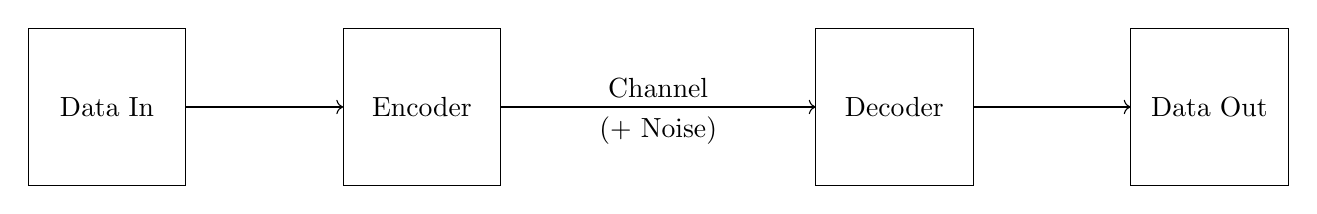
\begin{tikzpicture}[scale=2]
\draw[black] (-4, 0) rectangle (-3, 1) (-2, 0) rectangle (-1, 1) (1, 0) rectangle (2, 1) (3, 0) rectangle (4, 1);
\draw[->] (-3, 0.5) -- (-2, 0.5);
\draw[->] (-1, 0.5) -- (1, 0.5);
\draw[->] (2, 0.5) -- (3, 0.5);
\draw (-3.5, 0.5) node[anchor=center] {Data In}
    (-1.5, 0.5) node[anchor=center] {Encoder}
    (1.5, 0.5) node[anchor=center] {Decoder}
    (3.5, 0.5) node[anchor=center] {Data Out}
    (0, 0.5) node[anchor=south] {Channel}
    (0, 0.5) node[anchor=north] {(+ Noise)};
\end{tikzpicture}

Mathematical formalism: ``Data In'' is the information source (random variable), and the data is a sequence of $k$ symbols where each symbol is the outcome of a random variable.
\[S:\{s_1,s_2,\dots,s_k\}.\]
Encoder acts on blocks of symbols (vectors) and does $\vec{x}=g(\vec{s})$. The encoder's output is a sequence of codewords, which is modeled as another random variable with $m$ different values
\[X:\{x_1,x_2,\dots,x_m\}\]
In transit, noise may be added to the codewords, and this noise is another random variable. The decoder undoes what the encoder did and may also try to correct for noise and errors.

\newpage
\subsubsection{Shannon's Axioms}
\begin{itemize}
    \item Continuity: The amount of information associated with an outcome increases/decreases smoothly (is continuous) as the probability of the outcome changes.
    \item Symmetry: The amount of information associated with a sequence of outcomes does not depend on the order in which the outcomes occur.
    \item Maximal Value: The amount of information associated with a set of outcomes cannot be increased if those outcomes are already equally probably. 
    \item Additive: The information associated with a set of outcomes is obtained by adding the information of individual outcomes. $\text{Info}(\text{1 and 2 and 3}) = \text{Info}(1) + \text{Info}(2) + \text{Info}(3)$
\end{itemize}

Information measures amount of surprise, e.g. if a coin that lands on heads 90\% of the time ends up landing on tails, then you are surprised. So we guess that the surprise amount is $1/p.$ But, if $p=1$ then surprise is 1 (which should be zero) and this isn't additive, so we take the $\log_2:$
\[\log_2\left(\frac{1}{p}\right).\] Assume that all $\log$s are base 2 from here on.

\[
h(x) = -\log(p(x))
\]
Units are bits (this is not a regular cs bit that you nerds know). One bit is the amount of information required to choose between 2 equally likely outcomes. A binary digit (computer science bit), on the other hand, is the value of a binary variable, which is zero or one.

We are interested in the expected/average amount of surprise from an event:
\[X:\{x_1,x_2,\dots,x_,\}\qquad P(X):\{P(x_1),P(x_2)\dots,P(x_m)\}\] 
\begin{align*}
H(X)&=\sum_{i=1}^mP(x_i)\log\left(\frac{1}{P(x_i)}\right)\\
&=E\left[\log\left(\frac{1}{P(X)}\right)\right].
\end{align*}

$H(x)$ is the \textbf{entropy} of the random variable.

\subsubsection{Properties of Entropy}
\begin{itemize}
    \item $H(X)\ge 0.$
    \item $H_b(X)=\log_ba\cdot H_a(X).$
    \item Doubling the number of outcomes increases $H(X)$ by one bit. (Equivalent to flipping a coin + doing the original thing, counting heads + outcome and tails + outcome as different outcomes).
\end{itemize}

\subsection{Entropy Properties (9.13.2024)}
\[H(X)=\sum P(X)\log\left(\frac{1}{P(X)}\right).\]
\paragraph{Example 1}
Fair die with 8 sides.
\[H(X)=\sum_{i=1}^8\frac{1}{8}\log(8)=3.\]

\paragraph{Example 2}
Let
\[X=\begin{cases}
a&p=\frac{1}{2}\\
b&p=\frac{1}{4}\\
c&p=\frac{1}{8}\\
d&p=\frac{1}{8}.
\end{cases}\]
\begin{align*}H(X)&=\frac{1}{2}\log(2)+\frac{1}{4}\log(4)+\frac{1}{8}\log(8)+\frac{1}{8}\log(8)\\&=\frac{1}{2}+\frac{1}{2}+\frac{3}{8}+\frac{3}{8}=\frac{7}{4}.\end{align*}

\paragraph{Example 3}
\[
X = \begin{cases}
    1 & p \\ 0 & 1 - p
\end{cases}
\]
\[
H(p):=H(X) = -p \log(p) - (1-p)\log(1-p)
\]

$H(p)$ is maximized when $p=\frac{1}{2}$ with $H\left(\frac{1}{2}\right)=1$. At the endpoints $H(0) = 0$ and $H(1) = 0$ because you get no information from certain outcomes.

\subsubsection{Jensen's inequality}
$f(x)$ is convex over the interval $(a, b)$ if for every $x_1, x_2 \in (a,b)$ and any $0\le\lambda\le 1,$ then
\[f(\lambda x_1+(1-\lambda)x_2)\le \lambda f(x_1)+(1-\lambda)f(x_2).\]

If $f(x)$ is convex, then $-f(x)$ is concave and obeys the opposite inequality.

Jensen's inequality states that if $f(x)$ is convex over the sample space of $X$ and $X$ is a random variable, then
\[E[f(X)]\ge f(E[X]).\]
\url{https://en.wikipedia.org/wiki/H%C3%B6lder%27s_inequality}

\paragraph{``Proof''} Why is this true?
If $g(x)$ is convex then for some $x_1<c<x_2,$ then for all $x \in [x_1, x_2]$ we have
\[g(x)\ge g(c)+g'(c)(x-c).\] Letting $c=E[X],$
 we have
 \[g(X)\ge g(E[X])+g'(E[X])(X-E[X]).\]
 Taking the expectation of both sides,
 \[E[g(X)] \ge E[g(E[X])]+g'(E[X])E[X-E[X]]=g(E[X]).\]
 \url{https://journalofinequalitiesandapplications.springeropen.com/counter/pdf/10.1186/s13660-016-0985-4.pdf}
\paragraph{Exercise 1}
We know that
\[E[X^2]=\mathrm{Var}[X]+E[X]^2 \implies E[X^2] \ge E[X]^2.\] This is just Jensen's!!!!!

\paragraph{Exercise 2}
$f(x)=-\log(x)$ is convex:
\[E[-\log X]\ge -\log(E[X]).\]
\[\log E[X]\ge E[\log X].\]

\subsubsection{Theorem}
Let $X$ be an R.V. with values $\{x_1,x_2,\dots,x_r\}.$
Prove that \[0\le H(X)\le \log r,\] and $H(X)=0$ if all the $p_i\in\{0,1\}.$
Since each $p_i\le 1,$ we have
\[p_i\log\left(\frac{1}{p_i}\right)\ge 0\implies H(X)\ge 0,\]
and \[p_i\log\left(\frac{1}{p_i}\right) \Longleftrightarrow p_i=0\text{ or }p_i=1,\] so $H(X)=0$ iff each $p_i\in\{0,1\}.$

We have, letting $Y=\frac{1}{p_i}$ with probability $p_i,$
\[H(X)=\sum_i p_i\log\frac{1}{p_i}\le \log\sum_i p_i\frac{1}{p_i}=\log r,\] applying Jensen's with $-\log$ and $Y.$ When $p_i=\frac{1}{r},$ equality occurs, for example.

\paragraph{Exercise $\pi$}
Let \[A=\sum_{n=2}^\infty\left(n\log^2n\right)^{-1},\]
and let $X$ be a Random Variable such that
\[P(X=n)=\frac{1}{An\log^2 n}\] for $n=2,3,\dots$
Prove that $H(X)=\infty.$
\begin{align*}
H(X)&=\frac{1}{A}\sum_{i=2}^\infty\frac{1}{n\log^2n}\log(An\log^2n)\\
&\ge\frac{1}{A}\sum_{i=2}^\infty\frac{\log n}{n\log^2 n}\\
&=\frac{1}{A}\sum_{n=2}^\infty\frac{1}{n\log n}=\infty.
\end{align*}


\paragraph{Exercise 3}
Given $(p_1,p_2,\dots,p_n)$ and some $m$ with $0\le m\le n,$
define
\[q_m=1-\sum_{j=1}^mp_j.\]
Prove that
\[H(p_1,p_2,\dots,p_n)\le H(p_1,p_2,\dots,p_m,q_m)+q_m\log(n-m).\]

\[H(p_, \le H(q)+ q \log(r)\]


\newpage
\subsection{Differential Entropy (2024.09.17)}
 \paragraph{Agastya's 13b solution:}
From 13a, we know that this is just barely possible: At maximum the scale gives us $\log_2(3)$ bits of entropy (from reading left heavy, right heavy, or equal), and the problem to be solved has $\log_2(2\cdot12+1)$ bits of entropy. The counterfeit could be any of the 12 coins, either heavier of lighter, or there might not be a counterfeit. $3\log_2(3) = 4.75$ while $\log_2(2\cdot12+1) = 4.64$! We only have about 0.1 bits of entropy to spare (27 possibilities vs. 25)!

Strategy: Find the number of coins to weigh by considering what will give you the maximum entropy. The probabilities that the scale reads equal, left side heavy, and right side heavy should all be as close to 1/3 as possible. We must also then use the information about which side was heavier from all weighings. 


\begin{itemize}
\item Weigh 4v4. In the case they are equal, these 8 are known good. Then,
\begin{itemize}
   \item Weigh 3 known good vs. 3 unknown. If equal, counterfeit must be the one left out (if there is a counterfeit). Weigh that one left out coin with a known good coin to see if it is counterfeit.


    \begin{itemize}
    \item If the unknown coins are heavier or lighter, we know one is counterfeit and that the counterfeit is heavier or lighter correspondingly. Weigh 1 of the 3 unknowns against another of the 3 unknowns. If equal, the 3rd unknown is counterfeit, and if unequal, counterfeit is the one agreeing with the previous weighing.
    \end{itemize}
\end{itemize}
\item If the 4v4 was unequal, a counterfeit exists. Let's denote the 4 heavier coins as HHHH and 4 lighter as LLLL and 4 known good coins as CCCC. Weigh LLHHH vs. HCCCC
\begin{itemize}
    \item if $LLHHH > HCCCC$, one of the 3 Hs on the left-hand-side is a heavy counterfeit. Weigh 2 of them in a 1v1 and see which is heavier (if equal, the one left out must be heavier).
    \item if $LLHHH = HCCCC$, counterfeit is light and is one of the 2 Ls we left out. Do a 1v1 to see which is the lighter counterfeit.
    \item If $LLHHH < HCCCC$, counterfeit is either one of the 2 Ls on the left-hand-side or the H on the right-hand-side. Weigh the 2 Ls in a 1v1 to see if one is the lighter counterfeit. If they are equal, the heavy one must be the counterfeit.
    \end{itemize}
\end{itemize}


\subsubsection{Differential Entropy}
We have
\[H(X)=\sum p(X)\log\frac{1}{p(X)}.\]
Just like in a Riemann sum, we will split a continuous distribution into many ``bins'' of width $\Delta x.$
$$P(\text{random value X is in a given bin})=\text{proportion of all values in that bin}.$$
Define
\[X^{\Delta}\]
to be the discretized version of $X,$ which is a continuous R.V.
We have
\[H\left(X^{\Delta}\right)=\sum_{i}P(X\in\text{bin}_i)\log\frac{1}{P(X\in\text{bin}_i)}.\]
The probability of $X$ being in the ith bin is the ratio between $a_i,$ which is the the area of the ith bin, to the total area $A:$
\[a_i=n_i\Delta x,\qquad A=\sum a_i,\qquad P_i=\frac{a_i}{A},\qquad \sum P_i=1.\]
We have
\[P_i=P(x_i)\Delta x.\]
\begin{align*}
H\left(X^{\Delta}\right)&=\sum P_i\log\frac{1}{P_i}\\&=\sum P(x_i)\Delta x\log\frac{1}{P(x_i)\Delta x}\\&=\sum P(x_i)\Delta x\log\frac{1}{P(x_i)}+\sum P(x_i)\Delta x\log\frac{1}{\Delta x}.
\end{align*}
Taking the limit, we get
\[\int P(x)\log\frac{1}{P(x)}\diffn{x}+\log\frac{1}{\Delta x}\int P(x)\diffn{x}.\]
Unfortunately, this goes to negative infinity...
So, Differential Entropy is necessary, which would yield
\[h(X)=\int f(x)\log\frac{1}{f(x)}\diffn{x},\]
where $f(x)$ is the pdf of $X.$
(we just ignore the second term lol)


Properties:
\begin{itemize}
    \item If $Y=X+c,$ then $h_y=h_x.$
    \item If $Y=cX,$ then $h_y=h_x+\log c.$
\end{itemize}


\paragraph{Example 1}
Let $X\sim U(0,a).$
Then
\[h(X)=\int_0^a\frac{1}{a}\log a=\log a.\]

If you double the sample size, then $h$ increases by 1, just like discrete entropy. 

Since $h$ can be negative, we treat it with respect to $U(0,1)$ as $h(X \sim U(0,1)) = 0.$ We treat $h$ to mean having more or less information than $U(0,1).$

Differential entropy of an exponential distribution:
\[
h(X) = -\int_0^{\infty} {\lambda e^{-\lambda x} \log(\lambda e^{-\lambda x})\diffn{x}}=\log\left(\frac{e}{\lambda}\right)
\]







Claim:
\begin{itemize}
\item Given a fixed lower and upper bound, a no pdf has a larger entropy than a uniform
\item Given a positive R.V. X with a mean $\mu,$ then the distribution with maximum entropy is an exponential random variable.
\end{itemize}



\subsection{More Entropy (9.19.2024)}
\subsubsection{Aarush Integrates Simplices}
\paragraph{Probability Tuples:}
First, we must define the object we are working with.
\paragraph{Definition}
    We define a \emph{probability tuple} of size $n$ and total probability $a$ as a real tuple $\boldsymbol{p}_{n,a}=(p_1,\ldots,p_n)$ where $0\leq a\leq 1$, and $0\leq p_i\leq 1$ for integers $1\leq i\leq n$, and $\sum_{i=1}^n p_i=a$. 

We need some method to count probability tuples.

\paragraph{Definition}
    We denote the number (measure) of valid probability tuples $\boldsymbol{p}_{n,a}$ as the number $S(n,a)$.

Note that $S(1,a)=1$, since the only tuple is $(a)$. Similarly, $S(2,a)=a$, since $p_1$ can be any value from $0$ through $a$ and $p_1$ uniquely fixes $p_2$. Moreover, for $n\geq 2$, note that there is a bijection between $\boldsymbol{p}_{n,a}$, and the space of probability tuples $\boldsymbol{p}_{n,b}$ as $b$ varies from $0$ to $a$. More specifically,
\begin{equation*}
    S(n,a)=\int_{0}^a S(n-1,a-x)\;dx=\int_{0}^a S(n-1,x)\;dx.
\end{equation*}
Using this equation we get that
\begin{equation*}
    S({n,a})=\frac{a^{n-1}}{(n-1)!}.
\end{equation*}

We define a random variable $X_n=(x_1,\ldots,x_n)$ to be a random probability tuple $\boldsymbol{p}_{n,1}$, where $X_n$ is equally likely to be every distinct probability tuple. Our goal is to find the probability distribution for $P(x_1=k)$ for some $0\leq k\leq 1$.

To do this, we will find the cumulative probability distribution by finding the probability $P(x_1\leq k)$. Say a tuple $\boldsymbol{p}_{n,a}$ has $p_1\geq k$. Then, we can subtract $k$ from $p_1$ to get a probability tuple $\boldsymbol{p}'_{n,a-k}$. In other words, there is a bijection between these two objects. Thus, to count the tuples $\boldsymbol{p}_{n,a}$ where $p_1\leq k$, we can use complementary counting, which then gets the cumulative distribution of
\begin{equation*}
    P(x_1\leq k)=\frac{S(n,1)-S(n,1-k)}{S(n,1)}=1-(1-k)^{n-1},
\end{equation*}
The $S(n,1-k)$ counts the number of probability tuples where we can add $k$ to one of the probabilities $p_1<1-k$ so that the tuple sums to 1, so $S(n,1-k)$ counts the number of n-tuples summing to 1 where $p_1 > k$. Alternatively, we can integrate over all possibilities for $p_1 < k$ and write this as
\begin{equation*}
    P(x_1\le k) = \frac{1}{S(n,1)}\int_0^k S(n-1,1-p)\diffn{p} = 1-(1-k)^{n-1}.
\end{equation*}
Thus, we can calculate the probability distribution function as
\begin{equation*}
    P(x_1=k)=\frac{d}{dk}P(x_1\leq k)=(n-1)(1-k)^{n-2}.
\end{equation*}
\paragraph{Expected Information:}
Let $H(x)=-x\log_2(x)$, and $H(x_1,\ldots,x_n)=\sum_{i=1}^n H(x_i)$. Then, the expected amount of information from a probability distribution is
\begin{align*}
    E(H(X_n))&=E\left(\sum_{i=1}^n H(x_i)\right)=\sum_{i=1}^n E(H(x_i))=n\cdot E(H(x_1))\\
    &=n\cdot\int_0^1 P(x_1=k)\cdot H(k)\;dk\\
    &=-n(n-1)\cdot \int_0^1 (1-k)^{n-2}\cdot k\cdot \log_2(k)\diffn{x},
\end{align*}
which we simplify using Mathematica to get
\begin{equation*}
    E(H(X_n))=\frac{H_n-1}{\ln(2)},
\end{equation*}
where $H_n=\sum_{i=1}^n\frac{1}{i}$.

\subsubsection{Funny Discrete Problem}
Go back to discrete:
Given $(p_1,p_2,\dots,p_n)$ and some $m$ with $0\le m\le n,$
define
\[q_m=1-\sum_{i=1}^mp_i = \sum_{i=m+1}^n p_i.\]
Prove that
\[H(p_1,p_2,\dots,p_n)\le H(p_1,p_2,\dots,p_m,q_m)+q_m\log(n-m).\]
\[H(p_{m+1},\dots,p_n) \le H(q_m)+ q_m \log(n-m)\]
Let
\[z=H(p_{m+1},\dots,p_n)=\sum_{i=m+1}^n p_i \log\parens{\frac{1}{p_i}}\]
% \le q_m \log\parens{\frac{1}{q_m}} + q_m \log(n-m)
Divide by $q_m:$
\[\frac{z}{q_m}=\sum_{i=m+1}^n \frac{p_i}{q_m} \log\parens{\frac{1}{p_i}}\]
Add $\log q_m:$
\[\frac{z}{q_m}+\log q_m=\sum_{i=m+1}^n\frac{p_{i}}{q_m}\log\frac{q_m}{p_{i}},\]
let this be $H(Y).$
Then,
\[z=H(p_{m+1},\dots,p_n)=q_m(H(Y)-\log q_m).\]

But, we have $H(Y)\le \log(n-m)$ from maximal entropy,
so
\[q_m(H(Y)-\log q_m)\le q_m\log\frac{1}{q_m}+q_m\log(n-m),\]
and thus
\[H(p_1,p_2,\dots,p_n)\le H(p_1,p_2,\dots,p_m,q_m)+q_m\log(n-m).\]


\subsubsection{Differential Entropy of Gaussian R.V.}
\[f(x)=\frac{1}{\sqrt{2\pi\sigma^2}}e^{-x^2/{2\sigma^2}}.\]
\begin{align*}
h(X)&=-\frac{1}{\ln 2}\int_{-\infty}^\infty f(x)\ln f(x)\diffn{x}\\
&=-\frac{1}{\ln 2}\int_{-\infty}^\infty f(x)\left(-\frac{x^2}{2\sigma^2}-\ln\sqrt{2\pi\sigma^2}\right)
\\&=-\frac{1}{\ln 2} \left( \frac{-E[X^2]}{2\sigma^2}-\ln\sqrt{2\pi\sigma^2} \right)\\
&=-\frac{1}{\ln 2} \left( \frac{-E[X^2]}{2\sigma^2}-\frac{1}{2}\ln2\pi\sigma^2 \right).
\end{align*}
But, $E[X^2]=\sigma^2+\mu^2=\sigma^2,$
so
\[h(X)=\frac{1}{2 \ln 2}\parens{1+\ln 2\pi\sigma^2}=\frac{1}{2}\log_2(2\pi e\sigma^2).\]

\subsubsection{Source Coding}


Source $\to$ message $\to$ Encoder $\to$ signal

We want a code for English text because america, specifically, we want a scheme to map letters to a sequence of $0$'s and $1$'s.

\begin{tabular}{c c}
    A&00000\\
    B&00001\\
    C&00010\\
    $\vdots$&$\ddots$
\end{tabular}


This uses 5 bits, but it is bad.
\paragraph{Exercise 1}
Let $E=0,$ $T=1,$ $A=01,$ but A=ET????!?!???!?
bad
\paragraph{Exercise 3}
Now try
$E=1,$ $T=011,$ $A=1110,$ $O=10011,$ $I=01110,$

But now
011101110011 is both IAT and TEIT, so decoding is not unique.
\paragraph{Exercise 3}
Let $E=0,$ $T=10,$ $A=110,$ $O=111.$

Now, 00100110111010 is uniquely EETEAOET.

The difference between the second and third encodings is that no code in the third encoding has a prefix equal to another code.

\subsection{Lagrange \& Source Coding (9.23.2024)}
\subsubsection{Review}
We want a uniquely decodable code better than 5 bits per letter that is also instantaneous (like a DFA), otherwise known as prefix-free. 



We call a code non-singular if every element in X maps to a different string. So
\[x_i\ne x_r\implies C(x_i)\ne C(x_j).\]

We call a code uniquely decodable if any decoded string has only one possible source string that produced it.

We call a code a prefix code or an instantaneous code if no codeword is the prefix of any other codeword. 

Instantaneous codes are a subset of uniquely decodable codes, which are a subset of non singular codes, which are a subset of all codes.
Example:


\begin{tabular}{|c|c|c|c|c|}
\hline
 X&Singular&\makecell{Nonsingular but \\ not uniquely decodable}&\makecell{Uniquely Decodable \\ but not Instantaneous}&Instantaneous\\ 
 \hline
 1 & 0 & 0   & 10 & 0 \\
 2 & 0 & 010 & 00 & 10 \\
 3 & 0 & 01  & 11 &  110 \\
 4 & 0 & 10 & 110 &111 \\
 \hline
\end{tabular}
\paragraph{Exercise 1}
\[X=\begin{tabular}{|c|c|c|}
\hline
Number&Probability&Code\\
\hline
    1 &  1/2 & 0\\
    2 &  1/4 & 10\\
    3 & 1/8 & 111 \\
    4 & 1/8 & 111\\
    \hline
\end{tabular}\]

We see that $H(X)=1.75\,\si{bits}$ and $E[\text{length}] = \mathcal{L}(C)=1.75.$
\paragraph{Exercise 2}
\[X=\begin{tabular}{|c|c|c|}
\hline
Number&Probability&Code\\
\hline
    1 &  1/3 & 0\\
    2 &  1/3 & 10\\
    3 & 1/3 & 11 \\
    \hline
\end{tabular}\]

We see that $H(X)=\log(3)\,\si{bits}$ and $\mathcal{L}(C)=\frac{5}{3}\,\si{bits}.$ Note that \[H(X)\approx 1.585<\mathcal{L}(C)\approx 1.667.\] 

\subsubsection{Huffman Code}
This is a way to encode any source with an probability distribution into bits. In short, the more probable a word is, the fewer bits its codeword has.
Algorithm:
\begin{itemize}
    \item Find the two least probable symbols (\textit{e.g.}, letters)
    \item Combine the two letters to make an imaginary composite symbol. This composite has a probability of the sum of the probabilities of each event.
    \item Repeat this process until you have one symbol left.
    \item For every time you combine two symbols, assign the top path with a 1 and the bottom path with a zero
    \item Make it a tree by concatenating binary numbers the lead to that symbol.
\end{itemize}

\paragraph{Exercise 3}

\begin{tabular}{|c | c | c | c| c|}
    \hline
    A & \multicolumn{3}{c|}{0.87 (1)} & \multirow{5}{*}{1.00 (root)} \\
    \cline{2-4}
    B & 0.04 (1) & \multirow{2}{*}{0.08 (1)} & \multirow{4}{*}{0.13 (0)} & \\
    \cline{2-2}
    C & 0.04 (0) & & & \\
    \cline{2-3}
    D & 0.03 (1) & \multirow{2}{*}{0.05 (0)} & & \\
    \cline{2-2}
    E & 0.02 (0) & & & \\
    \hline
\end{tabular}

\medskip
The two least probable symbols are D and E, so make DE with probability 0.05. Then we combine B and C with the lowest probabilities of 0.04 and 0.04 to make BC with probability 0.08. Continue this, and make a tree


\subsubsection{Lagrange Multipliers and (Constrained) Optimization}


The problem: Maximize scalar function $f(\vec{v})$ under the constraints $c_i(\vec{v}) = 0$.

Solution: Solve for $\nabla f(\vec{v}) = \sum_i \lambda_i \nabla c_i(\vec{v})$. The values of the $\lambda_i$ do not matter, only the value of $\vec{v}$.

If the gradient of $f$ does not lie purely in the space spanned by the gradients of the constraints, then we can always increase $f$ by moving along the constraint manifold (moving along the constraint manifold = moving in a direction perpendicular to the gradients of the constraint functions, think about contours of constant value). Adding constraints removes constraints on the gradient of $f$.


\paragraph{Exercise 4}
Maximize $f(x,y)=3x+4y$ with $g(x,y)=x^2+y^2-1=0.$
We turn this constrained problem into an unconstrained maximum of a new function $\phi(x,y,\lambda).$
Definition: \[\phi(x,y,\lambda)=f(x,y)-\lambda g(x,y).\]

The gradient is
\[\nabla\phi(x,y,\lambda)=\begin{bmatrix}
\frac{\partial f}{\partial x}+\lambda \frac{\partial g}{\partial x}\\
\frac{\partial f}{\partial y}+\lambda \frac{\partial g}{\partial y}\\
g(x,y)
\end{bmatrix}=\vec{0}.\]
So,
\[\begin{bmatrix}
    3+2\lambda x\\
    4+2\lambda y\\
    x^2+y^2-1
\end{bmatrix}=\vec{0}.\]
So, $4\lambda^2=25,$ and thus $\lambda=\pm \frac{5}{2}.$ Then,
\[x=\frac{3}{5},y=\frac{4}{5}.\]

\paragraph{Exercise 5}
Optimize $f(x,y,z)=xyz$ given $x^2+y^2+z^2=12.$
We have
\[\begin{bmatrix}
    yz+2\lambda x\\
    xz+2\lambda y\\
    xy+2\lambda z\\
    x^2+y^2+z^2-12
\end{bmatrix}=\vec{0}.\]

So, \[x=y=z=2.\] 


\subsection{Lagrange 2 (9.30.2024)}
Maximize discrete entropy:
\[   H(p_1,p_2,\dots,p_n) = -\sum_i p_i \log p_i \]

Under the constraint function:
\[C(p_1,p_2,\dots,p_i)=-1 + \sum_i p_i = 0\]

Lagrange multipliers:
\begin{align*}
    \Phi(p_1,p_2,\dots,p_i,\lambda) &= \nabla H - \lambda\nabla C \\
    &= \begin{bmatrix}
        -\log p_1-1\\
        -\log p_2-1\\
        \dots\\
        -\log p_n-1
    \end{bmatrix} -\lambda\begin{bmatrix}
        1\\1\\\dots\\1
    \end{bmatrix} = 0
\end{align*}
Using additional knowledge that $0\le p_i \le 1$, we know that $p_i=\frac{1}{n},$ for $1\le i\le n,$ and thus $H=\log n.$



\paragraph{Continuous} Given a continuous distribution that is bounded with
\[a\le x\le b,\]
prove that the uniform distribution maximizes entropy. \medskip 

We want to maximize 
\[\int f(x)\log\frac{1}{f(x)}\diffn{x},\] given
\[\int f(x)\diffn{x}=1.\]

Let 
\[\phi(f)=\int f(x)\log\frac{1}{f(x)}\diffn{x}-\lambda\left(\int f(x)\diffn{x}-1\right).\]


\begin{figure}[!ht]
\centering
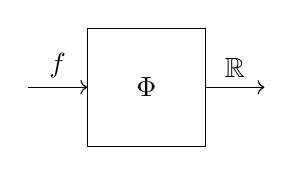
\begin{tikzpicture}[scale=0.75]
    \draw (-1,-1) rectangle (1, 1) (0,0) node {$\Phi$};
    \draw[->] (-2,0) -- (-1,0);
    \draw[->] (1,0) -- (2,0);
    \draw (-1.5, 0) node[anchor=south] {$f$} (1.5,0) node[anchor=south] {$\mathbb{R}$};
\end{tikzpicture}
\end{figure}

We want to perturb $f$ slightly and see how $H(f)$ changes.

Perturb the range $f(x)$ to $f(x+\delta)$ by $\epsilon.$ How much does $\phi$ change?
\[\Phi(f_{perturbed})-\Phi(f)=\left((f(x)+\epsilon)\log\frac{1}{f(x)+\epsilon}-f(x)\log\frac{1}{f(x)}\right)\delta-\lambda\left((f(x)+\epsilon)\delta-1-(f(x)\delta-1)\right).\]

After algebra and factoring out a delta,
\[(f(x)+\epsilon)\log\frac{1}{f(x)+\epsilon}-f(x)\log\frac{1}{f(x)}-\lambda(f(x)+\epsilon-f(x)).\]

So,
\[\epsilon\left(\frac{d}{dz}z\log\frac{1}{z}\right)\bigg\vert_{z=f(x)}-\lambda\epsilon=0.\]

So, 
\[f(x)=e^{-1-\lambda}\] is constant, so $f$ is uniform.

\paragraph{Problem}
Find $p_0,p_1,p_2,\dots$ so that
\[\sum_i p_i\log\frac{1}{p_i}+\log\Delta x\]
is maximized,
given
\[\sum_ip_i\Delta x=1\]
and
the mean is contrained:
\[\sum_i ip_i\Delta x^2=\mu\]
is constant.

We have
\[\Phi(p_1,p_2,\dots,\Delta x,\lambda_1,\lambda_2)=\sum_{i}p_i\log\frac{1}{p_i}+\log\Delta x-\lambda_1\left(\sum_ip_i\Delta x -1\right)-\lambda_2\left(\sum_i ip_i\Delta x^2-\mu\right).\]

Taking the gradient,
\[\nabla\Phi=\begin{bmatrix}
    -\log p_0-1-\lambda_1\Delta x^2\\
    -\log p_1-1-\lambda_1\Delta x-\lambda_2\Delta x^2\\
    -\log p_2-1-\lambda_1\Delta x-2\lambda_2\Delta x^2\\
    \dots\\
    -\log p_i-1-\lambda_1\Delta x-i\lambda_2\Delta x^2\\
    \dots\\
    \sum_i p_i\Delta x-1\\
    \sum_i ip_i\Delta x^2-\mu
\end{bmatrix}\]

You can solve this, and get
\[p_i=\frac{1}{\mu}e^{-x/\mu}.\]

\section{Source Coding}
\subsection{Source Coding Theorem (10.2.2024)}

Goal: Construct instantaneous codes of minimum expected length. 
We know that you cannot assign short codewords to all source symbols if we want the code to still be instantaneous.

\subsubsection{Kraft Inequality}
\[\sum_{i=1}^m \mathcal{D}^{-\ell_i}\le 1,\]
Where $\mathcal{D}$ is the alphabet size (\textit{e.g.}, binary codes have $\mathcal{D}=2$), and the codeword lengths are $\ell_1,\ell_2,\dots,\ell_m.$ Conversely, given a $\mathcal{D}$ and $\ell_i$ that satisfy this inequality, there exists an instantaneous code with lengths $\ell_i.$

Proof:
Let $\mathcal{D}=2$ because that's all we care about honestly.
Consider a binary tree, with each node having 2 children and each branch is a symbol of some codeword. Each leaf is a codeword (for now).


No prefixes means that no codeword is the descendant of another codeword . Let $\ell_{max}$ be the length of the longest set of codewords. Now, grow out the tree to length $\ell_{max}$ for all branches.
A codeword at level $\ell_i$ has
\[2^{\ell_{max}-\ell_i}\] leaf descendants. The leaf descendants of each codeword form $m$ disjoint sets because no codeword is the descendent of another. The total number of nodes in these leaf descendants must be at most $2^{\ell_{max}},$ so for we have $\sum_{i=1}^m 2^{\ell_{max}-\ell_i} \le 2^{\ell_{max}}$ (remember disjoint sets). Thus:
\[\sum_{i=1}^m2^{-\ell_i}\le 1.\] This same idea works for all $\mathcal{D}.$

\subsubsection{Minimum Codeword Length}
Minimize expected binary codeword length $L=\sum_i p_i\ell_i$ for $\ell_1,\ell_2,\dots,\ell_m$ satisfying 
\[\sum_i 2^{-\ell_i}\le 1.\]

Pretend it's an equality trust me bro.

\[\Phi=\sum_i p_i\ell_i-\lambda\left(\sum_i 2^{-\ell_i}-1\right),\]
\[\implies \frac{\partial\Phi}{\partial\ell_i}=p_i+\lambda 2^{-\ell_i}\ln2=0.\]
\[2^{-\ell_i}=\frac{-p_i}{\lambda\ln 2}.\] Substitute this into the contsraint that
\[\sum_{i=1}^m 2^{-\ell_i}=1,\]
\[\sum_{i=1}^m\frac{-p_i}{\lambda\ln 2}=-\frac{1}{\lambda\ln 2}=1,\]
\[\lambda=\log_2(e)\] and the optimal length
\[\ell_i^\ast=-\log_2 p_i.\]
This means that the average length
\[\mathcal{L}^\ast=\sum_i p_i\ell_i^\ast=H(X)!!!!\] Small problem, $\ell_i$ should be integral but it's fine...


\subsubsection{Source Coding Theorem:}
The expected length $\mathfrak{L}$ of a binary codeword is greater than or equal to the entropy:
\[\mathfrak{L}\ge H(X),\]
with equality iff $2^{\ell_i}=p_i.$

Proof:
\[\mathfrak{L}-H(X)=\sum_ip_i(\ell_i+\log p_i)=\sum_ip_i(-\log_22^{-\ell_i}+\log_2 p_i)=\sum_i p_i\log\frac{p_i}{r_i}-\log c,\]
where
\[r_i=\frac{2^{-\ell_i}}{\sum_i 2^{-\ell_i}}\]
and
\[c=\sum_i 2^{-\ell_i}.\]
Consider now 
\[-\sum p_i\log\frac{p_i}{r_i}=\sum p_i\log\frac{r_i}{p_i}\le\log\sum p_i\frac{r_i}{p_i}=\log\sum r_i=\log 1=0,\] by Jensen. This means that $\mathfrak{L}\ge H(X).$

\subsection{Huffman is Optimal (2024.10.07)}
(? rohan please help) Proof that a huffman code achieves optimal avg codeword length within 1 bit of lower bound:

\[\ell_i = \left\lceil \log_2 \frac{1}{p_i} \right\rceil \]
Lengths of codewords satisfy Kraft's inequality (instantaneous code):
\[\sum 2^{-\ell_i} = \sum 2^{-\left\lceil \log \frac{1}{p_i} \right\rceil} \le \sum2^{-\log \frac{1}{p_i}} = \sum p_i = 1 \]
We have
\[ \log \frac{1}{p_i} \le \ell_i \le \log \frac{1}{p_i} + 1 \]
Taking expected value of everything:
\[H(X) \le L \le H(X) + 1 \quad \blacksquare \]

\paragraph{Lemma:} For any probability distribution (without loss of generality, assume that $p_1 \ge p_2 \ge \dots \ge p_m$), there exists an optimal instantaneous code (of minimum expected codeword length) such that 
\begin{itemize}
    \item[1.] If $p_j > p_k$, then $\ell_j \le \ell_k$.
    \begin{itemize}
        \item We consider swapping codewords. Say we have code $C_m'$ which is $C_m$ but with the codewords for $j$ and $k$ swapped.
        \begin{align*}
        L(C_m') - L(C_m) &= \sum p_i \ell_i' - \sum p_i l_i \\
        &= p_j \ell_k + p_k \ell_j - p_j \ell_j - p_k \ell_k \\
        &= (p_j - p_k) (\ell_k - \ell_j)
        \end{align*}
        Because $C_m$ is an optimal code, the left-hand side $L(C_m') - L(C_m) \ge 0$. By definition, $p_j - p_k > 0$, therefore $\ell_k - \ell_j \ge 0. \quad \blacksquare$
    \end{itemize}
    
    %\item[2.] The two longest codewords have the same length and differ only in the last bit.
    %\begin{itemize}
    %    \item Proof by Contradiction: assume that the 2 longest codewords have differing lengths. Then, we can delete the last bit of the longest and still be instantaneous (definition of instantaneous codes) so that code cannot have been optimal. By property 1, the longest codewords are the least likely symbols.

    %    ok aarush i did not understand what you did, please help
    %    \[\sum 2^{-\ell_i} = 1 \qquad 2^{\ell_m} \sum 2^{-\ell_i}\]
    % end{itemize}
      \item[2.] The two longest codewords have the same length and differ only in the last bit.
    \begin{itemize}
        \item Proof by Contradiction: assume that the 2 longest codewords have differing lengths. Then, we can delete the last bit of the longest and still be instantaneous (definition of instantaneous codes) so that code cannot have been optimal. By property 1, the longest codewords are the least likely symbols.

        \item Alternatively (thanks Aarush), Kraft's inequality will hold with equality if a code is optimal. Therefore,
        \[\sum 2^{-\ell_i} = 1 \implies \sum 2^{\ell_{max}-\ell_i} = 2^{\ell_{max}}\]
        The right-hand side is necessarily even, but if there is only one code with the longest length, the left-hand side will be odd, as that term will be 1 and the rest will be powers of 2.
    \item[3.] And these longest codewords correspond to the two least likely symbols.
    \end{itemize}
    \begin{itemize}
        \item Not all optimal codes have this property, but by rearranging the $0$ and $1$ labels on the tree, I can find a code that does satisfy this.
    \end{itemize}
\end{itemize}

% \begin{itemize}
%     \item Property 2) If there is a max length codeword without a sibling, we can delete the last bit, reducing average length and contradicting optimality.
%     \item Thus, every max length codeword in \emph{any} optimal instantaneous code has a sibling.
% \end{itemize}


Actual proof stuff: We want to prove that if a code satisfies those properties, it can be thought of as a Huffman code.

Create a ``merged" code $C_{m-1}$ with $m-1$ symbols from $C_m$ as follows: Take the common prefix of the two longest codewords and allot it to a (fictional) symbol with probability $p_{m-1} + p_m$, keeping all other codewords the same. Define $p_i$ and $\ell_i$ for $C_m$ and $p_i'$ and $\ell_i'$ for $C_{m-1}$: for $0\le i < m-1$, $p_i' = p_i$ and $\ell_i' = \ell_i$. For the two merged symbols, $p_{m-1}' = p_{m-1} + p_{m}$ and $\ell_{m-1}' = \ell_m - 1 = \ell_{m-1} - 1$. Thus, removing the 2 longest codewords from an optimal instantaneous code:
\begin{align*}
    L(C_m) &= \sum p_i \ell_i \\
    &= \sum_{i=1}^{m-2} p_i' \ell_i' + (p_{m-1} + p_m) (\ell_{m-1}' + 1) \\
    &= \sum_{i=1}^{m-1} p'_i \ell_i' + (p_{m-1} + p_m) \\
    &= L(C_{m-1}) + p_{m-1} + p_m,
\end{align*}

Minimizing $L(C_m)$ is the same as minimizing $L(C_{m-1})$ This process of combining the 2 lowest probability symbols is why Huffman works: Repeat the process down to 1 symbol, and you have created a Huffman tree which is optimal as $L(C_1) = 0$.

\section{Guest Speaker: Dr. Subramanian}
\subsection{Large Language Model: an Information Theory Approach}
In 1952, Shannon wrote a paper on the information of the English language, talking about average entropy and average word length. He figured this out by counting words in a library.
\begin{itemize}
\item Bag of words distribution (0th order model):
Cut out words of a text, place them in a bag, and pick them out randomly. Really stupid but a good start. Surprisingly good, for example sentiment analysis just counts ``happy'' and ``sad'' words. 

Zipf's ``law:'' bag of words plot sorted in decreasing order; looks like $\frac{1}{n},$ this law has been observed in many different languages.

\item Unigram model (1st order model):
Words depend on the previous word, so we let the probability distribution depend on the previous word, so each word corresponds to the probability distribution of the next word, forming a table. From this, you can generate text, and this is pretty garbage but not as bad as the 0th order method.
\item Bigram moddel (2nd order model):
Each pair of two words correspond to a probability distribution of the third word. This is better than first model but still pretty garbage.

The English dictionary has about a million words, of which 100k are used often enough. In the second order case, there are a $100000^2$ entries in the table. 


\item ChatGPT is just an n-gram model for $n=32776.$ Practically, it's just a table with 32777 columns and 100k rows. Obviously $100000^{32776}$ is too ridiculously large to store. But in reality, the pdfs are pretty sparse, so most words have almost zero probability. This means that this table is compressible. In order to compress this, companies like Google managed to compress this to about 1 billion parameters (which is really good compared to the original size). In short, they made a neural network that takes in 32776 words as an input and outputs a probability distribution: \url{https://arxiv.org/abs/1706.03762}. Then everyone makes a bunch of LLM's, like Gemini, Llama, GPT, Grok ai, Claude, etc. But, they all are really the same concept fundamentally, regardless of what the hype is. 
\end{itemize}



Occam's Razor: If there are multiple explanations, believe the simplest one, all things equal. For example, Kepler's simple laws validated the pages and pages of measurements that had been made of the positions of the planets, so obviously you should follow Kepler's laws. Then, Newton's law of gravity explains the planets, so you should prefer Newton's laws.

In the AI world, we think of underfitting and overfitting. For example, if we have five equations and three variables, we don't have enough degrees of freedom (underfitting), while if we have five equations and seventeen variables, we have too many degrees of freedom (overfitting). In AI, this is the comparison between the amount of training data and the amount of parameters. Occam's razor would say to find the best fit that's not too simple (i.e., don't overfit and don't underfit). In an LLM, you need to find the right number of parameters to not overfit or underfit. What industry is doing is increasing the number of parameters until the model starts overfitting to figure out the optimal LLM. 

Four powerhouses of AI: MIT by Minsky, Stanford by McCarthy, CMU by Simon, IBM by Solomonoff. In the 1980's, when Reagan became president, people said that you shouldn't give funding to ``random'' people unless for military. Someone that got funding snipped was Geoffrey Hinton, who was working on the unpopular subject of Neural Networks. The first neural network was a perceptron, and people knew that two layers are enough given a large enough hidden layer:
\url{https://en.wikipedia.org/wiki/Universal_approximation_theorem}, but people didn't yet figure out how to train networks with backpropagation, so people thought hidden layers were pointless. However, Minsky showed that XOR isn't possible without a hidden layer, so people thought Neural Networks were useless. So, Hinton moved to Canada because they are nicer people. He then worked on his own without any recognition or care that people said it was stupid to work on NN's. He came up with many innovations in Neural Networks. He went to the ImageNet competition, and in 2012 he got 96\% accuracy which was insane. 
\subsubsection{Vision Foundation Models}
People are trying to apply LLM techniques to images (vision foundation models), just how humans can think in both words and images. Instead of looking at each word, think of ``filling in the blanks'' of the image by removing some small parts of the image and asking the NN to fill it in. How do you train? Well, ChatGPT sampled the entire internet and gave it complete training data to figure out the 32777th word. In reality, supervised and reinforcement learning are the only realistic training strategies. Supervised learning is ``monkey see, monkey do,'' while reinforcement learning is ``doggy do good thing, doggy gets biscuit.'' Unsupervised learning didn't seem like real learning until the ``fill in the blank'' concept happened: self-supervised learning. The internet creates its own ``fill in the blank'' puzzles for the Neural Network to solve. Google London is working on this a lot. 


\subsubsection{``Attention is all you need''} keep spamming the attention block throughout the paper. Attention block: sharpen a probability distribution by increasing the high probability values and attenuating the low probability values. You can also do blunting, which is the opposite. These are calculated based on the Temperature parameter, $T=0$ is sharpening to the extreme case, $T=\infty$ is blunting to uniform case. We want somewhere in the middle. This is based on the Boltzmann definition of the temperature. ``softargmax'' formula:
\[q_i=\frac{e^{p_i/T}}{\sum_ie^{p_i/T}}:=\frac{e^{p_i/T}}{Z}.\]
if $0\le T\le 1$ it sharpens, if $1\le T\le\infty$ it blunts it.

\[
\mathrm{Attention}(Q,K,V) = \mathrm{softmax}\left(\frac{Q K^T}{\sqrt{d_k}}\right) V
\]


\subsubsection{Hallucinations}
Why did it take so long from 2017 to make AI a big deal? 

AI is really wasteful for power consumption, every single ChatGPT query uses so much Energy. So people decided that it's way too computationally expensive to publish AI because there aren't enough computers to supply the world. Meanwhile, Sam Altman tried to be like ``500 users limited edition,'' and other companies were pressured to follow suit, the only company who played their cards well was Microsoft funding OpenAI at arm's length, keeping OpenAI responsible in case it doesn't work and making Microsoft profitable if it works. Big challenge of AI: Try to reduce power consumption by $10^6.$ Back to hallucinations: people expect that ChatGPT is some divine power that knows everything, but in reality it's just a monkey pulling words out of a jar. BUT HALLUCINATIONS ARE INTENDED, IT'S PROBABILITY ONLY!!!




\subsubsection{RAG (Retrieval Augmented Generation)}
It's a hack that tries to lower hallucination:
\begin{itemize}
    \item Looks on google for some documents
    \item ``Based on the above documents, what is Boltzmann's role ...''
\end{itemize}
\subsubsection{General Comments}
There is a science in Data Science: Statistics in new garb, instead of $\mu$ and $\sigma,$ Data Science uses billions of parameters. While Statisticians were very cautious about making mistakes.
\begin{itemize}
\item Sampling Bias
\item You have to call it out in advance to say something is lucky, machine learning guys do cross-validation by holding back some of the data, then checking to see if it works
\end{itemize}




\section{More Source Coding}
\subsection{Shannon-Fano-Elias Code (10.11.24)}

% \begin{tikzpicture}
%     \draw (0,0) node {A} (1,1.5) node {B} (2,3) node {C} (3,1.5) node {D} (4,0) node {E} (2,0) node {F};
% \end{tikzpicture}

Instead of using pdf, we use cumulative distribution. If $p(x)>0,$ then define $F(x)=\sum_{a\le x}p(a)$ for all $x.$ Looking at the graph vertically, you can think of it as a partition of the unit interval, since $0\le F(x)\le 1.$
Define
\[\bar{F}(x):=\frac{1}{2}p(x)+\sum_{a< x}p(a).\] $\bar{F}$ is surjective, hence we can turn it into a code. But, $\bar{F}$ is real, which requires infinite bits!!! So, if we use an approximate value of $\bar{F},$ how much accuracy do we need? $\bar{F}$ just gives the point in the middle of the ranges for each codeword, which is the optimal point to ``aim for'' with our binary decimal approximation.

Truncate $\bar{F}$ to $\ell(x)$ bits:
\[\lfloor\bar{F}(x)\rfloor_{\ell(x)}.\] We use the first $\ell(x)$ bits of $\bar{F}(x)$ as a code for $x.$ Clearly,
\[\bar{F}(x)-\lfloor\bar{F}(x)\rfloor_{\ell(x)}<\frac{1}{2^{\ell(x)}}.\]
If $\ell(x)=\lceil\log\frac{1}{p(x)}\rceil+1,$ then
\[\frac{1}{2^x}<p(x)/2=\bar{F}(x)-F(x-1).\] This lets you decode. Thus, $\ell(x)$ bits is enough to describe $x.$ We also want prefix-free codes. Consider a codeword
\[z_1z_2\dots z_\ell\in\{0,1\}^{\ell}\] and an interval corresponding to it of 
\[\left[0.z_1z_2\dots z_{\ell},0.z_1z_2\dots z_{\ell}+\frac{1}{2^{-(\ell+1)}}\right].\]

The lower end of the interval is in the lower half of the step and the upper half is below the top of the step. Thus, this interval lies within the entire step.


\begin{tabular}{c|c|c|c|c|c|c}
    $x$ & $p(x)$ & $F(x)$ & $\bar{F}(x)$ & binary[$\bar{F}(x)$] & $\ell(x)$ & codeword\\
    \hline
     1& 0.25& 0.25& 0.125& 0.001& 3& 001\\
     2& 0.5& 0.75& 0.5& 0.10& 2& 10\\
     3& 0.125& 0.875& 0.8125& 0.1101& 4& 1101\\
     4& 0.125& 1& 0.9375& 0.1111& 4& 1111
\end{tabular}.

This code isn't very good, for example because the last digit is pointless. Average length: 2.75, Entropy=1.75. Huffman code achieves this entropy so it is optimal.

We want to bound the average length of the codeword:
\[L(x)=\sum p(x)\ell(x)=\sum p(x)\left(\left\lceil\log\frac{1}{p(x)}\right\rceil+1\right)<H(X)+2\]


\subsubsection{Arithmetic Coding}
Associate each codeword to a subinterval of $[0,1]$ $[a,b).$ Choose a number in the subinterval and encode the number in binary. Arithmetic codes become better when you have entire words as opposed to separate symbols. Also, if the source pdf changes, we dont have to completely rewrite the code.

\paragraph{Visualizing Arithmetic Codes}
Ruler Intervals: Focus on one inch of a ruler and put a tickmark at the halfway point, splitting it into two intervals $\left[0,\frac{1}{2}\right)$ and $\left[\frac{1}{2},1\right),$ or, in binary $[0,0.1)$ and $[0.1,1)$ in binary. Then split each interval again in half:
\[[0,0.01)\qquad[0.01,0.10)\qquad[0.10,0.11)\qquad[0.11,1),\] making the tick marks smaller than the half tick. Repeat forever, so that $1/2$ has tallest tickmarks, $1/4$ and $3/4$ have the next tallest, etc. 
\paragraph{Examples}
Given $[0.52,0.92),$ the tallest tickmark is at $0.75.$ In general, where is the tallest tickmark for any interval $[a,b).$ If $b-a\ge\frac{1}{2^m},$ then the tallest tickmark has the same height of $\frac{1}{2^m},$ where
\[m\le\log\left\lceil\frac{1}{b-a}\right\rceil.\]
you get the idea

Given an interval $[a,b)\in[0,1),$ what is the fattest interval in it. Given $[0.52,0.92),$ we don't a half or quarter inch interval fully contained in it, we only have intervals of an eighth wide:
\[[0.625,0.75),[0.75,0.875).\]
We take the smallest tallest interval:
\[m=\left\lceil\frac{2}{b-a}\right\rceil=\left\lceil\log\frac{1}{b-a}\right\rceil+1\]
The smallest tallest tickmark corresponds to the slimmest fattest interval that is completely contained in $[a,b).$


\begin{tabular}{c|c}
     $x$&$p(x)$  \\
     \hline
     0&0.2\\1&0.4\\2&0.4 
\end{tabular}
Let's try to encode 210. We split the unit interval into 0.2, 0.4, 0.4, and then split each subintervale into 0.2, 0.4, 0.4 of it, and so on.


\begin{tabular}{c|c|c}
     2 &  &\\
     &  &\\
     \hline
     1& & \\
     & & \\
     \hline
     0 & & 
\end{tabular}


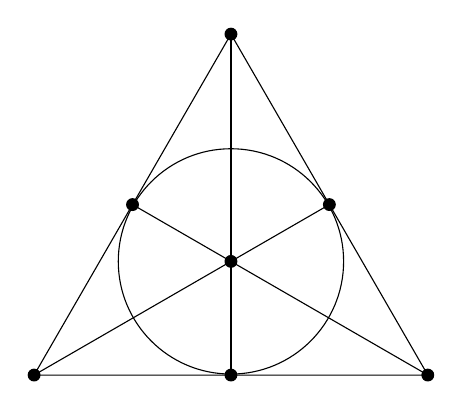
\begin{tikzpicture}[
mydot/.style={
  draw,
  circle,
  fill=black,
  inner sep=1.5pt}
]
\draw
  (0,0) coordinate (A) --
  (5cm,0) coordinate (B) --
  ($ (A)!.5!(B) ! {sin(60)*2} ! 90:(B) $) coordinate (C) -- cycle;
\coordinate (O) at
  (barycentric cs:A=1,B=1,C=1);
\draw (O) circle [radius=5cm*1.717/6];
\draw (C) -- ($ (A)!.5!(B) $) coordinate (LC); 
\draw (A) -- ($ (B)!.5!(C) $) coordinate (LA); 
\draw (B) -- ($ (C)!.5!(A) $) coordinate (LB); 
\foreach \Nodo in {A,B,C,O,LC,LA,LB}
  \node[mydot] at (\Nodo) {};    
\end{tikzpicture}

\subsection{Arithmetic Codes + Conditional Probability (10.15.2024)}
Review Fano Code

\begin{tabular}{c|c|c|c|c|c|c}
$x$&$p(x)$&$F(x)$&$\bar{F}(x)$&$\bar{F}(x)$ in binary&$\ell(x)$&cw\\
\hline
1&0.25&0.25&0.125&$0.0001$&3&000\\
2&0.25&0.5&0.375&$0.011$&3&001\\
3&0.2&0.7&0.6&$0.1\overline{0011}$&4&1001\\
4&0.15&0.85&0.775&$0.110\overline{0011}$&4&1100\\
5&0.15&1&0.925&$0.111\overline{0110}$&4&1110\\
\end{tabular}

$H(X)=1.891.$

Back to Arithmetic Codes:
Let
\[X\in\{0,1,2\}\]
and
\[p=\{p_0,p_1,p_2\}=\{0.2,0.4,0.4\}.\]
We want to send 210. Split up the interval: the interval of 2 is $[0.6,1).$ The interval of 21 is $[0.6+0.4\cdot 0.2,0.6+0.4\cdot 0.6)=[0.68,0.84).$ The interval of 210 is $[0.68,0.68+0.2\cdot0.4\cdot0.4)=[0.68,0.712).$

Now we want to encode this interval:
\[\frac{0.712+0.68}{2}=0.696\approx 0.101100_b,\] truncating to $\lceil\log(1/0.032)+1\rceil$ bits. In other words, we find (the lower bound of) the largest binary interval that is fully contained in $[0.68,0.712).$

\textbf{Example \#2}

Let
\[X\in\{0,1,2, 3\}\]
and
\[p=\{0.05,0.05,0.5, 0.4\}.\]

The message we want to send is 2320, which lies in the interval $[0.42, 0.425)$. The length of our code word will be $\lceil -\log(0.5 \cdot 0.4 \cdot 0.5 \cdot 0.05) \rceil + 1 = 9$. The midpoint of the interval, $0.4225$, encoded in binary and truncated to nine bits is 011011000. \\

\textbf{Optimality}

Let
$X\in\{0,1, ..., m\}$
and
$p=\{p_0,p_1, ..., p_m\}$.
Consider the probability distribution of all words $X_1,X_2,\dots.$
We have
\[\ell(x)\le\left\lceil \log
\frac{1}{p^\ast(x)}\right\rceil+1=\ell_{sh}(x)+1,\]
where $p^{\ast}(x)=p_{x_1}p_{x_2}\dots p_{EOF}$ is the length of the interval.
So the expected length
\[L^{\ast}=\sum \ell(x)p^{\ast}(x)\le L_{sh}+1<H(X)+2.\] So it's pretty good.


\section{Conditional Probability}
\subsection{Conditional Prob (2024.10.17)}
\textbf{Definition}: Given two events E and F, the probability that E occurs given that F occurs is
\[P(E|F)=\frac{P(E\wedge F)}{P(F)}\]
where $P(E\wedge F)$ is the probability that both E and F occur.

e.g. probability that 3 tosses are heads given at least one head:
\[P=\frac{P(\text{3 tosses and at least 1 head})}{P(\text{at least one head})}=\frac{1/8}{7/8}=\frac{1}{7}.\]

\paragraph{Bridge Example}:
North and South vs East and West. We know that North and South have 8 spades between them. What is the probability that East has 3 of the remaining spades.
\[P=\frac{\binom{5}{3}\binom{21}{10}}{\binom{26}{13}}.\]

Extension:
\[P(E_1E_2\dots E_n)=P(E_1)P(E_1|E_2)P(E_3|E_2E_1)\cdots P(E_n|E_1E_2\dots E_{n-1}).\]
Let us have 52 cards that are randomly split into 4 piles of 13 cards each. What is the probability that each pile has exactly one Ace?
\[E_1: \text{ace of spades in one of the piles}\qquad E_2: \text{ace of spaces and hearts are in different piles}\dots.\]
\[P(E_1)=1.\]
\[P(E_2|E_1)=\frac{39}{51}.\]
\[P(E_3|E_1E_2)=\frac{26}{50}.\]
\[P(E_4|E_1E_2E_3)=\frac{13}{49}\]
Go multiply.


\subsubsection{Bayes' Rule}
\begin{align*}P(E)&=P(EF)+P(EF^C) \\
&= P(E|F) P(F) + P(E|F^C) P(F^C).\end{align*}
This is the law of the excluded middle lol.
\[P(A|B)P(B) = P(B|A)P(A) = P(\text{A and B}) = P(\text{B and A})\]

\paragraph{Example} A lab blood test is 95\% effective in detecting disease when actually present, and has a 1\% false positive rate for healthy patients. If 0.5\% of the population actually have the disease, what is the probability that a person has the disease given a positive test?

Remembering $P(T) = P(T|D) P(D) + P(T|D^C) P(D^C)$:
\[P(D|T) = \frac{P(T|D) P(D)}{P(T)} = \frac{0.95 \cdot 0.005}{0.005\cdot0.95 + 0.995 \cdot 0.01} = \boxed{32.3\%}\]

\subsubsection{Independent Events}
If and only if $E$ and $F$ are independent events, then $P(E|F) = P(E)$ and $P(F|E) = P(F)$. Then, $P(\text{E and F}) = P(E) P(F)$.

Do not confuse ``mutually exclusive'' with ``independent!'' They are actually opposites.


\subsubsection{Joint Distributions}
\[p(x,y) = P(X=x\,\&\&\,Y=y)\]
\[F(a,b) = P(X\le a\,\&\&\,Y\le b)\]
This is 2D instead of 1D: we can make a table to represent the joint distribution, and we should double sum/double integrate.
\[p_x(x) = P(X = x) = \sum_y p(x,y)\]
\[p_y(y) = P(Y = y) = \sum_x p(x,y)\]


Consider a set of three red balls, four white balls, and five blueballs
Choose 3 balls at random, and let
$X$ be the number of Red balls and $Y$ the number of white balls.

\begin{tabular}{c|c|c|c|c|c}
    $x\downarrow$ $y\rightarrow$& 0 & 1 & 2 & 3&margin  \\ \hline
     0 & & & &\\ \hline
     1 & $\frac{\binom{3}{1}\binom{5}{2}}{\binom{12}{3}}$&$\frac{\binom{3}{1}\binom{4}{1}\binom{5}{1}}{\binom{12}{3}}$&$\frac{\binom{3}{1}\binom{4}{2}}{\binom{12}{3}}$&0&add them up\\\hline
     2 & & & &\\ \hline
     3 & & & & \\ \hline
\end{tabular}

Looking at $p_x(x)$, we sum the table along the rows $y$ so its the marginal thing.
\[P(x\in A,y\in B)=\int_B\int_Af(x,y)\diffn{x}\diffn{y}.\]

\[F(a,b)=\int_{-\infty}^b\int_{-\infty}^a f(x,y)\diffn{x}\diffn{y}.\]

\[f(a,b)=\frac{\partial^2}{\partial a\partial b}F(a,b).\]
\[f_x=\int f(x,y)\diffn{y},f_y=\int f(x,y)\diffn{x}.\]
\paragraph{Example}
a) 
\[P(X>1,Y>1)=\int_1^\infty\int_1^\infty 2e^{-x}e^{-2y}\diffn{y}\diffn{x}=\frac{1}{e^3}.\]
b)
\[P(X<Y)=\int_0^\infty\int_0^yf(x,y)\diffn{x}\diffn{y}=\frac{1}{3}.\]
c)
\[P(X<a)=\int_a^\infty\int_0^\infty f(x,y)\diffn{y}\diffn{x}=1-e^{-a}.\]

$X:f_x,Y:f_y,$ what is the pdf of $X+Y?$
\[F_{x+y}=P(X+Y\le a)=\int_{-\infty}^\infty\int_{-\infty}^{a-y}f_x(x)f_y(y)\diffn{x}\diffn{y}=\int_{-\infty}^\infty F_x(a-y)f_y(y)\diffn{y}.\]
CONVOLUTION!!!


\subsection{Conditional Expectation and Distributions (10.23.24)}
\paragraph{Exercise}
Choose a point randomly in a circle with radius R such that all regions within the circle are equally likely.
\[f(x,y)=\begin{cases}
    c&x^2+y^2\le R^2\\
    0&\mathrm{otherwise}.
\end{cases}\]
\[c=\frac{1}{\pi R^2}.\]
We have the marginal distributions
\[f_x=\int_{-\infty}^\infty f(x,y)\diffn{y}=2c\sqrt{R^2-x^2}=\frac{2\sqrt{R^2-x^2}}{\pi R^2}.\] Similarly,
\[f_y=\frac{2\sqrt{R^2-y^2}}{\pi R^2}.\]
The probability that the distance from the origin is $\le a$ is
\[\frac{a^2}{R^2}.\]
The expected value of the distance is
\[\int_{-\infty}^\infty\int_{-\infty}^\infty \sqrt{x^2+y^2}f(x,y)\diffn{x}\diffn{y}=\frac{1}{\pi R^2}\int_0^R\int_0^{2\pi} r^2\diffn{\theta}\diffn{r}=\frac{1}{\pi R^2}\frac{2\pi R^3}{3}=\frac{2}{3}R.\]


If you have two independent Random Variables X and Y, we want to find out $f_{x+y},$ which is
\[\frac{\diffn{}}{\diffn{a}}F_{x+y}(a)=\int_{-\infty}^\infty\frac{\partial}{\partial a}F_x(a-y)f_y(y)\diffn{y}=\int_{-\infty}^\infty f_x(a-y)f_y(y)\diffn{y}=f_x\ast f_y.\] This is only for independent variables.

The sum of two poisson random variables is another poisson random variable, where the $\lambda$ rates of the R.V.s just add together. Intuition of Poisson point process.
\subsubsection{Conditional Distributions}
Discrete:
\[p_{X|Y}(x|y)=P(X=x\,|\,Y=y)=\frac{P(X=x,Y=y)}{P(Y=y)}.\] The cumulative mass function is
\[P_{X|Y}(x|y)=P(X\le x\,|\,Y=y)=\sum_{a\le x}p_{X|Y}(a|y).\]

\paragraph{Example}
Let
\[P(X=0,Y=0)=0.4,P(X=0,Y=1)=0.2,P(X=1,Y=0)=0.1,P(X=1,Y=1)=0.3.\]
Given $Y=1,$ then
\[P(X=0|Y=1)=0.4,P(X=1|Y=1)=0.6.\]

\paragraph{Example 2}
Let $X$ and $Y$ be independent poisson R.V. with $\lambda_1$ and $\lambda_2.$
Find the conditional distribution of $X$ given $X+Y=n.$ Since the sum of two independent Poissons is a poisson with $\lambda=\lambda_1+\lambda_2.$

\[P(X=k, Y=n-k) = \frac{(\lambda_1)^k}{k!} e^{-\lambda_1} \frac{(\lambda_2)^{n-k}}{(n-k)!} e^{-\lambda_2}\]

\begin{align*}P(X+Y=n) &= 
\sum_{k=0}^n P(X=k,Y=n-k) \\ &= \sum_{k=0}^n \frac{(\lambda_1)^k (\lambda_2)^{n-k}}{k!(n-k)!} e^{-\lambda_1-\lambda_2} \\&= \sum_{k=0}^n \binom{n}{k}\frac{(\lambda_1)^k (\lambda_2)^{n-k}}{n!}e^{-\lambda_1-\lambda_2} \\ &=
\frac{(\lambda_1+\lambda_2)^n}{n!}e^{-\lambda_1-\lambda_2}
\end{align*}

\begin{align*}P(X=k|X+Y=n)&=\left.\left(\frac{(\lambda_1)^k (\lambda_2)^{n-k}}{k! (n-k)!}e^{-\lambda_1}e^{-\lambda_2}\right)\middle/\left(\frac{(\lambda_1+\lambda_2)^n}{n!}e^{-\lambda_1-\lambda_2}\right) \right. \\ &=
\frac{\binom{n}{k}\lambda_1^k\lambda_2^{n-k}}{(\lambda_1+\lambda_2)^n}\\&=\binom{n}{k}\left(\frac{\lambda_1}{\lambda_1+\lambda_2}\right)^k\left(\frac{\lambda_2}{\lambda_1+\lambda_2}\right)^{n-k}.\end{align*}
You can verify that this sums to one by binomial.

Continuous:
\[f_{X|Y}(x|y)=\frac{f(x,y)}{f_y(y)}.\]
\paragraph{Exercise}
\[f(x,y=\begin{cases}\frac{12}{5}x(2-x-y)&0<x<1,0<y<1\\
0&\mathrm{otherwise}.
\end{cases}\]
We have
\[f_{X|Y}(x|y)=\frac{f(x,y)}{f_y(y)}.\]
\[f_y(y)=\int_{0}^1 f(x,y)\diffn{x}=\frac{8}{5}-\frac{6}{5}y\]

\[f_{X|Y}(x|y)=\frac{ \begin{cases}\frac{12}{5}x(2-x-y)&0<x<1,0<y<1\\
0&\mathrm{otherwise}
\end{cases}}{{\frac{8}{5}-\frac{6}{5}y}}=\frac{6x^2-12x+6xy}{3y-4}\mathds{1}_{(0,1)\times(0,1)}.\]

\subsection{More Conditional Stuff 10.25.2024}
For two random variables X and Y, with join distribution $p(x,y),$ we can easily find 
$E[X]\text{ and }E[Y]$.

We want to find the covariance between $X$ and $Y.$ Recall that with $\mu_x = E[X]$, we have
\[Var[X]=E[(X-\mu_x)^2].\]
We define the covariance of $X$ and $Y$ to be the following, with $\mu_x=E[X],\mu_y=E[Y].$
\begin{align*}
\mathrm{Cov}(X,Y)&=E[(X-\mu_x)(Y-\mu_y)] \\
&= E[XY-\mu_xY-\mu_yX+\mu_x\mu_y]=E[XY]-\mu_x\mu_y.
\end{align*}

\paragraph{Properties of Covariance}
See \url{https://en.wikipedia.org/wiki/Covariance#Relationship_to_inner_products}. The covariance is bilinear and symmetric.
\[\mathrm{Cov}(X,Y)=\mathrm{Cov}(Y,X),\]
\[\mathrm{Cov}(X,X)=\mathrm{Var}[X].\]

Consider $X_1,X_2,\dots,X_n$
and
$Y_1,Y_2,\dots,Y_n.$
Then
\[\mathrm{Cov}\left(\sum_i X_i,\;\sum_j Y_j\right)=\sum_i\sum_j\mathrm{Cov}(X_i,Y_j).\]

Also,
\[\mathrm{Cov}\left(\sum_iX_i,\;\sum_iX_i\right)=\sum_i \mathrm{Var}X_i+2\underset{i<j}{\sum\sum}\mathrm{Cov}(X_i,X_j).\]
\[\mathrm{Var}\left(\sum_iX_i\right)=\sum_i\mathrm{Var}(X_i)\]
if the $X_i$ are independent.

\paragraph{Conditional Expectation:}
\begin{align*}E[X|Y=y]&=\sum_x xP(X=x|Y=y)=\sum_x p_{x|y} \\
&=\int xf_{x|y}\diffn{x}. \qquad \text{(continuous)}\end{align*}

\paragraph{Example 1}
Let X and Y be iid binomial R.V.'s, both with parameters $n$ and $p.$
Find
\[E[X|X+Y=m].\]


\[E[X|X+Y=m]=\sum_{i=0}^n k\frac{\binom{n}{i}\binom{n}{m-i}}{\binom{2n}{m}}=\frac{m}{2}.\]
This is a hypergeometric distribution.
\paragraph{Exercise 2}
\[f(x,y)=\frac{e^{-x/y}e^{-y}}{y}.\]
With $x,y>0.$

\[E[X|Y=y]=\int_0^\infty x\frac{f(x,y)}{\int_0^\infty f(x,y)\diffn{x}}\diffn{x}=y.\]

\subsubsection{Joint \& Conditional Entropy}
\[H(X,Y) = -\sum_x \sum_y p(x,y) \log p(x,y) = -E_{p(x,y)}[\log p(x,y)]. \]
\begin{align*}H(Y|X) &= \sum_x p(x) H(Y|X=x) \\ 
&= -\sum_x p(x) \sum_y p(y|x) \log p(y|x) \\
&= -\sum_x \sum_y p(x,y) \log \frac{p(x,y)}{p(x)}\end{align*}


\paragraph{Chain Rule}
\[H(X,Y)=H(X)+H(Y|X)=H(Y)+H(X|Y).\]

\begin{align*}H(X,Y)&=-\sum_x\sum_y p(x,y)\log p(x,y)\\&=-\sum_x\sum_y p(x,y)(\log p(x)+\log p(y|x))\\&=-\sum_x\sum_y p(x,y)\log p(x)-\sum_x\sum_y p(x,y)\log p(y|x)\\&=H(X)+H(Y|X).\end{align*}
By symmetry, this is also
\[H(Y)+H(X|Y).\]

\paragraph{Relative Entropy}
``Distance'' between two distributions. See \url{https://en.wikipedia.org/wiki/Kullback%E2%80%93Leibler_divergence}: it is the difference between cross-entropy and entropy.

\[D(p||q)=\sum p(x)\log\frac{p(x)}{q(x)}.\]


\subsection{Relative Entropy and Mutual Information (10.30.2024)}

\begin{tabular}{c|c|c|c|c|c}
    $y \downarrow$ $x \rightarrow$ & 1 & 2 & 3 & 4 & $\sum$ \\
    \hline
    1 & $2^{-3}$ & $2^{-4}$ & $2^{-5}$ & $2^{-5}$ & $2^{-2}$\\
    \hline
    2 & $2^{-4}$ & $2^{-3}$ & $2^{-5}$ & $2^{-5}$ & $2^{-2}$ \\
    \hline
    3 & $2^{-4}$ & $2^{-4}$ & $2^{-4}$ & $2^{-4}$ & $2^{-2}$ \\
    \hline
    4 & $2^{-2}$ & $2^{-\infty}$ & $2^{-\infty}$ & $2^{-\infty}$ & $2^{-2}$ \\
    \hline
    $\sum$ & $2^{-1}$ & $2^{-2}$ & $2^{-3}$ & $2^{-3}$ & $2^{0}$ \\
    
\end{tabular}
\medskip

\textbf{a} $H(X) = 7/4$

\textbf{b} $H(Y) = 2$

\textbf{c} $H(X|Y)=1.375$

\textbf{d} $H(Y|X)=1.625$

\textbf{e} $H(X,Y)=H(X|Y)+H(Y)+H(Y|X)+H(X)=3.375$


\paragraph{KL DIVERGENCE IS NOT SYMMETRIC} But, it can measure how close these two distribtutions are, but it measures how inefficient $q$ is w.r.t. $p,$ so if you knew $p,$ then $q$ represents how inefficient a coding of $q$ would be.
\begin{align*} 
D(p||q) &= H_x (p || q) - H(p) \\
&= \sum p(x) \log \frac{1}{q(x)} - \sum p(x) \log \frac{1}{p(x)}
\end{align*}
The first term is the average number of bits created from sampling from the distribution of $p(x)$ if you had thought the distribution were actually $q(x)$ (cross-entropy). Thus, you can think of KL divergence as the number of bits you would waste if you used a Huffman coding for $q(x)$ to encode $p(x)$.

\subsubsection{Mutual Information}
\[I(X;Y)=\sum\sum p(x,y)\log\frac{p(x,u)}{p(x)p(y)}=D(p(x,y)||p(x)p(y)).\]
Note that if $x$ and $y$ are indpendent, then $p(x,y)=p(x)p(y),$ so $I(X;Y)$ would be zero, as expected. $I$ represents how inefficient you are if you assume they are independent but they actually aren't.

Relation between Mutual Information and Entropy:
\begin{align*}
I(X;Y)&=\sum p(x,y)\log\frac{p(x,y)}{p(x)p(y)} \\&=\sum p(x,y)\log\frac{p(x|y)p(y)}{p(x)p(y)}\\&=\sum\log p(x|y)-\sum p(x,y)\log p(x)\\&=-\sum p(x)\log p(x)-\left[-\sum p(x,y)\log p(x|y)\right]\\&=H(X)-H(X|Y)\\&=H(X)+H(Y)-H(X,Y).
\end{align*}

\subsection{More Mutual Information (11.01.2024)}
\begin{align*}
D(p||q)&=\sum p(x)\log\frac{p(x)}{q(x)}.
\\
H(X,Y)&=\sum p(x,y)\log\frac{1}{p(x,y)}.
\\
H(Y|X)&=-\sum p(x)H(Y|X=x)=\sum p(x,y)\log\frac{1}{p(y|x)}.
\\
H(X,Y)&=H(X)+H(Y|X).
\\
I(X;Y)=I(Y;X)&=\sum p(x,y)\log\frac{p(x,y)}{p(x)p(y)}=D(p(x,y)||p(x)p(y))=H(X)-H(X|Y).
\end{align*}

\begin{figure}[h]
\centering
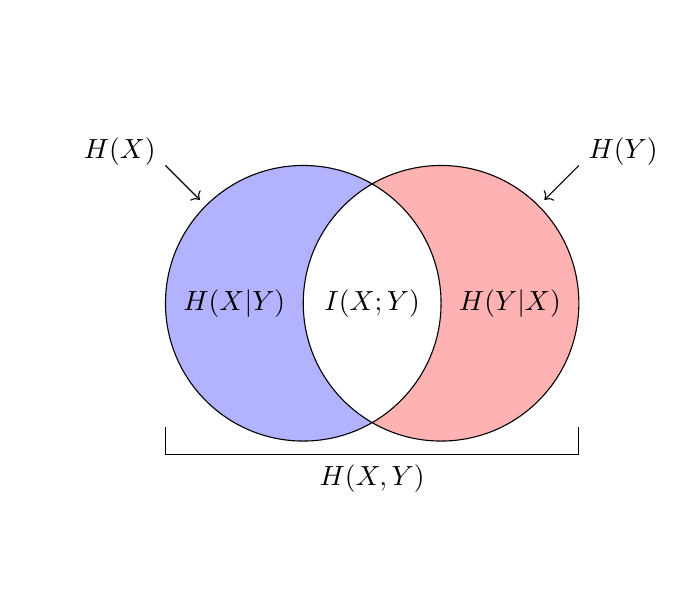
\begin{tikzpicture}[fill=gray,scale=1.75]
% left hand
\scope
\clip (-2,-2) rectangle (2,2)
      (1,0) circle (1);
\fill[blue!30] (0,0) circle (1);
\endscope
% right hand
\scope
\clip (-2,-2) rectangle (2,2)
      (0,0) circle (1);
\fill[red!30] (1,0) circle (1);
\endscope

\draw[->] (-1,1) -- (-0.75, 0.75);
\draw[->] (2,1) -- (1.75, 0.75);
\draw (2,1.1) node[anchor=west] {$H(Y)$} (-1,1.1) node[anchor=east] {$H(X)$};

\draw (-1,-0.9) -- (-1,-1.1) -- (2,-1.1) -- (2,-0.9) (0.5,-1.1) node[anchor=north] {$H(X,Y)$};

% outline
\draw (0,0) circle (1) (-0.5,0)  node [text=black] {$H(X|Y)$}
      (1,0) circle (1) (1.5,0)  node [text=black] {$H(Y|X)$}
      (0.5,0) node[text=black] {$I(X;Y)$} ;
      
      %(-2,-2) rectangle (3,2) node [text=black,above] {$H$};
\end{tikzpicture}
\end{figure}
\begin{enumerate}
\item If $X_1,X_2,\dots,X_n$ are identical, then (Faraday's law of induction):
\[H(X_1,X_2,\dots,X_n)=\sum_{i=1}^n H(X_i\big|[X_{i-1},\dots,X_1]).\]

\item (Square brackets denote grouping for readability.)
\[I([X;Y]\big|Z)=H(X\big|Z)-H(X\big|[Y,Z]).\]
\item
\[D(p(x,y)||q(x,y))=D(p(x)||q(x))+D(p(y|x)||q(y|x)).\]

\end{enumerate}

\paragraph{Theorem:} Kullback-Leibler divergence is positive ($D(p||q)\ge0$)
\[D(p||q)=\sum p(x)\log\frac{1}{q(x)}-H(p(x)).\]
This is the same as proving Gibb's inequality because KL divergence is the difference between cross-entropy and entropy. Lagrange multipliers:
\[\Phi=\sum p_i\log\frac{1}{q_i}-\lambda\sum_i q_i,\]
\[\frac{\partial\Phi}{\partial q_i}=-\frac{p_i}{q_i\ln(2)}-\lambda=0,\]
\[q_i=-\frac{p_i}{\lambda\ln(2)}.\]
\[\sum_{i}q_i=-\sum_i\frac{p_i}{\lambda\ln(2)}=1,\]
so $q_i=p_i,$ where
\[\sum_i p(i)\log\frac{1}{q_i}=H(p)\] is a minimum,
so 
\[D(p||q)\ge 0.\]

\begin{align*}
    -D(p||q) &= \sum p(x) \log \frac{q(x)}{p(x)} \\
    &\le \log \sum p(x) \frac{q(x)}{p(x)} = \log 1 = 0
\end{align*}
This also means that \[I(X;Y)=D(p(x,y)||p(x)p(y))\ge 0,\] and equality occurs iff $X$ and $Y$ are independent. 
\paragraph{Example}
\[H(X)\le\log|\mathscr{X}|,\]
where \[|\mathscr{X}|\] denotes the number of elements in $X$ with equality iff $X$ is uniform.
If 
\[u(x)=\frac{1}{|X|},\] and $p(x)$ is the mass function of $X,$ then
\[D(p||u)=\log|\mathscr{X}|-H(X)\ge 0,\] so QED.

\subsubsection{Channel Capacity}
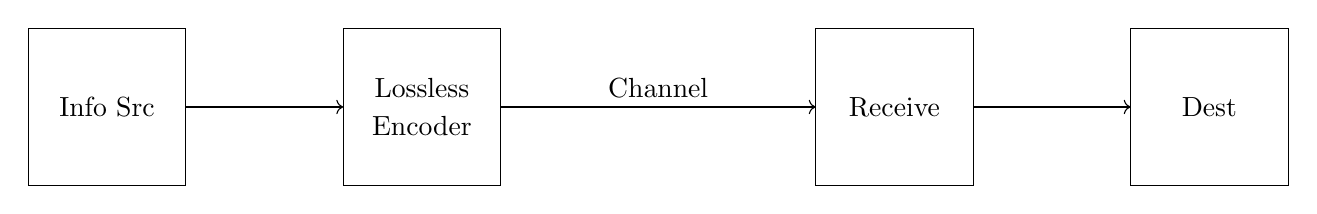
\begin{tikzpicture}[scale=2]
\draw[black] (-4, 0) rectangle (-3, 1) (-2, 0) rectangle (-1, 1) (1, 0) rectangle (2, 1) (3, 0) rectangle (4, 1);
\draw[->] (-3, 0.5) -- (-2, 0.5);
\draw[->] (-1, 0.5) -- (1, 0.5);
\draw[->] (2, 0.5) -- (3, 0.5);
\draw (-3.5, 0.5) node[anchor=center] {Info Src}
    (-1.5, 0.5) node[above] {Lossless}
    (-1.5, 0.5) node[below] {Encoder}
    (1.5, 0.5) node[anchor=center] {Receive}
    (3.5, 0.5) node[anchor=center] {Dest}
    (0, 0.5) node[anchor=south] {Channel};
\end{tikzpicture}

Think of waveforms. Let us have three different kinds of waveforms we can send, corresponding to 0, 1, 2. But, the channel will add noise to these waves. Let the input to the channel be $X$ and the output be $Y$:
\[P(Y|X=x_1),P(Y|X=x_2),P(Y|X=x_3).\]
\begin{enumerate}
    \item Send something through the channel. Before it comes out of the pipe, I ask how surprised you would be if $X=x$ was sent, this would be
    \[\log\frac{1}{p(x)}.\]
    \item When it comes out, we find that $Y=y.$ Now, how surprised are you? this would be
    \[\log\frac{1}{p(x|y)}.\]
    \item The information you gain from seeing $y$ come out is 
    \[\log\frac{1}{p(X=x)}-\log\frac{1}{P(X=x|Y=y)}.\]
    \item In the long run,
    \begin{align*}&E_{x,y}\left[\log\frac{1}{P(X=x)}-\log\frac{1}{P(X=x,Y=y)}\right]\\&\quad =\sum p(x,y)\log\frac{p(x|y)}{p(x)}\\&\quad =\sum p(x,y)\log\left(\frac{p(x|y)}{p(x)}\frac{p(y)}{p(y)}\right)=I(X;Y).\end{align*}
\end{enumerate}
\[C(Y|X)\] is the notation for channel capacity, and it is defined by the maximum of $I(X;Y)$ over  $X$ and $Y.$



\section{Channels}
\subsection{Channel Capacity}
Recall that
\[C(Y|X)=\sup\{I(X;Y)\}_{X,Y}.\]

\paragraph{Example 1}
Noiseless Binary Channel
\[p:0\to 0\qquad (1-p):1\to 1\]

\[I(X;Y)=\sum\sum p(x,y)\log\frac{p(x,y)}{p(x)p(y)}=H(p),\]
\[\therefore C(X|Y)=\sup\{h(p):p\in[0,1]\}=1\si{bit},\]
when $X$ is a uniform distribution.

\paragraph{Example 2}
Noisy channel with non-overlapping outputs.

\begin{figure}[h!]
    \centering
    \begin{tabular}{|c|c|}
    \hline 
    X & Y \\
    \hline
     \multirow{2}{*}{1} & 1 $(p=1/2)$ \\
     \cline{2-2}
     & 2 $(p=1/2)$\\
     \hline
     \multirow{2}{*}{2} & 3 $(p=1/3)$ \\
     \cline{2-2}
     & 4 $(p=2/3)$  \\
     \hline
\end{tabular}
\end{figure}
\[I(X;Y)=\sum\sum p(x,y)\log\frac{p(x,y)}{p(x)p(y)}=H(X)-H(X|Y)=H(X)=H(p)\] because $H(X|Y)=0$ since they are disjoint, and thus
\[C(Y|X)=1\si{bit}.\]

\paragraph{Example 3}

Let $A\to A$ with probability $1/2$ and $B$ with probability $1/2,$ etc. to $Z\to Z_{0.5}, A_{0.5}$

We have
\begin{align*}
I(X;Y)&=\sum\sum p(x,y)\log\frac{p(x,y)}{p(x)p(y)}\\&=\sum\sum_{x=y}p(x,y)\log\frac{p(x,y)}{p(x)p(y)}+\\&\sum\sum_{x+1\equiv y\pmod{26}}p(x,y)\log\frac{p(x,y)}{p(x)p(y)}\\&=\sum\sum_{x=y}\frac{1}{2}p_i\log\frac{p_i/2}{p_i\cdot (p_i/2+p_{i-1}/2)}\\&+\sum\sum_{x+1\equiv y\pmod{26}}\frac{1}{2}p_i\log\frac{p_i/2}{p_i\cdot (p_i/2+p_{i-1}/2)}\\&=H(Y)-1.
\end{align*}

Alternatively,
\[I(X;Y)=H(Y)-H(Y|X)=H(Y)-1,\]
since it's just a 50/50 given $X.$ But, $H(Y)\le\log(26),$ and if $X$ is uniform, $Y$ must be as well, so this is attainable.

\bigskip
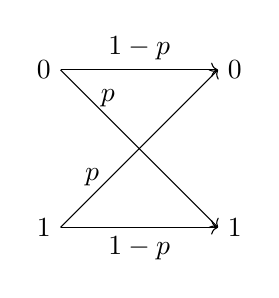
\begin{tikzpicture}[scale=2.0]
    \draw (0,0) node[anchor=east] {1} (0,1) node[anchor=east] {0} (1,0) node[anchor=west] {1} (1,1) node[anchor=west] {0};
    \draw[->] (0, 0) -- node[pos=0.2,above] {$p$} (1,1);
    \draw[->] (0, 0) -- node[below] {$1-p$} (1,0);
    \draw[->] (0, 1) -- node[pos=0.3,above] {$p$} (1,0);
    \draw[->] (0, 1) -- node[above] {$1-p$} (1,1);
\end{tikzpicture}

\paragraph{Example 4}
\[I(X;Y)=H(Y)-H(Y|X)\le 1-H(Y|X)=1-H(p),\]
which is achieved when $Y$ and $X$ are both uniform.
Alternatively,
\begin{align*}I(X;Y)&=\sum_x\sum_y p(x,y)\log\frac{p(x,y)}{p(x)p(y)}\\&=q(1-p)\log\frac{q(1-p)}{q(q(1-p)+(1-q)p)}\\&\quad +qp\log\frac{qp}{q(qp+(1-q)(1-p))}\\&\quad +(1-q)p\log\frac{(1-q)p}{(1-q)(q(1-p)+(1-q)p)}\\&\quad +(1-q)(1-p)\log\frac{(1-q)(1-p)}{(1-q)(qp+(1-q)(1-p))}\\&=H(\text{some binary distribution})-H(p)\\&\le \boxed{1-H(p)}.\end{align*}



\subsection{BEC/Symmetric Channels 11.7.2024}

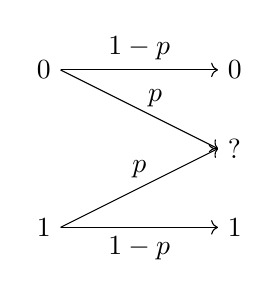
\begin{tikzpicture}[scale=2.0]
    \draw (0,0) node[anchor=east] {1} (0,1) node[anchor=east] {0} (1,0) node[anchor=west] {1} (1,1) node[anchor=west] {0} (1, 0.5) node[anchor=west] {?};
    \draw[->] (0, 0) -- node[pos=0.5,above] {$p$} (1,0.5);
    \draw[->] (0, 0) -- node[below] {$1-p$} (1,0);
    \draw[->] (0, 1) -- node[pos=0.6,above] {$p$} (1,0.5);
    \draw[->] (0, 1) -- node[above] {$1-p$} (1,1);
\end{tikzpicture}

\begin{align*}I(X;Y)&=\sum_{x,y}p(x,y)\log\frac{p(x,y)}{p(x)p(y)}\\&=q(1-\alpha)\log\frac{q(1-\alpha)}{q^2(1-\alpha)}+q\alpha\log\frac{q\alpha}{q\alpha}+(1-q)\alpha\log\frac{(1-q)\alpha}{(1-q)\alpha}+(1-q)(1-\alpha)\log\frac{(1-q)(1-\alpha)}{(1-q)^2(1-\alpha)}\\&=(1-\alpha)q\log\frac{1}{q}+(1-\alpha)\log\frac{1}{(1-q)}=(1-\alpha)H(q)\le 1-\alpha,\end{align*} which occurs when $X$ is uniform. 

You might be tempted to do the following:
\[C=\sup\{I(X;Y)\}=\sup\{H(Y)-H(Y|X)\}=\sup\{H(Y)-H(\alpha)\}\ne\log3-H(\alpha),\]
since we can't guarantee to create a uniform distribution on the right.

Instead, try the other way:
\[C=\sup\{H(X)-H(X|Y)\}=\sup\{1-H(X|Y=?)P(?)\}=1-\alpha,\] which occurs when $X$ is uniform.



\subsubsection{Gaussian Channel}
This is a continuous channel, so we will be using differential entropy. This channel adds random noise to the input, and this noise is normally distributed. For input $X$, output $Y = X + Z$ where $Z \sim N(\mu, \sigma^2)$. Without loss of generality, assume $\mu = 0$.

Constraint: ``cost'' of sending $X$ is $\text{Var}[X] = \sigma_x^2$, otherwise we can send infinite information or something.

Since this must be at best independent, 
\[\sigma_y^2\le\sigma_x^2+\sigma_z^2\]
From the entropy of a Gaussian, and the fact that it maximizes differential entropy:
\begin{align*}h(Y) &\le \frac{1}{2} \log_2 2 \pi e \sigma_y^2 \\
 &\le \frac{1}{2} \log_2 2 \pi e (\sigma_x^2 + \sigma_z^2).
\end{align*}
Because $Z$ and $X$ are independent (i.e. $h(Z|X) = h(Z)$):
\[I(X;Y)=h(Y)-h(Y|X)=h(Y)-h(Z)\le\frac{1}{2}\log 2\pi\frac{\sigma_x^2+\sigma_z^2}{\sigma_z^2}.\]


\paragraph{Symmetric Channels}
We call a channel symmetric if $p(y|x)$ is symmetric as such:

The matrix of $p(y|x)$ is:
\[\begin{bmatrix}
    0.3&0.2&0.5\\
    0.5&0.3&0.2\\
    0.2&0.5&0.3
\end{bmatrix}.\]

The entry in the $x^\text{th}$ row and $y^\text{th}$ column is the conditional probability $p(y|x)$ that $y$ is received given $x$ is sent. Since all the rows and columns are permutations of each other, we call it symmetric (even though the matrix isn't).

Consider
\[Y=(X+Z)\mod{c},\]
where $X$ and $Z$ are some distributions on $\mathbb{Z}/c\mathbb{Z}$ and are independent.

Given 
\[p(y|x):\begin{bmatrix}
    0.3&0.2&0.5\\
    0.5&0.3&0.2\\
    0.2&0.5&0.3
\end{bmatrix},\]
find $C(Y|X).$
\[I(X;Y)=H(Y)-H(Y|X)=H(Y)-H(\{0.3,0.2,0.5\})\le \log 3-H(\{0.3,0.2,0.5\}).\]
If input is uniform, then $Y$ is uniform as well, so this works.


\paragraph{Computer Architecture}
Properties of Channel Capacity:

\begin{enumerate}
    \item Because $I(X;Y)\ge 0$ \[C(Y|X)\ge 0\]
    \item Because $I(X;Y)\le H(X),H(Y)$ \[C\le \log|\mathscr{X}| \qquad\text{and}\qquad C\le\log|\mathscr{Y}|\]
    \item $I(X;Y)$ is continuous and concave on $p(x).$
\end{enumerate}


\subsection{Comp Arch. 101}


% \begin{tikzpicture}
% % Circuit style
% \ctikzset{
% 	logic ports=ieee,
% 	logic ports/scale=0.8,
% 	logic ports/fill=lightgray
% }
% % Logic ports
% \node[or port] (ORa) at (0,0){};
% \node[not port] (Noa) at (0,-2){};
% \node[or port] (ORb) at (0,-4){};
% \node[not port] (Nob) at (2.5,0){};
% \node[and port] (ANDa) at (2.5,-3){};
% \node[or port] (ORc) at (5,-1.5){};
% % Connection
% \draw (ORa.out) -- (Nob.in);
% \draw (Noa.out) -| (ANDa.in 1);
% \draw (ORb.out) -| (ANDa.in 2);
% \draw (ANDa.out) -|  (ORc.in 2);
% \draw (Nob.out) -| (ORc.in 1);
% \draw (ORc.out) -- ++(1,0) node[near end,above]{Out};
% \draw (ORa.in 1) -- ++(-1.5,0)node[left](In1){In1};
% \draw (ORb.in 2) -- ++(-1.5,0)node[left](In3){In3};
% % Jump crossing element
% \node at (ORa.in 2)
% [
% 	below,
% 	jump crossing,
% 	rotate=-90,
% 	scale=1.3
% ](X){};
% \draw (Noa.in) -| (X.east)
% 	(X.west) to[short,-*] (X.west |- ORa.in 1); 
% \draw ($ (In1) !.5! (In3) $) node[]{In2}
% 	++ (0.4,0) to[short,-*] ++(0.5,0) coordinate(a)
% 	|- (X.south) (a) |- (ORb.in 1);
% \end{tikzpicture}

\paragraph{AND gate:} $z = x\wedge y = x \cdot y = x \text{ AND } y$

 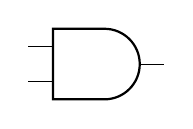
\begin{tikzpicture}
% % Circuit style
 \ctikzset{
 	logic ports=ieee,
 	logic ports/scale=0.8
 }
% % Logic ports
 \node[and port] (ANDa) at (0,0){};
\end{tikzpicture}
\begin{tabular}{c|c|c}
$x(t)$&$y(t)$&$z(t)$\\
\hline
0&0&0\\
0&1&0\\
1&0&0\\
1&1&1
    
\end{tabular}

\paragraph{OR gate:} $z = x \vee y = x + y = x \text{ OR } y$

 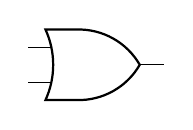
\begin{tikzpicture}
% % Circuit style
 \ctikzset{
 	logic ports=ieee,
 	logic ports/scale=0.8
 }
% % Logic ports
 \node[or port] (ORa) at (0,0){};
\end{tikzpicture}
\begin{tabular}{c|c|c}
$x(t)$&$y(t)$&$z(t)$\\
\hline
0&0&0\\
0&1&1\\
1&0&1\\
1&1&1
    
\end{tabular}

\paragraph{NOT gate:} $y = \text{NOT } x = \bar x = \sim x$

 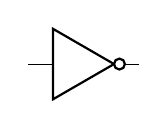
\begin{tikzpicture}
% % Circuit style
 \ctikzset{
 	logic ports=ieee,
 	logic ports/scale=0.8
 }
% % Logic ports
 \node[not port] (NOTa) at (0,0){};
\end{tikzpicture}
\begin{tabular}{c|c}
$x(t)$&$y(t)$\\
\hline
0&1\\
1&0    
\end{tabular}

\paragraph{Delay/Flipflop:} $y=Dx$ 
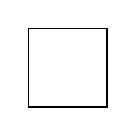
\begin{tikzpicture}
    \draw (0,0) rectangle (1,1);
\end{tikzpicture}
delays output by 1 clock cycle. Only element with a notion of memory. Everything else is memoryless/instantaneous.

Ignore this: \[D = e^{\fdiffn{}{x}}\]

\begin{tabular}{c|c}
$x(t)$&$y(t+1)$\\
\hline
0&0\\
1&1    
\end{tabular}
\paragraph{Sticky Bit:}
As long as you see 0, you will output 0. Once you see a 1 you output a 1 and then it remains at 1 forever. $z[t+1] = z[t] \vee x[t]$

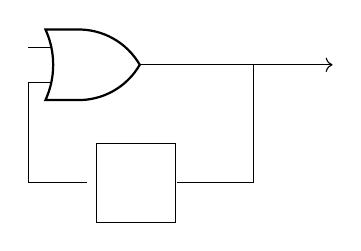
\begin{tikzpicture}
% % Circuit style
 \ctikzset{
 	logic ports=ieee,
 	logic ports/scale=0.8
 }
% % Logic ports
 \node[or port] (OR) at (0,0){};
 % draw square here
 \draw (0,-2) rectangle (1,-1) (0.9,-1.5) node(delayin){} (0, -1.5) node(delayout) {};
 \draw (OR.out) -- (2,0) -- (2,-1.5) -- (delayin);
 \draw (delayout) -| (OR.in 2);
 \draw[->] (2,0) -- (3,0);
\end{tikzpicture}

\paragraph{Toggle Bit}
When you see a zero, output the same bit as before, but flip it if you see a 1.
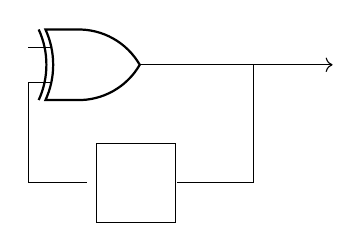
\begin{tikzpicture}
% % Circuit style
 \ctikzset{
 	logic ports=ieee,
 	logic ports/scale=0.8
 }
% % Logic ports
 \node[xor port] (XOR) at (0,0){};
 % draw square here
 \draw (0,-2) rectangle (1,-1) (0.9,-1.5) node(delayin){} (0, -1.5) node(delayout) {};
 \draw (XOR.out) -- (2,0) -- (2,-1.5) -- (delayin);
 \draw (delayout) -| (XOR.in 2);
 \draw[->] (2,0) -- (3,0);
\end{tikzpicture}
Make sure you understand why these work.

Parallel AND: $k$ bits going to each input, $k$ bits outputted, each correspond bit is ANDed, so
$11000$ AND $01100$ is $01000.$ 

\begin{lstlisting}
    uncurry (&&) <$> zip a b
\end{lstlisting}

Aggregate AND: everything ANDed together. 

\begin{lstlisting}
    foldr (&&) True $ (a++b)
    all id $ (a++b)
\end{lstlisting}

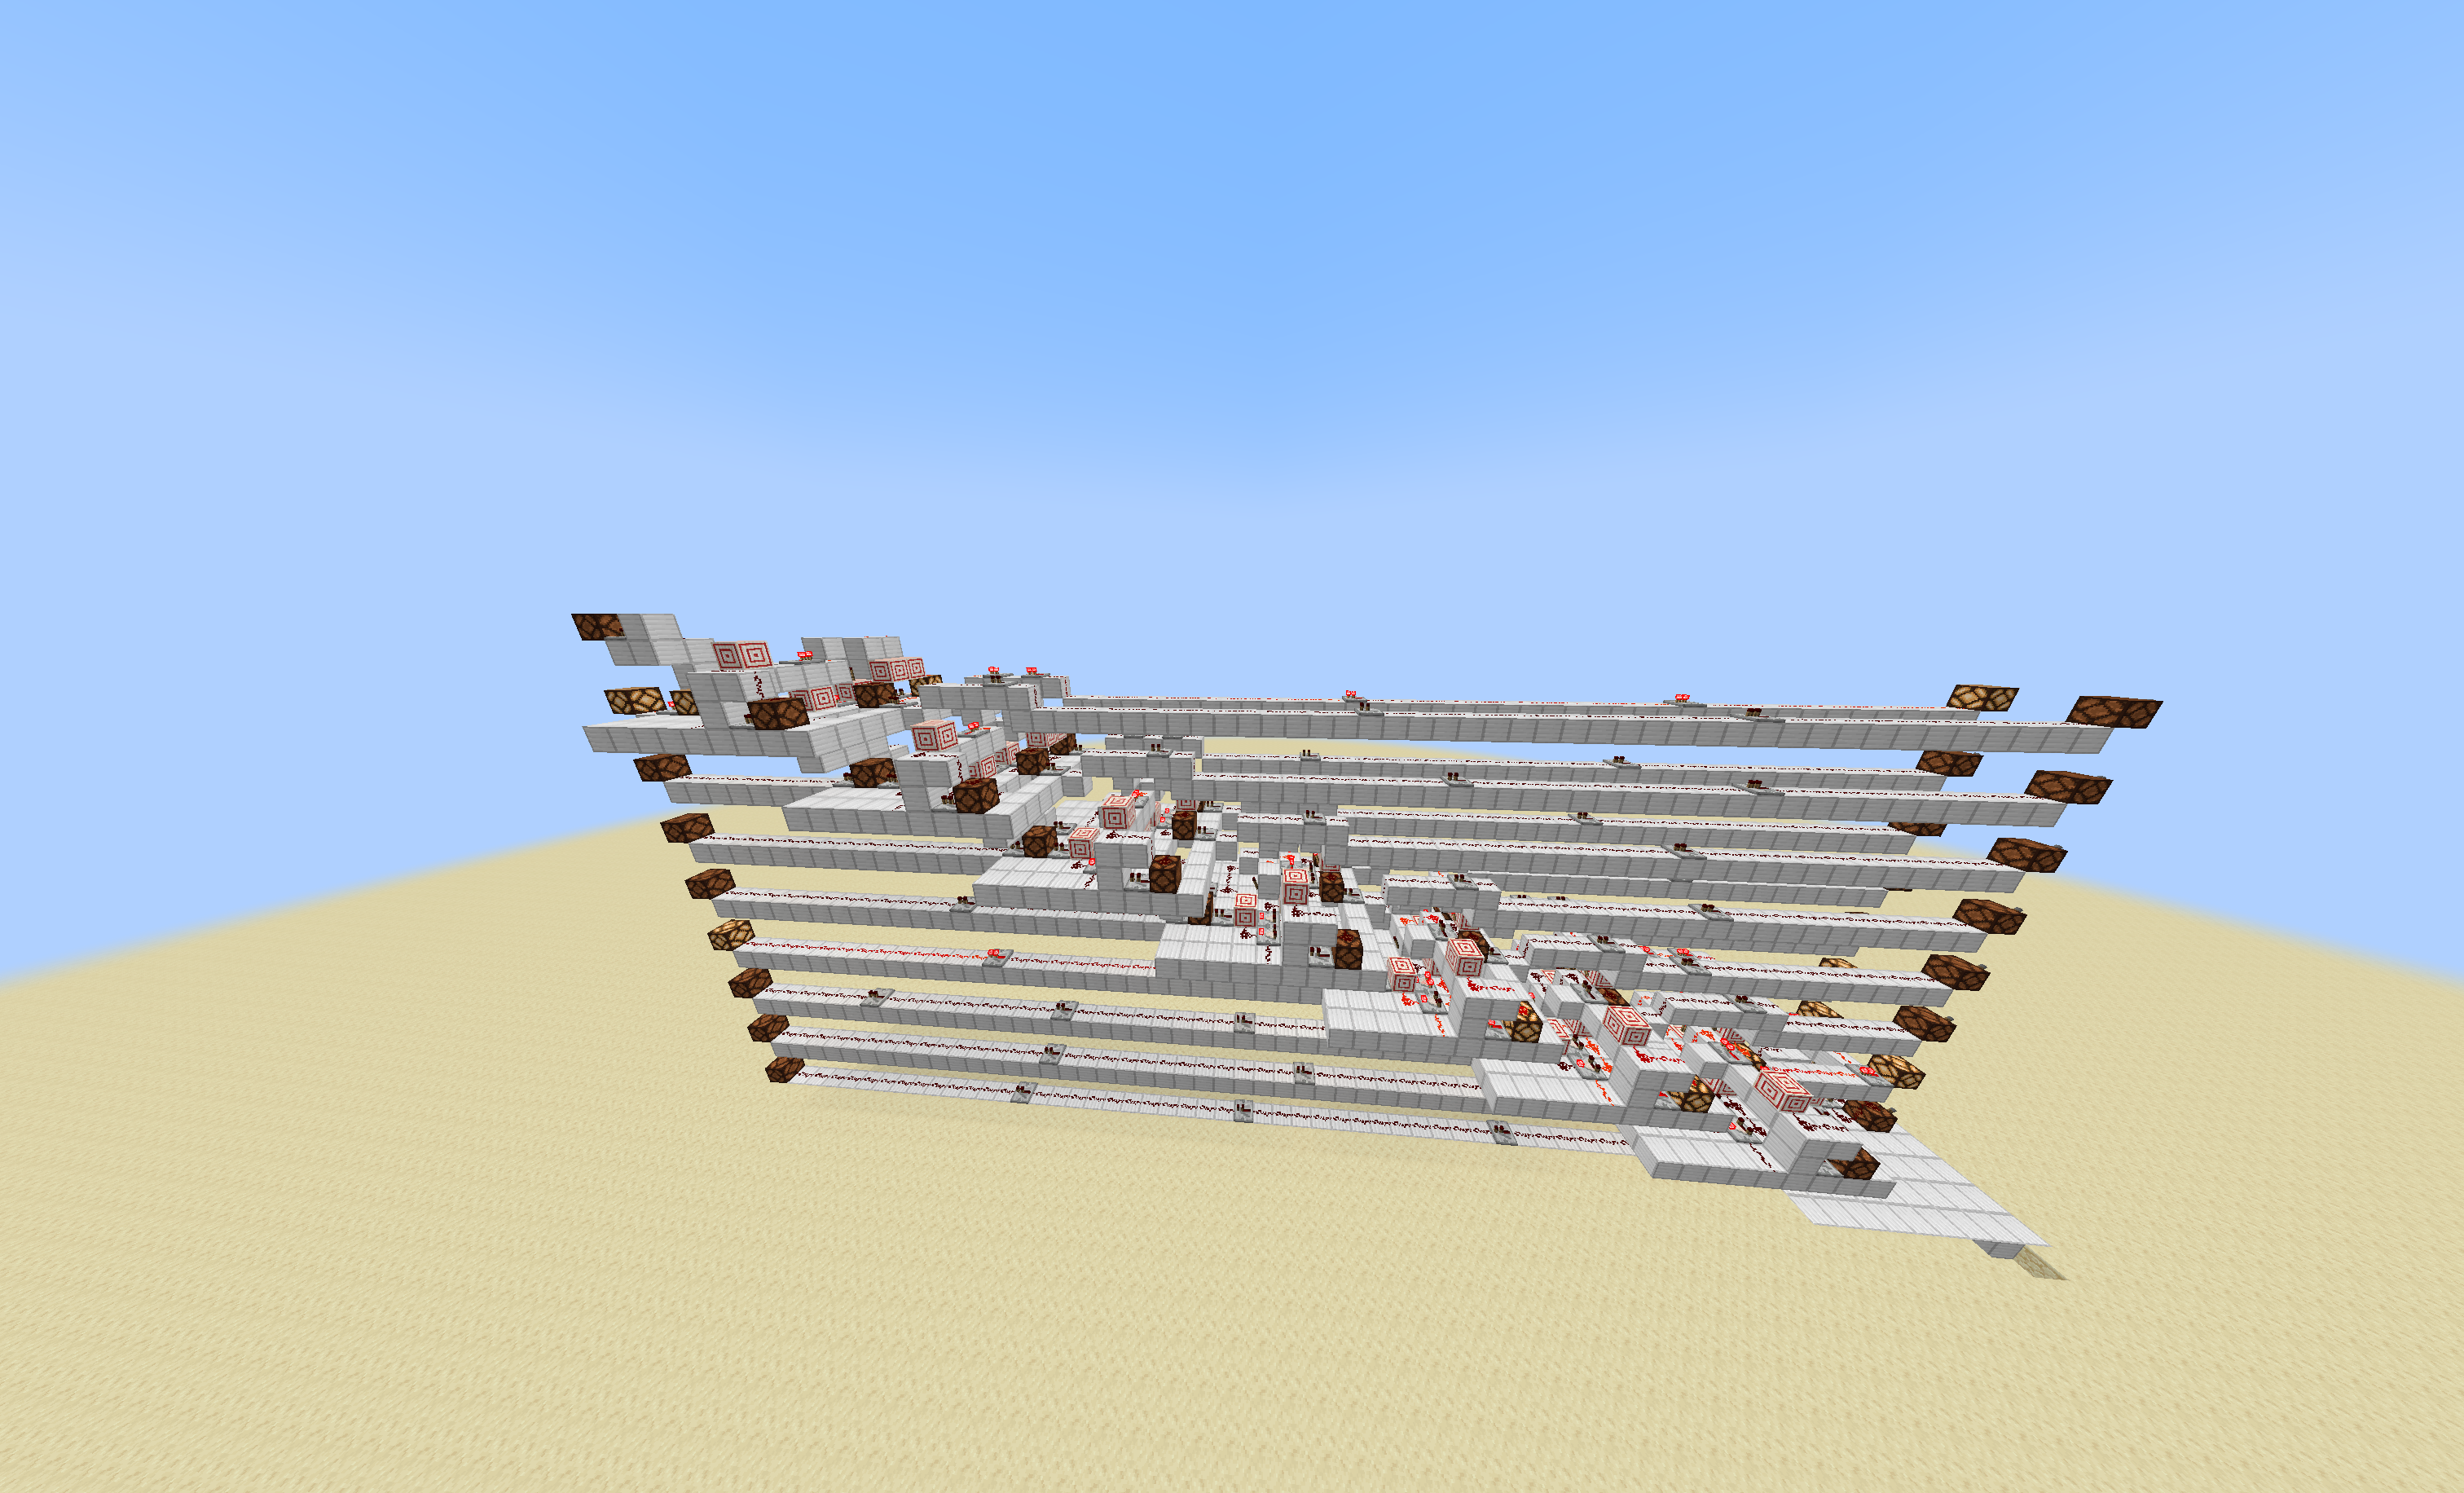
\includegraphics[width=\textwidth]{8bitadder.png}
(Not to be confused with the snake)

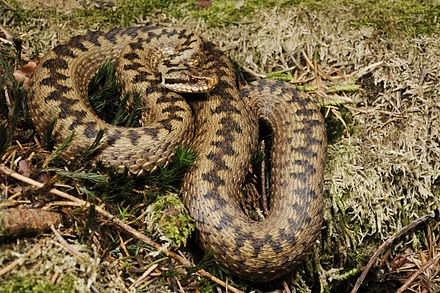
\includegraphics[width=0.5\textwidth]{adder.jpg}
$k$-bit adder:
Each layer takes in $x_i,y_i,c_i$ and outputs $z_i,c_{i+1}$
We have


\begin{tabular}{c|c|c||c|c}
$x_i(t)$&$y_i(t)$&$c_i(t)$&$z_i(t)$&$c_{i+1}(t)$\\
\hline
0&0&0&0&0\\
0&0&1&1&0\\
0&1&0&1&0\\
0&1&1&0&1\\
1&0&0&1&0\\
1&0&1&0&0\\
1&1&0&0&1\\
1&1&1&1&1
\end{tabular}

So,
\[z_i(t)=\bar{x_i}\bar{y_i}c_i+\bar{x_i}y_i\bar{c_i}+x_i\bar{y_i}\bar{c_i}+x_iy_ic_i.\]

\paragraph{Theorem}
Given $f:\mathbb{F}_2^k\to\mathbb{F}_2^l,$ we can find some memoryless circuit with that does this. This can be done only with AND, OR, and NOT gates.

Define a stream $stream(\mathbb{F}_2^k)$ to be the set of infinite sequences, each element of which is a $k$-bit block. Then for every function
\[f:stream(\mathbb{F}_2^k)\to stream(\mathbb{F}_2^l),\] we can build a circuit that implements $f$ using only AND, OR, NOT, FLIPFLOPS, provided that only a finite amount of memory is necessary.
\subsection{Hamming Codes and Shift Registers (11.13.2024)}
Recall: Source codes try to compress the input to maximize efficiency, but channel codes add redundancy to be able to correct for noise.

There are $n$ basis waveforms, which are combined through the channel. The waveforms are sent at different times to be encodable and decodable (TDM, Time Division Multiplexing). You could also split them in frequency (FDM, Frequency Division Multiplexing).

However, we don't care about this. We will only look at the digital channel coding. 

\subsubsection{Channel Coding}
\paragraph{Example}
$k$-bit message: $11001.$

Code: 000 111 111 000 000 111
$n=3k$

\smallskip
\begin{tabular}{|c|c|c|}
    \hline
    $k$&$n$&$e$\\
    \hline
    arbitrary&$3k$&1 per block of 3 \\
    \hline
\end{tabular}.
\paragraph{Example 2}
$k$ bits and a parity bit at the end: counts the number of $1$'s modulo 2 (even or odd number of 1's correspond to a 0 or 1).

\smallskip
\begin{tabular}{|c|c|c|}
    \hline
    $k$&$n$&$e$\\
    \hline
    arbitrary&$k+1$&Only error identification, but not error correction \\
    \hline
\end{tabular}


\paragraph{Example 3}
Double Parity:

\smallskip
\begin{tabular}{c|c|c|}
    \multicolumn{1}{c}{} & \multicolumn{1}{c}{$k_2$} & \multicolumn{1}{c}{parity} \\
    \cline{2-3}
    $k_1$ & k bits & \\
    \cline{2-3}
    parity & & x \\
    \cline{2-3}
\end{tabular}

\bigskip
\begin{tabular}{|c|c|c|}
    \hline
    $k$&$n$&$e$\\
    \hline
    $k_1k_2$&$k_1k_2+k_1+k_2$&1 \\
    \hline
\end{tabular}
\subsubsection{Hamming Codes}
A good code has a high $e$ and a low $n$
\begin{tabular}{|c|c|c|}
\hline
    $k$&$n$&$e$ \\
    \hline
    4&7&1 \\
    \hline
\end{tabular}


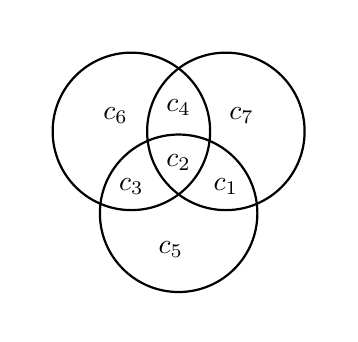
\begin{tikzpicture}[thick]
        % \draw (2.7,-2.54) rectangle (-1.5,1.5) node[below right] {};
        \draw (0,0) circle (1) node[above,shift={(0,1)}] {};
        \draw (1.2,0) circle (1) node[above,shift={(0,1)}] {};
        \draw (.6,-1.04) circle (1) node[shift={(1.1,-.6)}] {};

        \node at (.6,-.4) {$c_2$};
        \node at (1.2,-.7) {$c_1$};
        \node at (0,-.7) {$c_3$};
        \node at (1.4,.2) {$c_7$};
        \node at (.6,.3) {$c_4$};
        \node at (-.2,.2) {$c_6$};
        \node at (2.2,-1.2) {};
        \node at (-1,-2.2) {};
        \node at (2.4,1.2) {};
        \node at (.5,-1.5) {$c_5$};
        \node at (1,-1.4) {};
        \node at (-1.2,-1.5) {};
\end{tikzpicture}
(Sorry this is upside down from what we did in class but I can't find a venn diagram that is facing the right way online)
The message is $c_1c_2c_3c_4,$ and the output is $c_1c_2c_3c_4c_5c_6c_7,$
where
\[c_5=\text{parity of }c_1c_2c_3=c_1\oplus c_2\oplus c_3\]
\[c_6=c_2\oplus c_3\oplus c_4\]
\[c_7=c_1\oplus c_2\oplus c_4\]

\begin{enumerate}
\item $0101\to0101100$
\item $1100\to1100010$
\item $0000\to0000000$
\item $1111\to1111111$
\end{enumerate}
To decode, we put it back on the venn diagram and check if it works.

For 0111010, we have

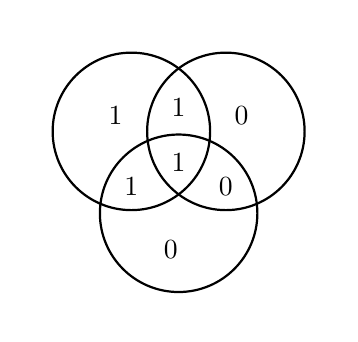
\begin{tikzpicture}[thick]
        % \draw (2.7,-2.54) rectangle (-1.5,1.5) node[below right] {};
        \draw (0,0) circle (1) node[above,shift={(0,1)}] {};
        \draw (1.2,0) circle (1) node[above,shift={(0,1)}] {};
        \draw (.6,-1.04) circle (1) node[shift={(1.1,-.6)}] {};

        \node at (.6,-.4) {$1$};
        \node at (1.2,-.7) {$0$};
        \node at (0,-.7) {$1$};
        \node at (1.4,.2) {$0$};
        \node at (.6,.3) {$1$};
        \node at (-.2,.2) {$1$};
        \node at (2.2,-1.2) {};
        \node at (-1,-2.2) {};
        \node at (2.4,1.2) {};
        \node at (.5,-1.5) {$0$};
        \node at (1,-1.4) {};
        \node at (-1.2,-1.5) {};
\end{tikzpicture},

which checks out.
However, if we get 0100100, we have

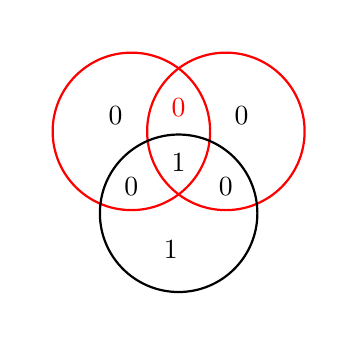
\begin{tikzpicture}[thick]
        % \draw (2.7,-2.54) rectangle (-1.5,1.5) node[below right] {};
        \draw[red] (0,0) circle (1) node[above,shift={(0,1)}] {};
        \draw[red] (1.2,0) circle (1) node[above,shift={(0,1)}] {};
        \draw (.6,-1.04) circle (1) node[shift={(1.1,-.6)}] {};

        \node at (.6,-.4) {$1$};
        \node at (1.2,-.7) {$0$};
        \node at (0,-.7) {$0$};
        \node at (1.4,.2) {$0$};
        \node[red] at (.6,.3) {$0$};
        \node at (-.2,.2) {$0$};
        \node at (2.2,-1.2) {};
        \node at (-1,-2.2) {};
        \node at (2.4,1.2) {};
        \node at (.5,-1.5) {$1$};
        \node at (1,-1.4) {};
        \node at (-1.2,-1.5) {};
\end{tikzpicture}

which has only two wrong circles. The only member of the wrong circles that isn't a member of any right circles is $c_4,$ so the correct message must be 0101.

Although we can draw Hamming codes easily with venn diagrams, in general codes are too complicated to do this. So we need shift registers.

\subsubsection{Shift Registers}
What is a shift register? A SR is a circuit that forms an important building block in both encoders and decoders. It looks like this:

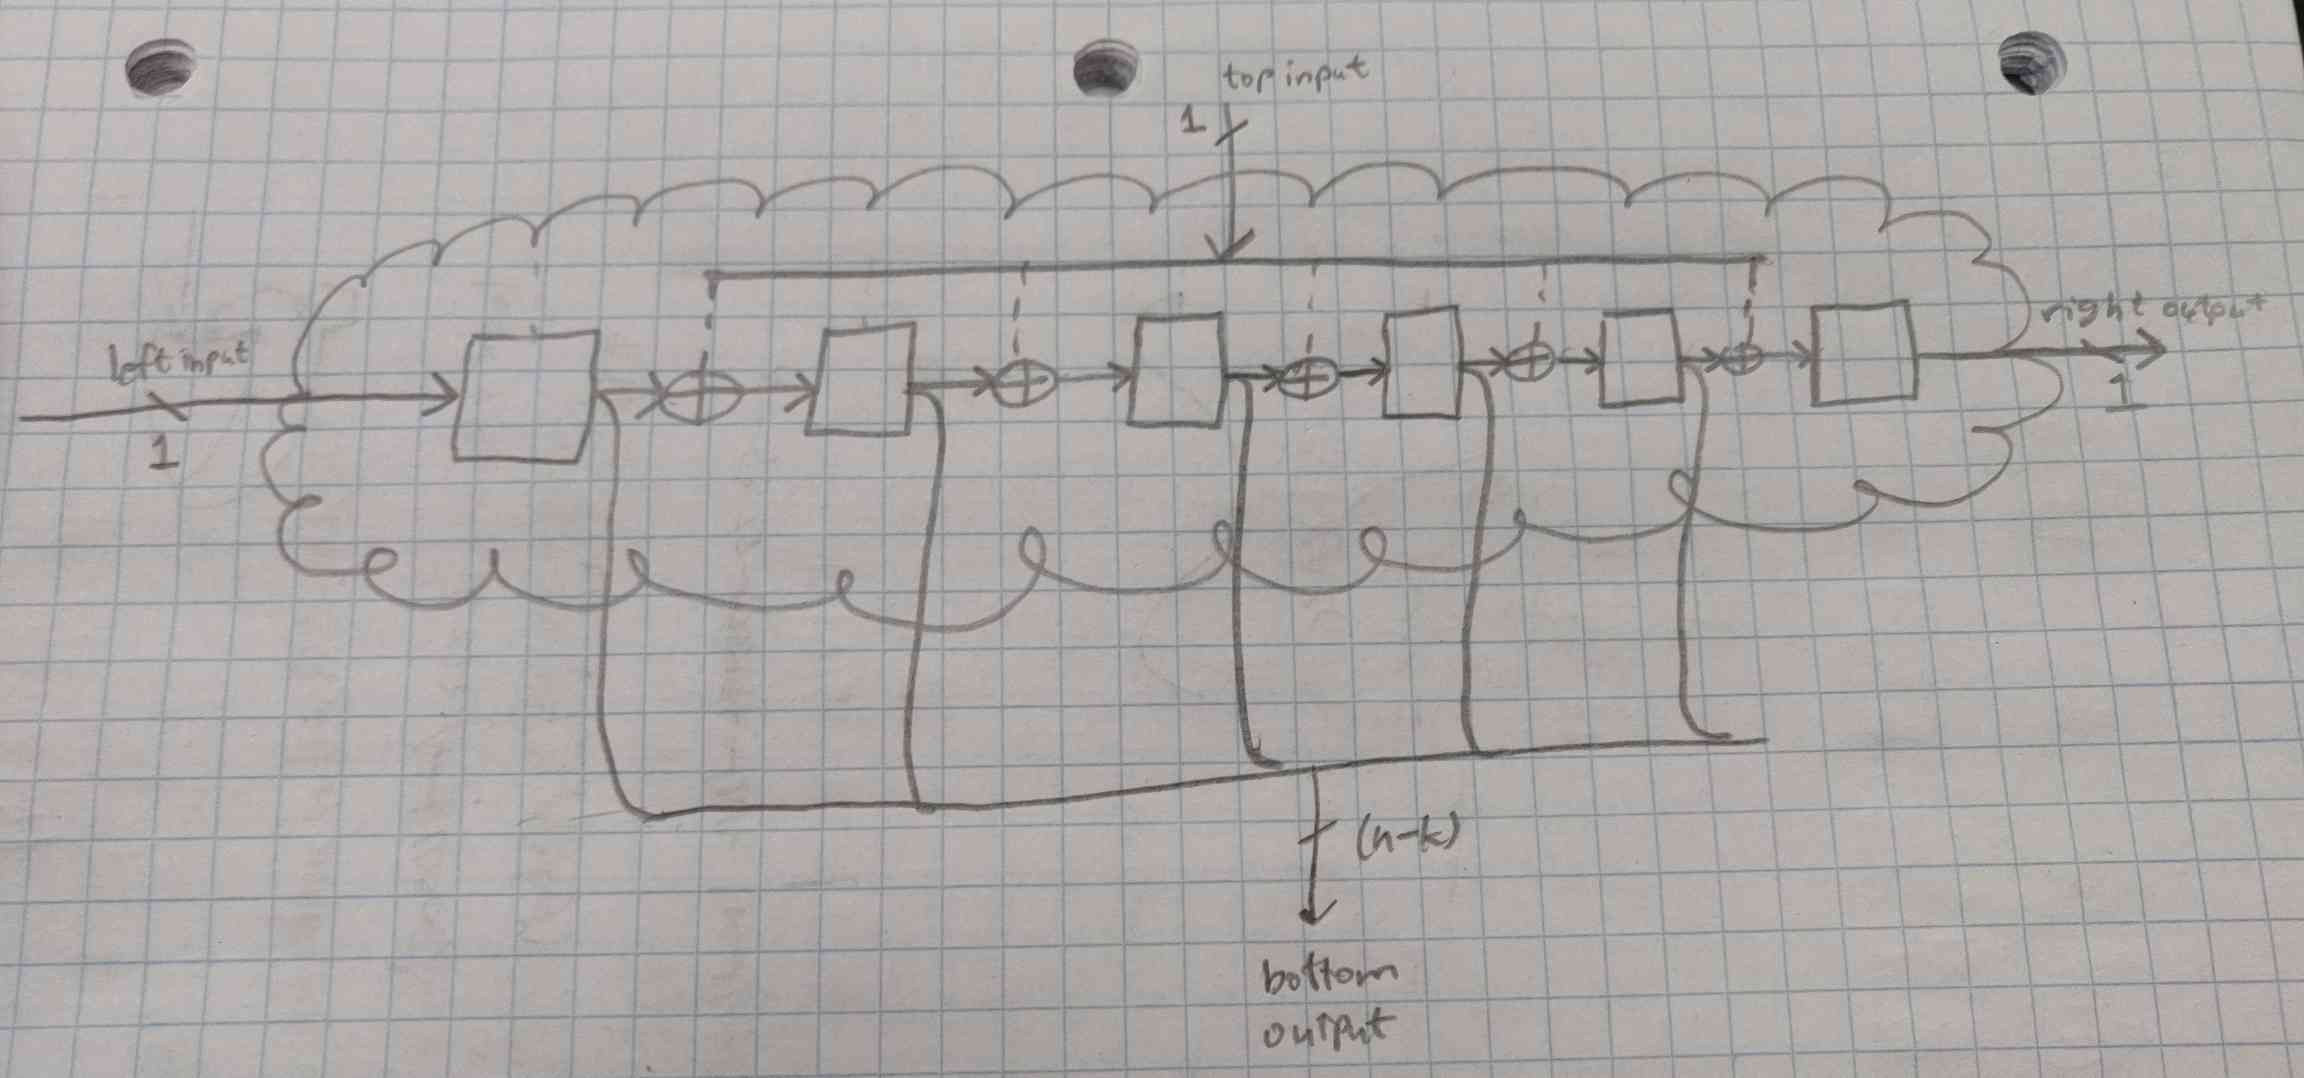
\includegraphics[width=\textwidth]{sr.jpg}
The length of the SR is arbitrary. The dashed lines do not have to be connected, and using different patterns of the connections produce different codes. We say that the SR has a ``tap'' in position $i$ if the $i$th XOR is connected.

For Hamming codes:


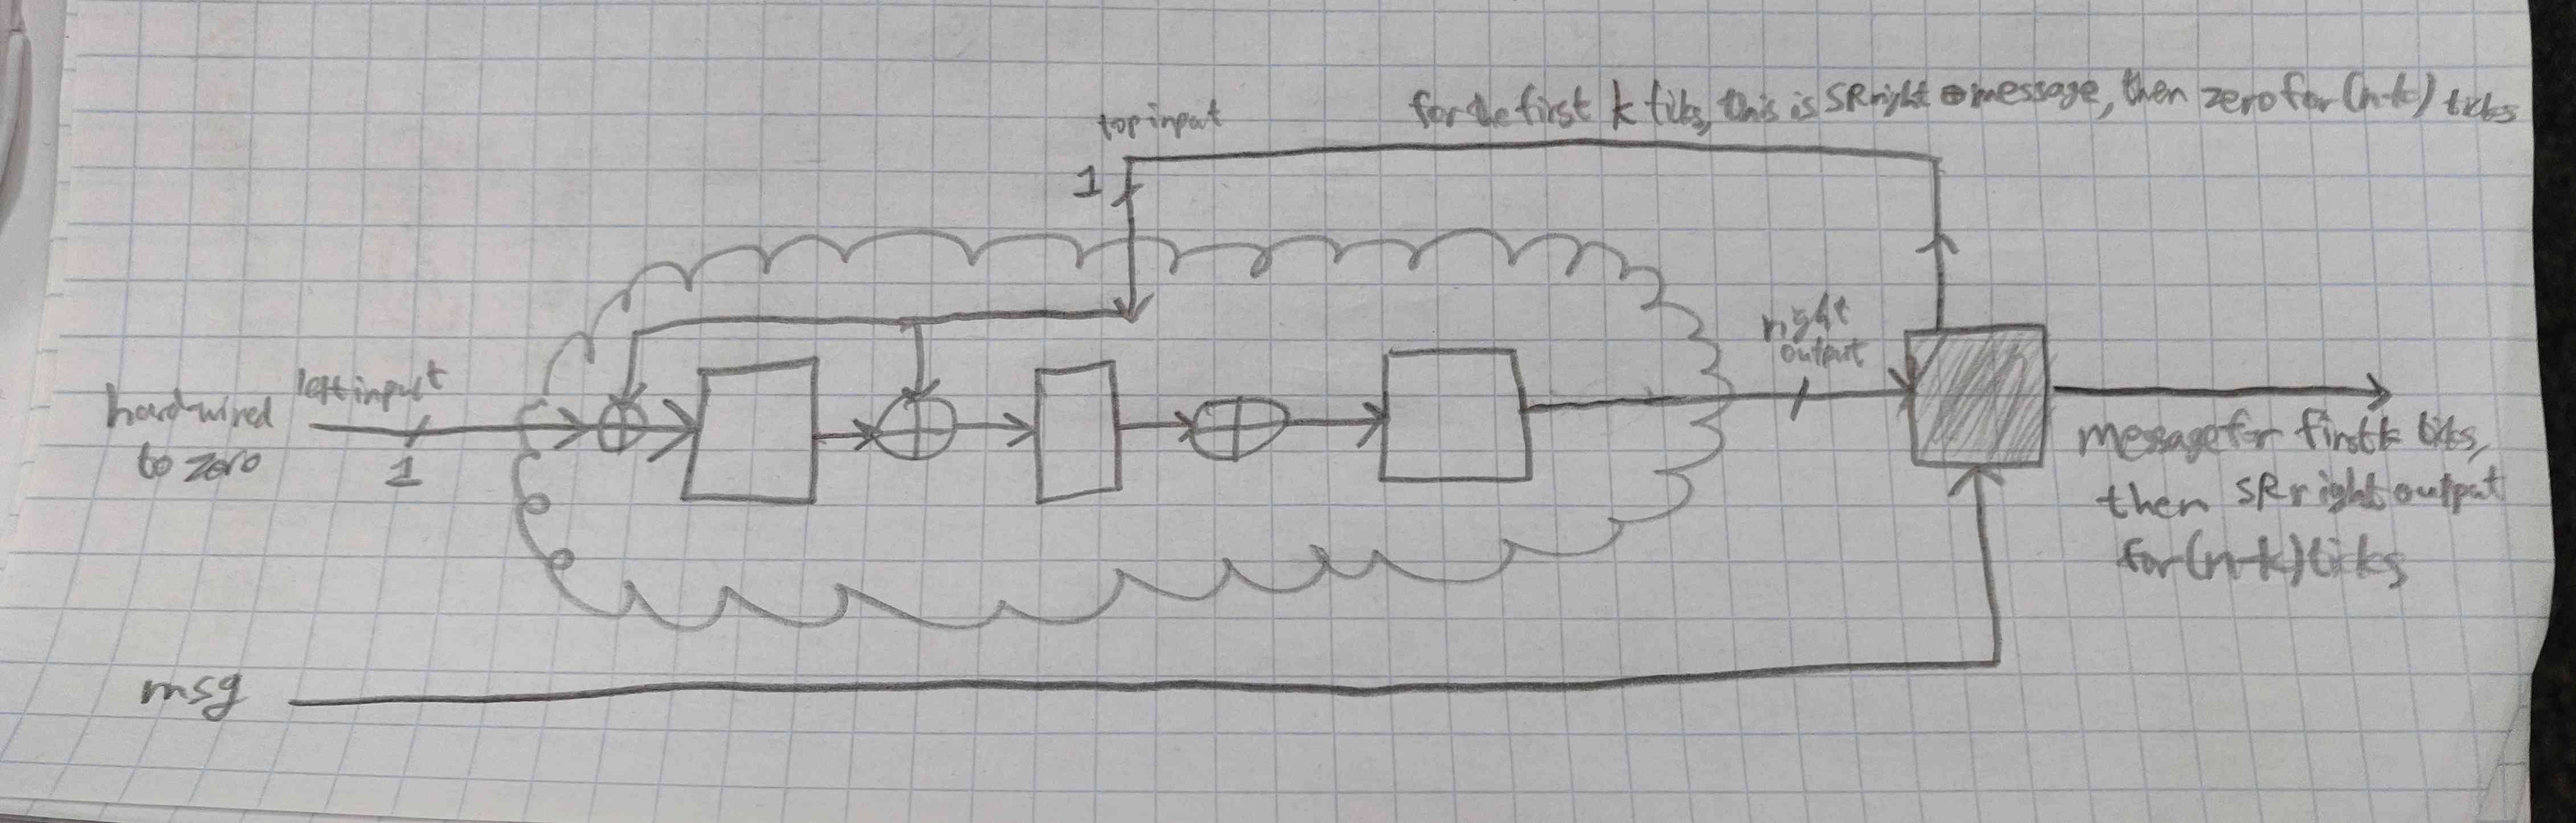
\includegraphics[width=\textwidth]{srHamming.jpg}
Note that the third XOR isn't tapped (so it doesn't do anything)
SR out means the outputs of the internal FlipFlops to keep track of the state throughout the process (SR bottom). For clarity, clock ticks happen between steps, so SROut denotes the state of the system before the step has been propagated.

Our message is $1010,$ read from right to left, i.e. the order read will be $0,1,0,1,$ and then after that it will read zeros only.



\begin{tabular}{|c|c|c||c|c|}
    \hline
     Step & SR Out (3 bits) & Message (1 bit) & SR In/Top (1 bit) & Codeword (1 bit)  \\
     \hline
     1& 000&0& 0&0\\
     2& 000 & 1&1&1\\
     3& 110 & 0&0&0\\
     4& 011 & 1&0&1\\
     5& 001 & 0&0&1\\
     6& 000 & 0&0&0\\
     7& 000 & 0&0&0\\
     \hline
\end{tabular}



\subsection{Hamming Encoding and Decoding (11.15.2024)}
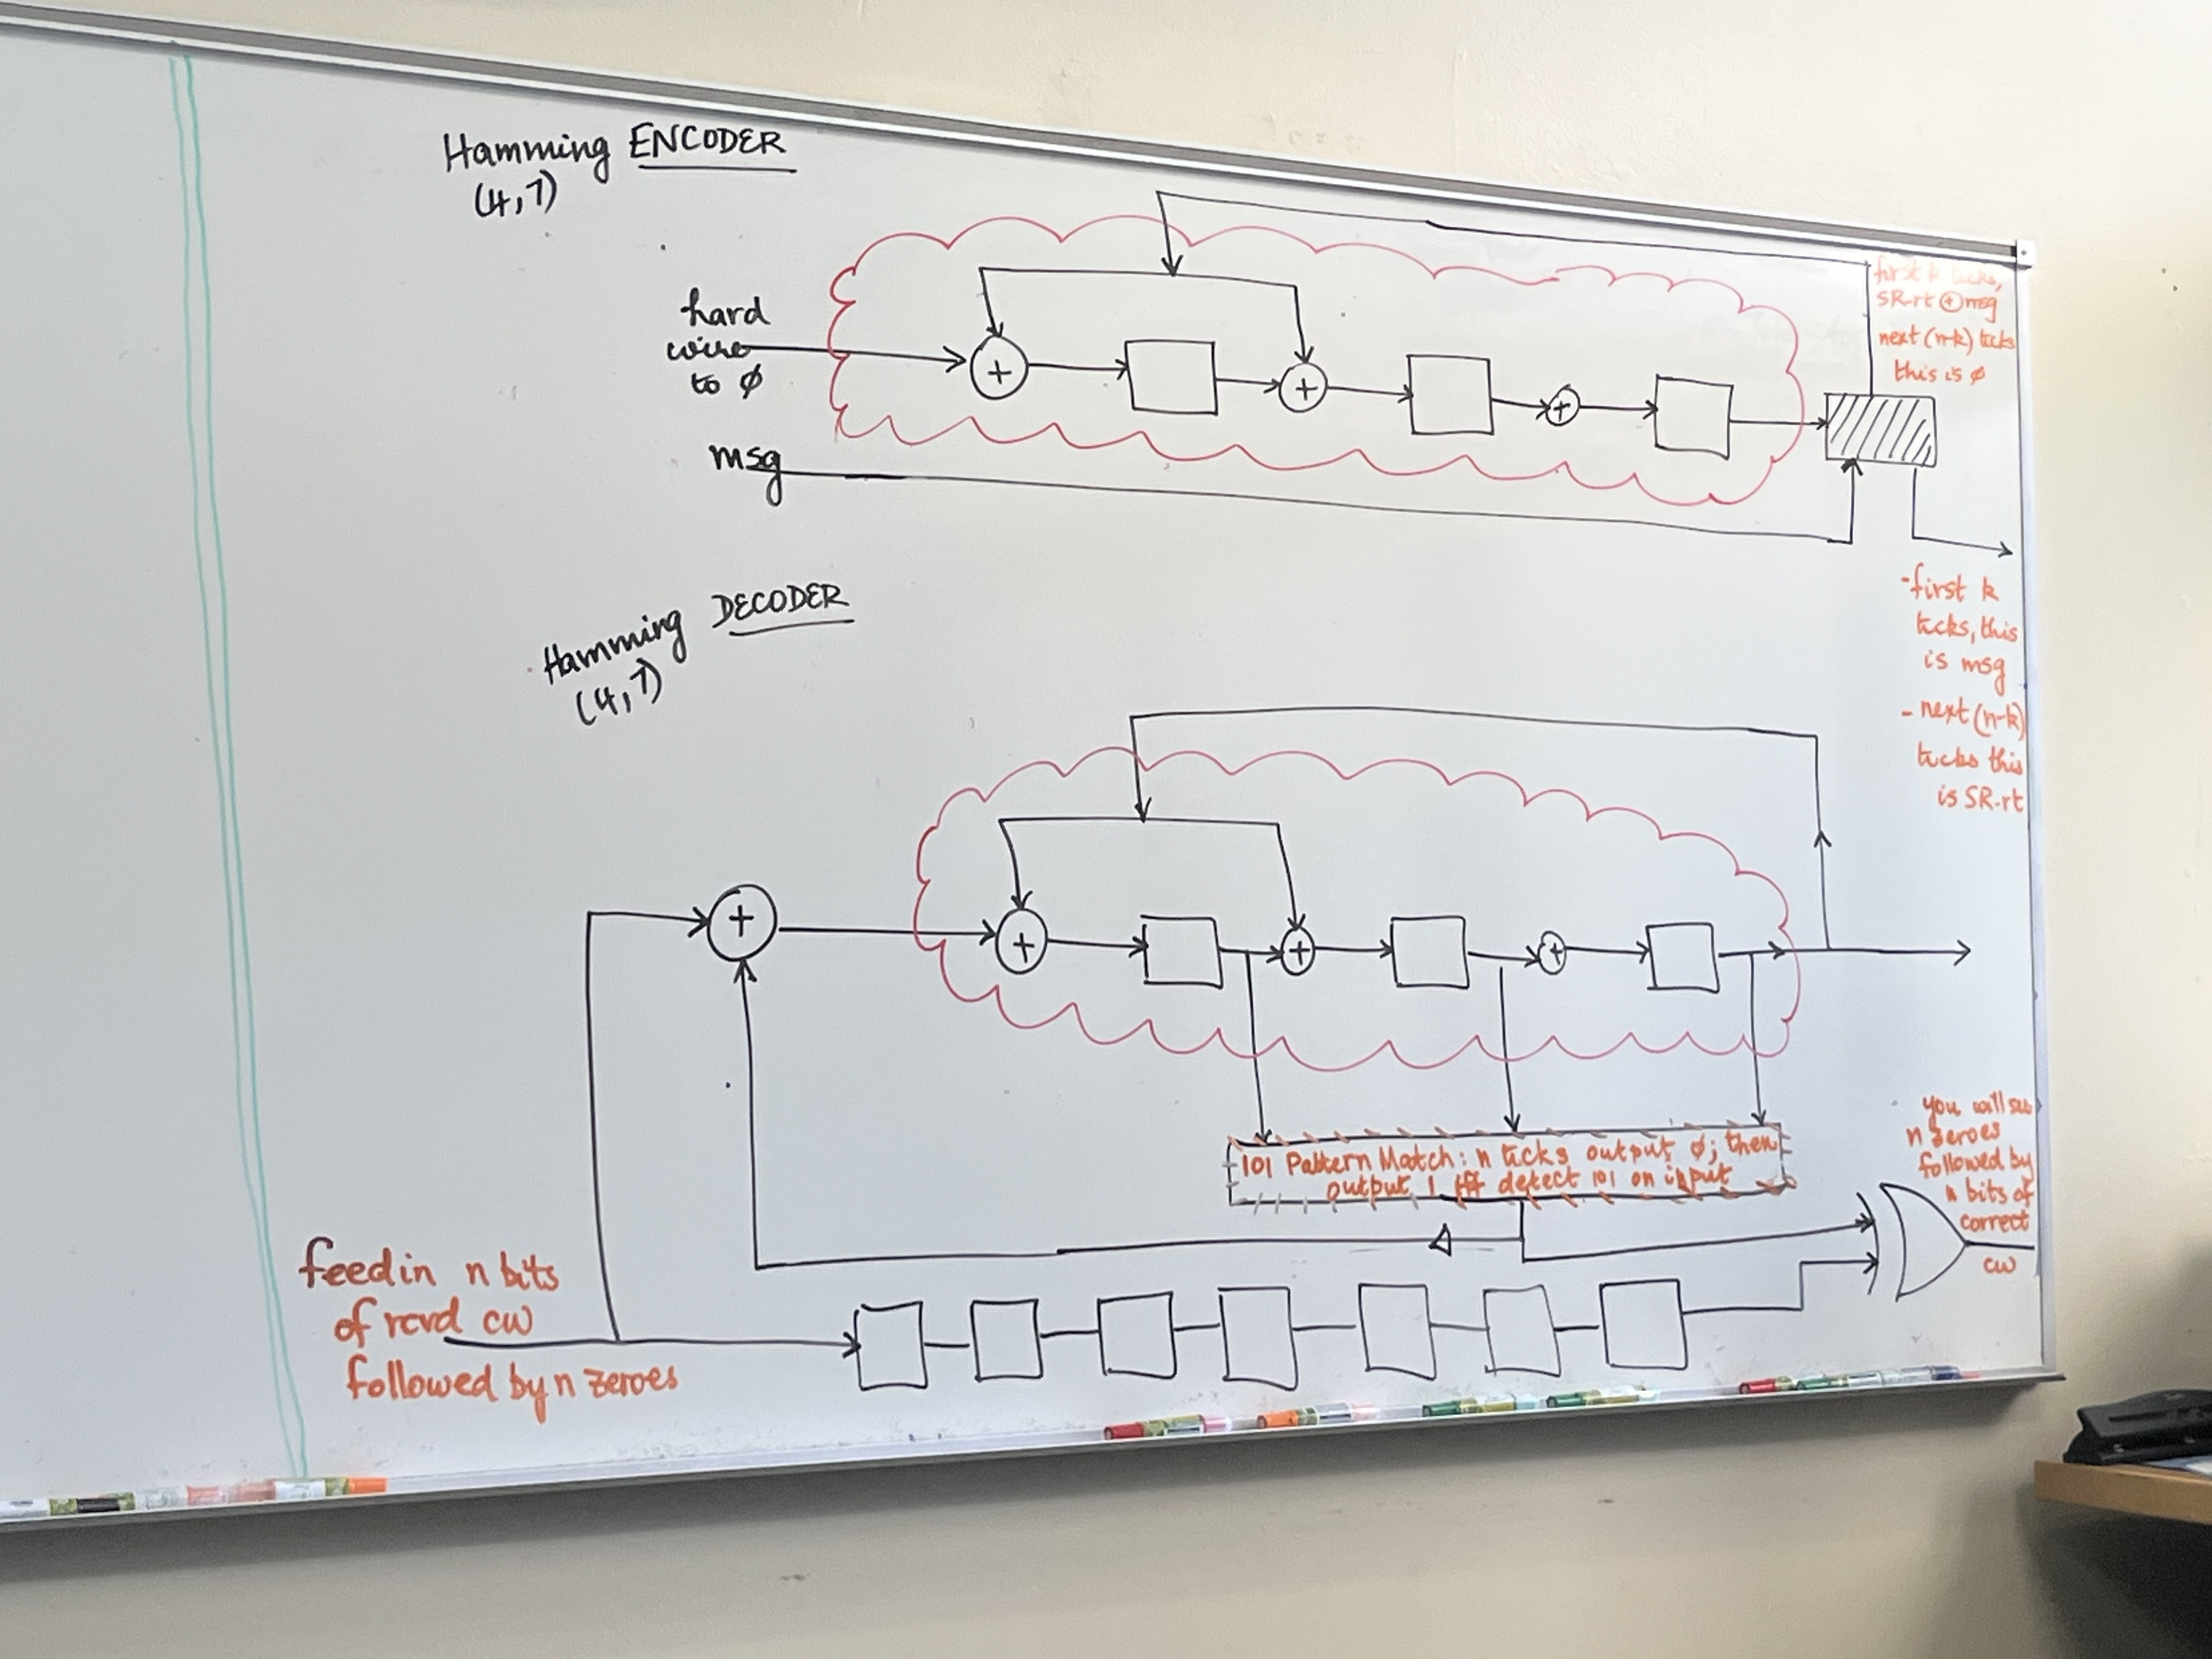
\includegraphics[width=\textwidth]{hammingEncoderDecoder.jpg}

In general, let us feed $c_4c_3c_2c_1$ into the machine from right to left, so that it will read $c_1, c_2, c_3, c_4, 0, 0, 0;$ denote $c_{ij}:=c_i\oplus c_j$ and $c_{ijk}:=c_i\oplus c_j\oplus c_k.$


\begin{tabular}{|c|c|c||c|c|}
    \hline
     Step & SR Out (3 bits) & Message (1 bit) & SR In/Top (1 bit) & Codeword (1 bit)  \\
     \hline
     1& 000&$c_1$& $c_1$&$c_1$\\
     2& $c_1c_10$ & $c_2$&$c_2$&$c_2$\\
     3& $c_2c_{12}c_1$ & $c_{3}$&$c_{13}$&$c_3$\\
     4& $c_{13}c_{123}c_{12}$ & $c_4$&$c_{124}$&$c_4$\\
     5& $c_{124}c_{234}c_{123}$ & 0&0&$c_{123}$\\
     6& $0c_{124}c_{234}$ & 0&0&$c_{234}$\\
     7& $00c_{124}$ & 0&0&$c_{124}$\\
     \hline
\end{tabular}

This is because $c_{11234}=c_{11}\oplus c_{234}=c_{234}.$

Now decoder. Note that there is the same shift register inside the decoder as in the encoder. 


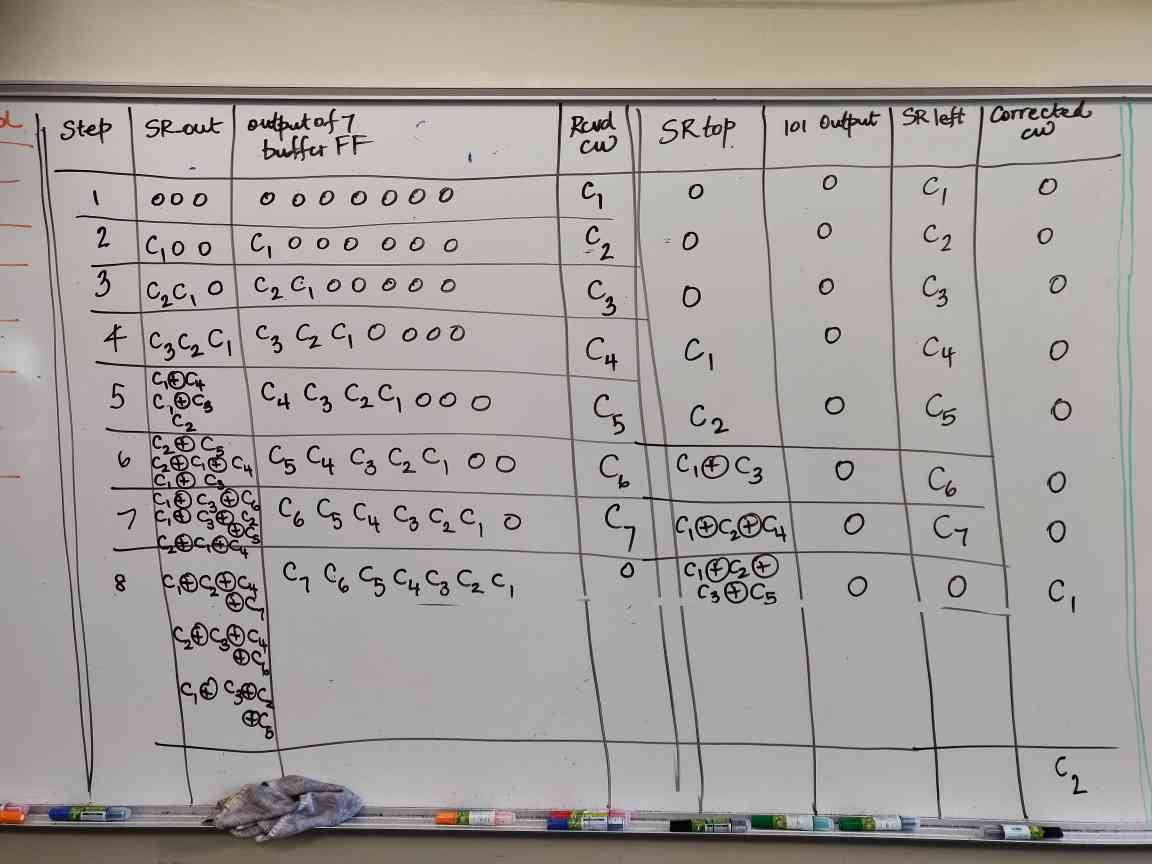
\includegraphics[width=\textwidth]{hammingDecoder.jpg}

\subsection{Hamming Decoder and Generating Functions}
 
Look at the figure in the previous section. Note that on step 8,
\[c_1\oplus c_2\oplus c_3\oplus c_5=0\] since
$c_5=c_1\oplus c_2\oplus c_3$
assuming there are no errors, so these combinations of 4 XORS are double checking the bits $5,6,7.$

Now assume the error is in $c_3.$


\begin{tabular}{|c|c|c||c|c|}
    \hline
     Step & SR Out (3 bits) & Buffer (7 bits) & SR In/Top (1 bit) & Codeword Out (1 bit)  \\
     \hline
     8& $c_{1247}c_{2346}c_{1325}=011$&$c_7c_6c_5c_4c_3c_2c_1$& $c_{1325}=1$&$c_1$\\
     9& $ 111 $ & $0c_7c_6c_5c_4c_3c_2$ & 1 & $c_2$ \\
     10& $101 $ & $00c_7c_6c_5c_4c_3$& 1 &$c_3 \oplus 1$\\
     11& $100$ & $\dots$ & 0 & $c_4$\\
     12& $010$ &  & 0 & $c_{5}$\\
     13& $001$ &  &1&$c_{6}$\\
     14& $110$ &  &0&$c_{7}$\\
     \hline
\end{tabular}
Notice how the SR Out column forms a cycle! This is how the pattern 101 corrects errors by locating its position. If there were no errors, SR Out would have started at $000$ and never moved. This is a Galois linear feedback shift register.

\paragraph{All Kinds of Codes}
Hamming codes are a kind of block code, because they act on a block of 4 bits, mapping it to 7 bits. A special kind of block code is a cyclic code, for which a codeword can be shifted around while still working. Some kinds of cyclic codes are Hamming codes, BCH codes, and Reed Solomon codes, which form a family of codes. Golay codes are a also cyclic, but they stick out from the other codes (Steiner system reference). Why?
Hamming:

\begin{tabular}{c|c|c}
k&n&e\\
\hline
4&7&1\\
11&15&1\\
26&31&1\\
\dots&\dots&\dots
\end{tabular}


BCH:

\begin{tabular}{c|c|c}
k&n&e\\
\hline
7&15&2\\
5&15&3\\
21&31&2\\
17&31&5\\
\dots&\dots&\dots
\end{tabular}

Reed-Solomon codes:
These are special because they correct bytes, not bits.

\begin{tabular}{c|c|c}
k&n&e\\
\hline
$223\times 8$&$255\times8$&$16\times8$\\
\dots&\dots&\dots
\end{tabular}

But, Golay codes only word for one combination of $k,n,e$:

\begin{tabular}{c|c|c}
k&n&e\\
\hline
12&23&3\\
\end{tabular}


Other than block codes, there are also things such as convolutional codes (i.e. Viterbi code). Unlike Block codes, these codes have memory, so a message might not produce the same codeword if run multiple times.

In real life, block codes are normally cyclic because they can be efficiently done with things like shift registers.

Engineers: bits, Mathematician: elements of the field $\mathbb{F}_2=GF(2)=\mathbb{Z}/2\mathbb{Z}.$

A code is identified by a generator polynomial. Hamming codes have a function
\[g(x)=x^3+x+1\] over $\mathbb{F}_2.$



Why does $x^3+x+1$ work based on the shift register design? Consider the taps on 1 and 2. This corresponds to $x^0=1$ and $x^1=x,$ and because it is a Hamming (4,7), we add on a $x^3,$ because $3=n-k=7-4.$

\paragraph{Design of Encoder and Decoder}

There are two different views of the world.


\begin{tabular}{c|c}
Engineer (Shift Register)&Mathematician (Polynomials over $\mathbb{F}_2$)\\
\hline
Bits (0/1)&Elements of $\mathbb{F}_2$\\
XOR of 2 bits & Addition of two elements\\
AND & Multiplication of two elements\\
String of bits (1011001)&$x^6+0x^5+x^4+x^3+0x^2+0x+1.$\\
Bitwise XOR of two strings & Sum of 2 polynomials\\
Convolution of two strings & Product of two polynomials
\end{tabular}

For an example consider 110 $(x^2+x)$ and 11001 $(x^4+x^3+1),$
We have
\[(x^2+x)(x^4+x^3+1)=x^6+x^4+x^2+x.\]

Now convolve these two bits:
\[1100100+110010+00000=1010110\to x^6+x^4+x^2+x\]
Convolution: We reverse one string and slide them past each other. This was also how we added the PDFs of random variables, adding together the probability of all possible pairs that sum to x. In terms of polynomial multiplication, we look at all possible pairs that get a term of degree $x$.
\[
(f \ast g)[x]= \sum_t f[t] g[x-t].
\]

Going back to Hamming $(7,4,1)$ and
\[g(x)=x^3+x+1,\]
let us try to encode it:
If our message polynomial is
$m(x)=c_1x^3+c_2x^2+c_3x+c_4,$
then our output polynomial is
$c(x)=c_1x^6+c_2x^5+\dots+c_7.$
How do we get it?

\begin{enumerate}
\item Find $x^3 m(x)$
\item $r(x)=x^3m(x)\mod g(x),$
\item $c(x)=x^3m(x)-r(x)=x^3m(x)+r(x).$
\end{enumerate}

If our message is $1010,$ then $m(x)=x^3+x.$
$m(x)x^3=x^6+x^4.$

$m(x)x^3\pmod{g(x)}=x+1.$

$c(x)=x^6+x^4-x-1=x^6+x^4+x+1\to 1010011$
\subsection{Encoding and Decoding Math and Channel Coding Theorem}
Recall the encoder:
\begin{enumerate}
\item Find $x^3 m(x)$
\item $r(x)=x^3m(x)\mod g(x),$
\item $c(x)=x^3m(x)-r(x)=x^3m(x)+r(x).$
\end{enumerate}

Decoder: We have some seven bit codeword $c'$ with gf $c'(x)=c_1'x^6+c_2'x^5+\dots+c_7'.$ We want $m'(x)=m'_1x^3+m'_2x^2+m'_3x+m'_4.$
\begin{enumerate}
    \item Let $r'(x)=c'(x)\pmod{g(x)}$
    \item If $r'(x)=0,$ there are no errors, so $m'(x)=m(x),$ which is the $c'(x)$ truncating the last 3 bits, is sent.
    \item If $r'(x)\ne0,$ there must be at least one error. Assuming there is only one (because that is our capability).
    \item Compare $r'(x)$ to the different remainders to find the wrong bit (see below).
\end{enumerate}

Consider the remainders of $x^n$ when divided by $g(x)=x^3+x+1.$
\[x^6\to x^2+1,x^5\to x^2+x+1,x^4\to x^2+x,x^3\to x+1,x^2\to x^2,x\to x,1\to 1.\]
In binary:
\[101,111,110,011,100,010,001.\]
Note 101 is the remainder of $x^6,$ just like in our decoder. If we see any of these remainders, we compare them to the gfs' remainders.

If our code is 
\[c'(x)=c(x)+e(x),\]
then
\[c'(x)\mod{g(x)}=[c(x)+e(x)]\mod{g(x)}=e(x)\mod{g(x)},\]
since $c(x)\equiv 0\mod{g(x)}.$
\paragraph{Example}
Message: 1011, $m(x)=x^3+x+1,$ so $c(x)=x^6+x^4+x^3.$


Codeword: 1100001, $c'(x)=x^6+x^5+1,$ so $r'(x)=x+1\ne 0,$ so there is an error in the $x^3$ term. So, $c'(x)=x^6+x^5+x^3+1,$ so $m(x)=1101.$

Just for fun, Hamming (15,11,1): $g(x)=x^4+x+1.$

Hamming (15,7,2): $g(x)=x^8+x^7+x^6+x^4+1.$

Golay (23,12,3): $g(x)=x^11+x^9+x^7+x^6+x^5+x+1.$


\subsubsection{Channel Coding Theorem}
$H(X)$ is the lower bound of the performance of any source encoder of decoder (this is the Source Coding theorem). Similarly, we will prove that $C(Y|X)$ is an upper bound on the performance of any channel encoder or decoder. 

\begin{figure}
    \centering
    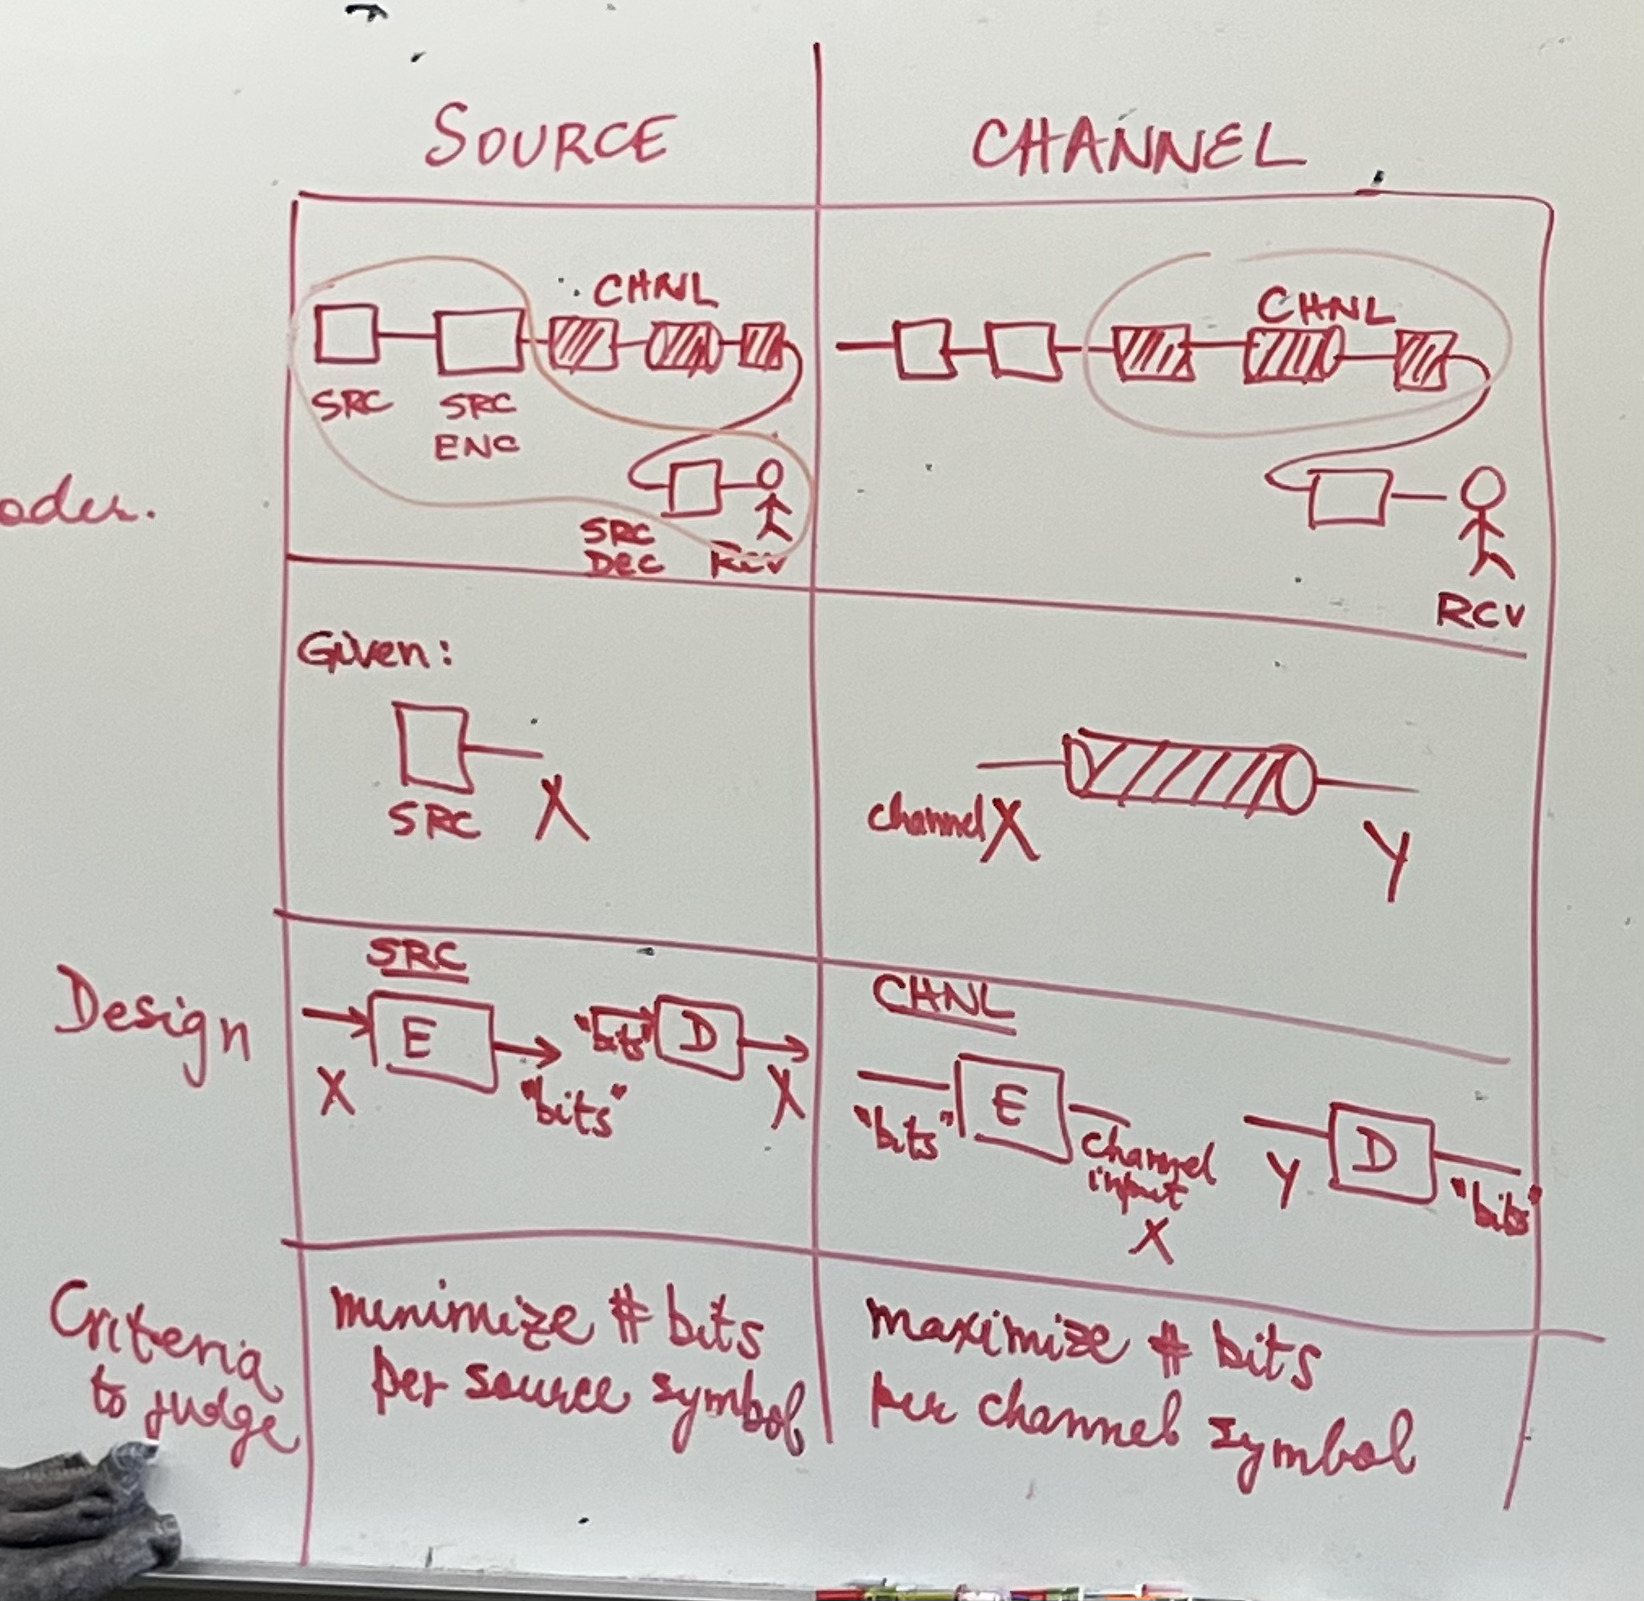
\includegraphics[width=0.7\linewidth]{src_chan.jpeg}
\end{figure}

Lemma 1:
\[I(\langle u_1,u_2,\dots,u_R\rangle;\langle v_1,v_2,\dots,v_R\rangle)\le I(X;Y).\]

Lemma 1.5:
\[R\cdot I(u_i;v_i)\le I(\langle u\rangle;\langle v\rangle)\]
Lemma 2 (Fano):
\[H(u_i|v_i)\le H(P_{err})\]

Combining these, we get
\[R\cdot I(u_i;v_i)\le I(\langle u\rangle;\langle v\rangle)\le I(X;Y)\le C(Y|X).\]
Also, \[I(u_i;v_i)=H(u_i)-H(u_i|v_i)=1-H(u_i|v_i)\ge 1-H(P_{err}).\] For simplicity, just assume that the $u_i$ are fair and independent coin tosses. This yields
\[C(Y|X)\ge R(1-H(P_{err}).\] We have
\[R\le\frac{C(Y|X)}{1-H(P_{err})},\] which is a bound on the number of symbols that can be sent. As $P_{err}\to 0,$ we find that $R\to C(Y|X),$ so the number of symbols is bound by the channel capacity.


\subsection{Channel Coding Theorem (12.02.2024)}
We prove that the channel capacity $C(Y|X)$ is the upper bound of the amount of stuff you can send.

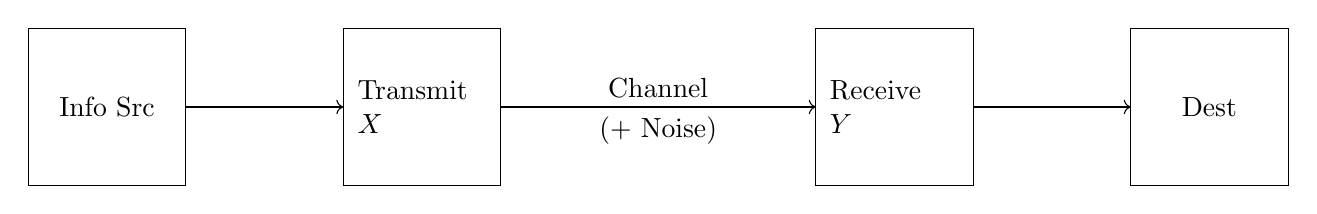
\begin{tikzpicture}[scale=2]
\draw[black] (-4, 0) rectangle (-3, 1) (-2, 0) rectangle (-1, 1) (1, 0) rectangle (2, 1) (3, 0) rectangle (4, 1);
\draw[->] (-3, 0.5) -- (-2, 0.5);
\draw[->] (-1, 0.5) -- (1, 0.5);
\draw[->] (2, 0.5) -- (3, 0.5);
\draw (-3.5, 0.5) node[anchor=center] {Info Src}
    (-1.9, 0.5) node[anchor=center,text width=1] {Transmit \\ $X$}
    (1.1, 0.5) node[anchor=center,text width=1] {Receive \\ $Y$}
    (3.5, 0.5) node[anchor=center] {Dest}
    (0, 0.5) node[anchor=south] {Channel}
    (0, 0.5) node[anchor=north] {(+ Noise)};
\end{tikzpicture}

\[\langle u_1,u_2,u_3,\dots,u_k\rangle\to X\to Y\to\langle v_1,v_2,v_3,\dots,v_k\rangle\]

\paragraph{Lemma 1}
Per block:
\[I(\vec{U};\vec{V})\le I(\vec{X};\vec{Y})\]
or Per Symbol:
\[kI(U;V)\le nI(X;Y)\]

Consider we have a Markov Chain \[A \to B \to C.\]
We want to prove that 
$I(A;C)\le I(B;C),$
i.e.
\[I(A;C)-I(B;C)\le 0.\]

Consider the expected value (This comes from $I(A;C) = H(A|C) - H(C)$, with the $H(C)$ terms cancelling out. You also need to Bayes theorem to reverse the conditional probability and use the definition of conditional entropy.):
\begin{align*}\mathbb{E}_{AC}\left[\log\frac{p(c|a)}{p(c)}\right]-\mathbb{E}_{BC}\left[\log\frac{p(c|b)}{p(c)}\right]&=\mathbb{E}_{ABC}\left[\log\frac{p(c|a)}{p(c)}\right]-\mathbb{E}_{ABC}\left[\log\frac{p(c|b)}{p(c)}\right]\\
&=\mathbb{E}_{ABC}\left[\log\frac{p(c|a)}{p(c|b)}\right]\\
&\le\log\left(\mathbb{E}_{ABC}\left[\frac{p(c|a)}{p(c|b)}\right]\right)\\&=\log 1=0,\end{align*}
by Jensen.
This is because
\begin{align*}\mathbb{E}_{ABC}\left[\frac{p(c|a)}{p(c|b)}\right]&=\sum_{a,b,c}p(a,b,c)\frac{p(c|a)}{p(c|b)}\\
&=\sum_{a,b,c}p(a)p(b|a)p(c|b)\frac{p(c|a)}{p(c|b)}\\&=\sum_{a,b,c}p(a)p(b|a)p(c|a)\\&=\sum_{a,b,c}p(b|a)p(a,c)\\&=\sum_{a,b}p(b|a)p(a)\\&=\sum_{a,b}p(a,b)=1.\end{align*}
By data processing inequality, since $C$ only depends on $B$ and not $A,$ we can expand $p(a,b,c)$ like that. Something something markov property? yeah

By the same logic, $I(A;C)\le I(A;B).$
Why? Going backwards,
\[I(A;C)-I(A;B)\le 0\]
\[\mathbb{E}_{AC}\left[\log\frac{p(a|c)}{p(a)}\right]-\mathbb{E}_{AB}\left[\log\frac{p(a|b)}{p(a)}\right].\]
And continue as before.
Going back to our channel model, we have the markov chain
\[U\to X\to Y\to V,\] so we have
$I(U;V)\le I(U;Y)\le I(X;Y),$ proving Lemma 1.

\paragraph{Lemma 2}
\[H(u_i|v_i)\le H(P_{err}).\]
We are dealing with a \textbf{binary channel}. If there is an error, there is only one possibility and can be corrected by flipping the bit.
We define $P_{err}$ to be the probability that the bit sent into the encoder is received wrongly out of the decoder, so $v_i\ne u_i$ is received.

If you know the bits to $X$ translation in the encoder and $p(y|x)$ of noise in the channel and the $Y$ to bits translation of the decoder, we can determine $P_{err}$ exactly.

Toss a coin with weight $P_{err},$ if heads then you know that you have to flip it, but if tails then you know that it is right with no uncertainty, so
\[H(u_i|v_i)\le H(P_{err}).\]
(it is actually equal but no one cares)

From Lemma 1,
\[\frac{k}{n}I(u_i;v_i)\le I(X;Y)\le C(Y|X).\]
From Lemma 2,
\[I(u_i;v_i)=H(u_i)-H(u_i|v_i)\ge 1-H(P_{err}),\]
assuming that $u_i$ is $0$ or $1$ uniformly (on average), which is the worst we can send. Again this is also an equality but dw about it.
Combining them,
\[\frac{k}{n}\le \frac{C(Y|X)}{1-H(P_{err})}.\] Letting $P_{err}\to 0,$ we see that
\[\frac{k}{n}\le C(Y|X).\]
We can consider $k/n$ to be the rate of data through the channel. Recall that for source coding, we knew of a way to almost get to the lower entropy bound (Huffman is within one), but for channel coding there isn't a way to get to the upper bound.

\paragraph{Geometric Intuition of Codes}
We need a hypercube graph. If a 1d hypercube graph is a single vertex, we define an $n$d hypercube graph to be two copies of an $n-1$d hypercube graph with the corresponding edges connected. 
\begin{figure}[bt]
 \centering
 \scalebox{0.6}
 {
 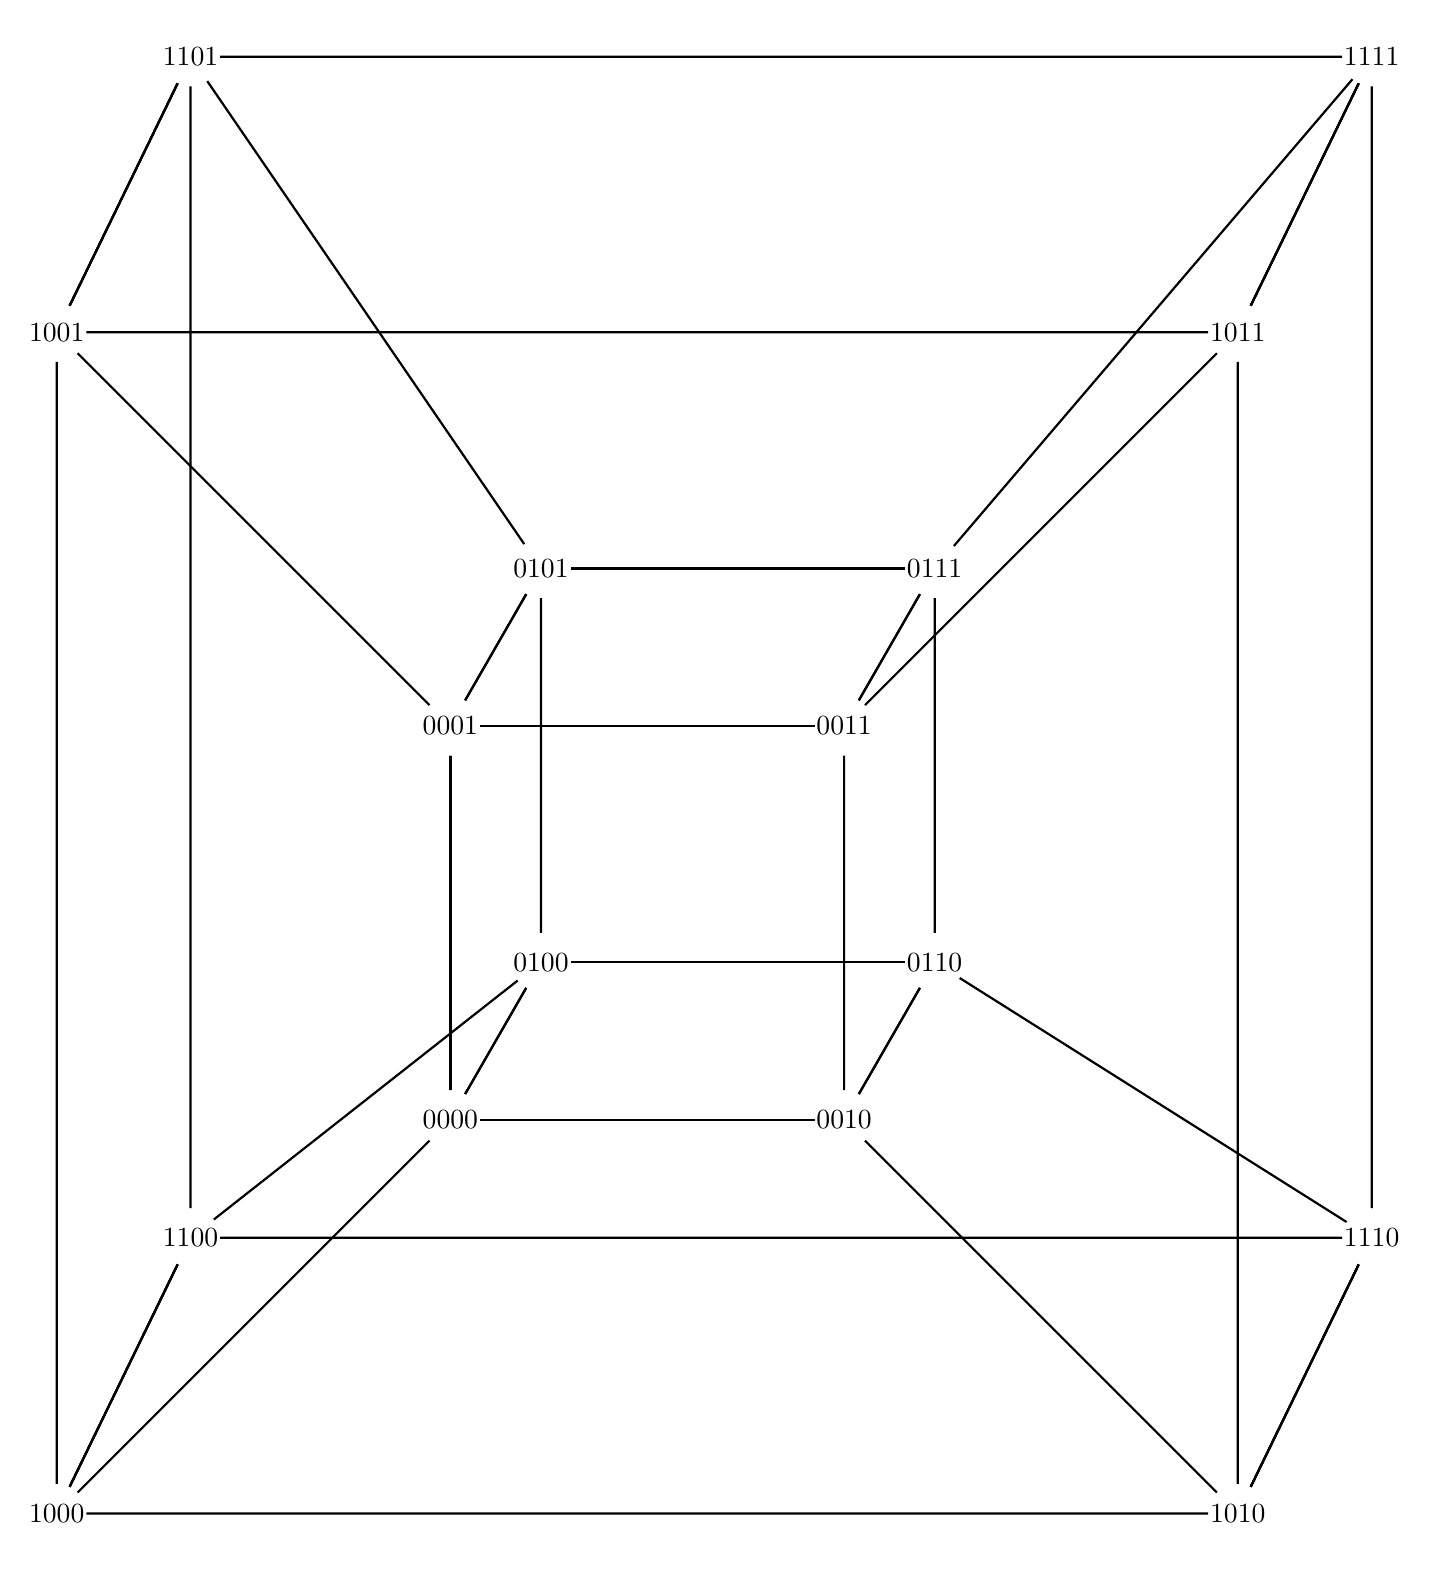
\begin{tikzpicture}[scale=5]
	 \tikzstyle{vertex}=[circle,minimum size=20pt,inner sep=0pt]
	 \tikzstyle{edge} = [draw,thick,-,black]
	 \node[vertex] (v0) at (0,0) {$0000$};
	 \node[vertex] (v1) at (0,1) {$0001$};
	 \node[vertex] (v2) at (1,0) {$0010$};
	 \node[vertex] (v3) at (1,1) {$0011$};
	 \node[vertex] (v4) at (0.23, 0.4) {$0100$};
	 \node[vertex] (v5) at (0.23,1.4) {$0101$};
	 \node[vertex] (v6) at (1.23,0.4) {$0110$};
	 \node[vertex] (v7) at (1.23,1.4) {$0111$};
	 \node[vertex] (v8) at (-1,-1) {$1000$};
	 \node[vertex] (v9) at (-1,2) {$1001$};
	 \node[vertex] (v13) at (-0.66,2.7) {$1101$};
	 \node[vertex] (v12) at (-0.66,-0.3) {$1100$};
	 \node[vertex] (v10) at (2,-1) {$1010$};
	 \node[vertex] (v14) at (2.34,-0.3) {$1110$};
	 \node[vertex] (v11) at (2,2) {$1011$};
	 \node[vertex] (v15) at (2.34,2.7) {$1111$};
	 \draw[edge] (v0) -- (v1) -- (v3) -- (v2) -- (v0);
	 \draw[edge] (v0) -- (v4) -- (v5) -- (v1) -- (v0);
	 \draw[edge] (v2) -- (v6) -- (v7) -- (v3) -- (v2);
	 \draw[edge] (v4) -- (v6) -- (v7) -- (v5) -- (v4);
	 \draw[edge] (v8) -- (v9) -- (v13) -- (v12) -- (v8);
	 \draw[edge] (v0) -- (v4) -- (v12) -- (v8) -- (v0);
	 \draw[edge] (v1) -- (v9) -- (v13) -- (v5) -- (v1);
	 \draw[edge] (v2) -- (v10) -- (v14) -- (v6) -- (v2);
	 \draw[edge] (v8) -- (v10) -- (v14) -- (v12) -- (v8);
	 \draw[edge] (v3) -- (v11) -- (v15) -- (v7) -- (v3);
	 \draw[edge] (v10) -- (v11) -- (v15) -- (v14) -- (v10);
	 \draw[edge] (v9) -- (v11) -- (v15) -- (v13) -- (v9);
 \end{tikzpicture}
 }
 \end{figure}
We can also think of the $n$d hypercube graph as $2^n$ vertices labeled in binary from $00\dots0$ to $11\dots 1,$ where two vertices are connected by an edge if they differ by exactly one bit. This will yield
$n\cdot 2^{n-1}$ edges. We define the distance $d(x,x')$ between two vertices $x$ and $x'$ to be the minimum number edges between them, or, alternatively, the number of positions that $x$ and $x'$ differ bitwise. This is known as the Hamming distance.

\subsection{Hamming ``Sphere'' or Something (12.04.2024)}
We define the Hamming ``sphere'' at node $x$ with radius $r$ is the set of all nodes on the Hamming hypercube that are $\le r$ units away from $x.$ 
\[\text{``Sphere''}(x,r):=\{x'|d(x,x')\le r\}.\]
We find that the volume of the ``sphere'' is
\[\sum_{k=0}^{\lfloor r\rfloor}\binom{n}{k}.\] This is because there are $\binom{n}{k}$ ways to pick $k$ bits to flip out of an $n$-bit number. Now, we can determine if a code is good. 

Consider a source coder that maps $2^k\to 2^m.$  

Recall how a cyclic code works: If there are $2^k$ red nodes in the $2^n$ space (valid codewords), such as $\langle b_1,b_2,\dots,b_n\rangle,$ then $\langle b_n,b_1,\dots,b_{n-1}\rangle$ is also a red node. (idk why we are talking about these)

If a blue dot comes out of the channel, we snap to the closest red dot, which would hopefully fix the error. Naturally, we ask how many errors can be corrected.
\begin{enumerate}
    \item For every red dot, blow a balloon from radius zero
    \item Grow the balloons simultaneously
    \item Stop when two touch
    \item Take a step back, where the radius is $R.$
\end{enumerate}
$R$ is the maximum number of errors you can correct. If there are more than $R$ errors, you cannot guarantee an accurate decoding.

Let $c_i$ and $c_j$ be some red codewords. Then
\[d_{min}=min_{i\ne j}d(c_i,c_j),\]
and 
\[R=\left\lfloor\frac{d_{min}-1}{2}\right\rfloor=\left\lfloor\frac{d_{min}}{2}\right\rfloor-1.\]

Imagine a $(4,10)$ code. Since the volume of a sphere of radius $3$ in a 10-d hypercube is 
\[\binom{10}{0}+\binom{10}{1}+\binom{10}{2}+\binom{10}{3}=176,\]
and there are $2^4$ red codes, so there would have to be
$176\cdot 2^4$ nodes, which is greater than $2^{10},$ so it is impossible.
\paragraph{WHAT IS ON THE TEST}
\begin{enumerate}
    \item Channel capacity (Mutual information, KL Divergence ($D(p||q)$), Binary Symmetric Channel, Binary Erasure Channel)
    \item Channel Codes (Shift Registers, Generating Polynomials, Hypercube Geometry intuition)
    \item Channel Coding Theorem
\end{enumerate}
\subsection{Guest Speaker Professor Beth Malmskog (12.06.2024)}
\paragraph{Introduction to Error Correcting Codes}
She studies locally-recoverable codes using algebraic geometry and number theory, as well as code-based post-quantum cryptography based off error correcting codes.

A code is any system for communicating information, and the alphabet is the set of symbols (actions, words, morse code etc.) used in the system. Communication consists of not only communicating across distance but also across time (storage). For example, books do this, as well as something like floppy disks.

Digital codes: Every symbol is translated into a string (vector) of digits. Every meaningful vector in a system is called a codeword. For example, for an image, we can encode each pixel as a number into a longer vector. The set of all codewords is a code.

We also need to build redundancy into our codes, not only because of human error but also due to electronic and mechanical errors. For example, error detecting codes can be used to determine if an error happened. Consider $\mathbb{Z}/n\mathbb{Z},$ the integers modulo $n$ under addition, where two numbers $a$ and $b$ are considered equivalent if they have the same remainder when divided by $n.$ You can think of this as counting on a clock. Consider the ``Mod Detecting Code,'' other wise known as a Universal Product Code (UPC), which consists of 11 digits of product information (like the label of an item or any other info) and a 12th check digit. If the first 11 digits are $d_1,d_2,\dots,d_{11},$ then we define the 12th digit $d_{12}$ to be the digit such that
\[3d_1+d_2+3d_3+d_4+\dots+3d_{11}+d_{12}\equiv 0\pmod{10}.\]

If the first 11 digits are 09661911248, then the 12th digit would be 7. But why are we multiplying every other digit by 3? This is because we can detect some wrongful digit swaps. Ok, how do we correct errors? Send the message three times and do majority rules for each bit. But this isn't very efficient.

\paragraph{Hamming Codes}To be more efficient, we can use Hamming codes. We know how this works, go back up in the notes if you want to review them. Hamming codes have 16 legal codewords.

What makes a good code?
First, we want efficiency. A code has length $n$ if each codeword is a vector of $n$ symbols. There are $k$ information symbols if it takes $k$ symbols to send.

We also want effectiveness, that is to correct many errors. We define the Hamming distance of two vectors to be the number of digit places where they are different. The minimum distance of a code is the smallest distance between two distinct codewords of a code. If we find a $\vec{w}$ such that
\[d(\vec{v},\vec{w})\le \frac{d-1}{2},\] we know that it is probably meant to be $\vec{v}.$ if there are up to $d-1$ errors, we will correct wrongly but detect a code regardless.

Theorem: Singleton Bound. If a code has a length $n,$ a minimum distance $d$ and if each codeword has $k$ information symbols, then
\[d\le n-k+1,\] and if equality happens, then the code is called a maximum distance separated (MDS) code. Hamming codes are not an MDS code, since 
\[7-4+1=4,\] but $d=3$ so it isn't perfect.

\paragraph{Reed-Solomon codes}
Let $q$ be prime, and let $\vec{a}=(0,1,2,\dots,q-1)$ be the elements of $\mathbb{Z}/q\mathbb{Z}.$ (This actually works for the integers mod $q^n$ in general). Let $1\le k\le q.$ This is the dimension of the code. Define $L_{k-1}$ to be the set of polynomials $g(x)$ of $\mathbb{Z}/q\mathbb{Z}[x]$ with degree $\le k-1.$ For every $g\in L_{k-1},$ we define $g(\vec{\alpha})=(g(0),g(1),\dots,g(q-1)),$ evaluating the polynomials in $\mathbb{Z}/q\mathbb{Z}.$ The Reed-Solomon code is defined as
\[RS(k,q)=\{g(\vec{\alpha}):g\in L_{k-1}\}.\] Every polynomial of degree at most $k-1$ gives a vector of length $q$ in $RS(k,q).$

Example:
Let $q=5$ and $k=3.$ If $g(x)=x^2-4x+3=x^2+x+3,$ then we have $g(\vec\alpha)=(3,0,4,0,3).$ The function has three degrees of freedom (information symbols) and the length of the code is 5, and there are $5^3$ total codes. Note that every polynomial in $L_2$ is a linear combination of $\{1,x,x^2\}$ over $\mathbb{F}_5,$ since
\[g(x)=a+bx+cx^2\]
with $a,b,c\in\mathbb{Z}/5\mathbb{Z}.$ If $f_1(x)=1,f_2(x)=x,f_3(x)=x^2,$
then
\[f_1(\vec{\alpha})=(1,1,1,1,1), \quad f_2(\vec{\alpha})=(0,1,2,3,4), \quad f_3(\vec{\alpha})=(0,1,4,4,1),\] and this forms a basis of the $RS(3,5)$ code. Is it a good code? Every quadratic polynomial is determined by 3 coefficients, so there are three information symbols. If we have two distinct quadratic polynoimals, they can intersect in $0,1,$ or $2$ points. Similarly, $\mod$ q, they can intersect in 2 points, so the minimum distance at least $5-2=3.$ The Singleton bound yields $d\le n-k+1=3,$ so RS is optimal! We don't want $k$ to be too big, for example if $k=q$ then there is no minimum distance which is bad. Depending on $k,$ we can do the trade-off between $k$ and distance. The way that we can determine the polynomial given the codeword is the polynomial interpolation algorithm. Reed-Solomon codes are still really popular in things like music storage.

Since there are $q^k,$ and we need a lot of codewords, we need a large prime $q,$ which isn't very efficient for calculating on computers. Instead of using the values of $\mathbb{Z}/q\mathbb{Z},$ which can be thought of as points on a line, we can consider points on a curve $\mathcal{X},$ which is the solution to some high dimensional multivariable polynomial. This lets you do coding faster.

\paragraph{Cloud Storage}
What kind of errors occur in cloud storage? The idea in cloud storage is spreading a codeword across many servers, so that if one server fails, it can be recovered by thinking of the erasure as just an error, which we know how to fix with error correction. But, we don't like storing each symbol in a different symbol. We want a locally recoverable code, which has the property that each symbol can be recovered by accessing only $r$ different symbols; then $r$ is the locality of the code. The set of symbols used to recover that symbol is called the recovery set of that symbol.

\url{https://en.wikipedia.org/wiki/Berlekamp%E2%80%93Welch_algorithm}.
\url{https://en.wikipedia.org/wiki/Guruswami%E2%80%93Sudan_list_decoding_algorithm}.

The big idea is polynomial interpolation. Remember that if $f(x)$ is a univariable polynomial of degre $m,$ then it is fully determined by $m+1$ points (Lagrange Interpolation). We can use this fact to locally recover an $RS(k,q)$ code. If we erase one symbol, it's like erasing the value of a polynomial in one input. Then, we only have to use $k$ other bits to recover the entire polynomial and the erased bit. But the locality is $k$ which is too big. We can generalize RS codes to a higher dimension. This is the Reed-Muller code.

Let $m$ be a natural number and $q$ prime, then we let $\vec{\alpha}=(\alpha_{1},\alpha_2,\dots,\alpha_{q^m}),$ where $\alpha$ is a point in $m$ dimensional space $(\mathbb{Z}/q\mathbb{Z})^m.$ If $1\le v\le q-2,$ we can let $M_v$ be the set of polynomials $g(x_1,x_2,\dots,x_m)$ with coefficients in $\mathbb{Z}/q\mathbb{Z}$ and total degree at most $v.$ We let $g(\vec{\alpha})=g(\vec{\alpha_1},\dots,g(\vec{\alpha_{q^m}})).$
We call the Reed-Muller code $RM_q(v,m)=\{g(\vec{\alpha}):g\in M_v.$
Consider $RM_3(2,2),$ which has code length 9.
If $\vec{\alpha}=((0,0),(0,1),\dots,(2,1),(2,2))$ and $g(x,y)=x+y,$ then $g(\vec{\alpha})=(0,1,2,1,2,0,2,0,1).$
For $RM_5(3,2)$ functions are in 2 variables of total degree at most 3 over $\mathbb{Z}/5\mathbb{Z}.$ We can restrict the function to a line, which makes it a function of one variable. Since the total degree is 3, the polynomial over the line must also be of degree 3, so we can recover it with only 4 points. But, there are 5 points on every line, so we have achieved locality. We only have to look at 4 other points to figure out one erased symbol. Since each position has 6 lines through it, we have so many different recover sets (called availability). Unfortunately, the rate is at most $\frac{q-1}{q^2}\to 0,$ which isn't that good. Decoding is also difficult, because it is NP-hard, but that's good because it can be used as cryptography. (\url{https://en.wikipedia.org/wiki/McEliece_cryptosystem})

\section{Putting it All Together}
\subsection{Shannon's Theorem (12.12.24)}
\begin{tabular}{|  c|c|c|}\hline
&Theoretical Bound&Practical Bound\\
\hline
Source&\makecell{$\forall$ source encoder/decoders, \\ the \# of bits per source symbol is  $\ge H(X)$}&\makecell{$\exists$ a source encoder/decoder such that \\ the number of bits per source symbol \\ is around $H(X)$ (e.g. Huffman)}\\ \hline
Channel&\makecell{$\forall$ channel encoders/decoders, \\ the \# of bits/channel symbol is $\le C(Y|X)$}&\makecell{\shrug\  Maybe we can get something \\ that comes close to $C(Y|X)$}\\ \hline
\end{tabular}

\paragraph{Shannon's Theorem}
Given a source $p(x)$ and a channel $p(y|x),$ we are asked to design an encoder and decoder, such that you achieve reliable communication (i.e. $P_{err}\to 0$). Is this possible? YES but... iff $H(X)\ge C(Y|X).$ This is Shannon's theorem.


\newpage
Unuseful Equations:
\[\sum_{n\le x}\mu(n)=O\left(x^{1/2+\epsilon}\right),\]
where 
\[\mu\ast\mathds{1} = I,\] assuming the Riemann Hypothesis.
\[\int_{\partial\Omega}\omega = \int_{\Omega}\mathrm{d}\omega\]
\[\left(u \cdot v\right) \mathbbm{1} = u \wedge \ast v\]
\[\left(\Box+\frac{m^2c^2}{\hbar^2}\right)\psi = 0\]
\[e^{a \frac{\mathrm{d}}{\mathrm{d}x}} f(x) = f(x - a)\]
\[\left(1 - \int \right)^{-1} 0 = e^x\]
\[
e^{-a x} \left(\fdiffn{}{x} - a\right)^k y = \left(\fdiffn{}{x}\right)^k (e^{-a x} y) = 0 \qquad \therefore y = \left(\sum_{n=0}^{k-1} a_n t^n\right) e^{a x}
\]

\end{document}